%essentials packages
\documentclass[a4paper,12pt]{report}
\usepackage{amsmath, amssymb, amsthm}
\usepackage[top=2cm,bottom=2cm,left=2cm,right=2cm]{geometry}
\usepackage{graphicx,color}
\usepackage[backend=bibtex, sorting=none]{biblatex}
\addbibresource{MyReferences}
% optional package
\usepackage[T1]{fontenc}
\usepackage{url}
\usepackage{adjustbox}
\usepackage{float}
\usepackage{}
% table
\usepackage{xcolor}
\usepackage{colortbl}  
\usepackage{array} 
\usepackage{subcaption}
\DeclareGraphicsRule{*}{mps}{*}{}
%\usepackage{rotating}
\usepackage{feynmp}
\usepackage{tikz}
\usepackage{tikz-feynman}
\tikzfeynmanset{compat=1.1.0}
\usepackage{caption}
\usepackage{subcaption}

\parindent 0pt
\parskip 1ex
\renewcommand{\baselinestretch}{1}
\numberwithin{equation}{section}
\renewcommand{\bibname}{References}
\renewcommand{\contentsname}{Contents}
\pagenumbering{roman}

\usepackage{fancyhdr}
\pagestyle{fancy}
\rhead{}
\lhead{\nouppercase{\textsc{\leftmark}}}
\renewcommand{\headrulewidth}{0pt}
\makeatletter
\renewcommand{\chaptermark}[1]{\markboth{\textsc{\@chapapp}\ \thechapter:\ #1}{}}
\makeatother

% Customising chapter headings - sectsty.pdf
\usepackage{sectsty}
\chapterfont{\Large\sc\centering}
\chaptertitlefont{\centering}
\subsubsectionfont{}

% Hyperreferencing and citations
\usepackage{hyperref}
\hypersetup{
    colorlinks,
    citecolor=blue,
    filecolor=blue,
    linkcolor=blue,
    urlcolor=blue
}

% Section symbol
\setcounter{secnumdepth}{3}
\setcounter{tocdepth}{3}
\usepackage{cleveref}
\crefname{section}{\S}{\S\S}
\Crefname{section}{\S}{\S\S}
\crefname{subsection}{\S}{\S\S}
\Crefname{subsection}{\S}{\S\S}

\begin{document}

\newpage
%\pdfbookmark[0]{Main title}{maintitle}
\begin{titlepage}
\begin{center}
\vspace {0.5cm}
\huge{\textbf{Theoretically Predicted Production Cross Section of Single Vector Boson}}\\
\begin{figure}[ht!]
\centering

\includegraphics[scale=0.8]{QAU.jpg}
\end{figure}
\vspace{0.8cm}
\Large{By}\\[0.5cm]
\Large{\textbf{Junaid Tariq}}\\[2cm]
\Large{SUBMITTED IN PARTIAL FULFILLMENT OF THE}\\
\Large{REQUIREMENT FOR THR DEGREE OF}\\
\Large{MASTER OF PHILOSOPHY}\\
\Large{AT}\\
\Large{DEPARTMENT OF PHYSICS}\\
\Large{QUAID-I-AZAM UNIVERSITY,ISLAMABAD}
\end{center}

\end{titlepage}

\newpage
    \pdfbookmark[0]{Certificate}{certificate}
    \chapter*{Certificate} % (fold)
    \label{cha:certificate}
    The undersigned hereby certify that they have read and recommend to the department of physics for acceptance of thesis entitled \textbf{"Theoretically predicted production cross section of Single Vector Boson"} by \textbf{Junaid Tariq} in partial fullfillment of the requirements for the degree of \textbf{Master of Philosophy}.

   
    
 \vspace{3cm}
    \begin{flushleft}
        \line(1,0){100} \\
        Supervisor: \\[0cm]
        Dr. Shamona Fawad Qazi\\
        Associate Professor \\
        Department of Physics\\
        Quaid-i-Azam University\\
        Islamabad.
    \end{flushleft} 
    
    \vspace{3cm}


    \begin{flushleft}
    
   
        \line(1,0){100} \\
        Submitted Through: \\[0cm]
        Dr. Nawazish Ali Khan\\
        Professor\\
        Department of Physics\\
        Quaid-i-Azam University\\
        Islamabad.        
    \end{flushleft}
    


    \newpage
    \pdfbookmark[0]{Copyright Notice}{copyright}
    \chapter*{Copyright Notice} % (fold)
    \label{cha:copyright_notice}
    \begin{flushright}
    \date{}
    \end{flushright}
    \begin{flushleft}
    Author:\hspace{2cm}   \textbf{Junaid Tariq}\\
    Title:\hspace{2cm}    \textbf{"Theoretically Predicted Production Cross Section of Single Vector Boson"}\\
    Department:\hspace{2cm} \textbf{Physics}\\
    Degree:\hspace{2cm} M.Phil\hspace{2cm}Convocation:\hspace{2cm}year:\\[2cm]
    
    Permission is herewith granted to \textbf{Quaid-i-Azam University} to circulate and to have copied for non-commercial purposes, at its discretion, the above title upon the request of individuals or institutions.\\[4cm]
    
  \end{flushleft}
     
     \begin{flushright}
     \line(1,0){150} \\
     Signature of Author
    \end{flushright}        
    % chapter copyright_notice (end)

    % Dedication
    
    \newpage
    \vspace*{8cm}
    \pdfbookmark[0]{Dedication}{dedication}
    \begin{center}
        \Large This thesis is dedicated to \emph{my beloved son}
    \end{center}

   

    % Acknowledgments
    \newpage
    \pdfbookmark[0]{Acknowledgments}{acknowledgments}
    \chapter*{Acknowledgments}
    I cannot express enough thanks to Dr. Nawazish Ali Khan chairman department of physics, for giving me the opportunity to do research in National Center of Physics and providing invaluable guidance throughout this research.\\
        I would like to express my sincere thanks to Dr. Shamona Fawad Qazi for her assistance through my whole duration of M.Phil. She helped me to put my ideas, well above the level of simplicity and into something concrete. I would like to acknowledge his assistance in reading and correcting this thesis.\\  
    I would like to express my special thanks of gratitude to Dr.Wajid Ali Khan who give me the golden opportunity to do this work and also for his patience, kindness and wisdom he has given to me during the whole work. Dr. Wajid Ali Khan is the person who open my mind for the experimental high energy physics. His kind suggestions and words guided me through my whole analysis.\\
   Thanks to all the members in High Energy Physics group at the National
Center for Physics (NCP), especially Dr. Usman Ashraf, Muhammad Gul for their positive criticism and continuous support and encouragement through the early stages of chaos and confusion. Thanks to Dr. Ashfaq Ahmad, Dr. Irfan Ashgar, Dr. Mohammad Ahmed, Sharjeel Kashif, Sheikh Mansoor who helped me in completing this work.\\
The greatest thanks goes to my beloved parents who encouraged me when ever I faced difficulties. Finally, I am grateful to my wife and son. They are always the source of my happiness and encourage me when I am depressed. \\[2cm]

\begin{flushright}
Junaid Tariq\\
November 2021.
\end{flushright}



    % Abstract
    \newpage
    \pdfbookmark[0]{Abstract}{abstract}
    \chapter*{Abstract}
    The cross sections of $Z$ and $W$ boson and their ratios are experimentally measured at the ATLAS and CMS detector at the Large Hadron Collider~(LHC) in proton-proton collision at various center of mass energies. Theoretically predicted cross section of the $W$ and $Z$ boson production cross section in a proton-proton collision at $\sqrt{s}=13~TeV$ and $14~TeV$ are presented in this thesis.

The vector boson production cross section measurement at hadron collision provides a deep understanding of quantum chromodynamics (QCD) and electroweak (EW) processes. The production of $W$ and $Z$ bosons are best examples of hard scattering processes at Large Hadron Collider. Theoretical predictions in perturbative chromodynamics are available at next-to-next-to-leading order~(NNLO).

Theoretically predicted production cross section and cross section ratios of $W$ and $Z$ vector bosons are compared with the measured results at various center of mass energies. Kinematics of these vector bosons and corresponding leptons are also presented.        


    \newpage
    \pdfbookmark[0]{Contents}{contents}
    \tableofcontents

    \listoffigures
    \listoftables

    

    \newpage
    \pagenumbering{arabic}



\chapter{Introduction}
\section{The Standard Model of Particle Physics}
Particle physics deals with the fundamental matter particles and the interactions between them. It also explains their properties such as mass, spin and charge. 
\subsection{The Fundamental Particles}
In particle physics an elementary particle or fundamental particle is the one that has no internal structure or is not made of other particles. The current fundamental particles are called fermions which are called matter particles and other type are called anti-matter particles and bosons, which are the force carrying particles and allow interactions between matter particles.
\subsubsection{Fermions}
In Standard Model~(SM) there are two types of fermions, the quarks and the leptons. The fermions obey the Pauli Exclusion Principle which states that two fermions can not have same state at the same time~i.e.~two fermions can not have same quantum numbers. All fermions have half integral spin. In SM there are twelve fermions which are divided into six generations, each one  has two particles. Fermions are divided into two groups,~leptons and quarks. The leptons have elementary charge of $-1$. Leptons have three flavors of charged particle, electron~$e$, muon~$\mu$ and tau~$\tau$, each lepton has corresponding neutral particle called neutrino. Electron is the only lepton which is stable in the universe from these six leptons. All the other leptons are massive and not stable hence decay into other stable particles.

Quarks have three generations and each one has two types. These six quarks are up~(u), down~(d), strange~(s), charm~(c), bottom~(b) and top~(t). The up~(u) and down~(d) quarks are only stable. The other quarks are very unstable and decay very quickly. Quarks interact with each other by the exchange of particles called gluon. Quarks are the particles which make hadrons~(baryons and mesons).
These twelve fermions have corresponding anti particles called anti-fermions. Electron's antiparticle is positron having same mass but opposite charge of +1, and muon's anti particle is anti muon with charge +1, similarly is the case for all other fermions. Anti-fermion has same mass as that of the corresponding fermion but opposite charge. 

\begin{figure}[h]
\centering
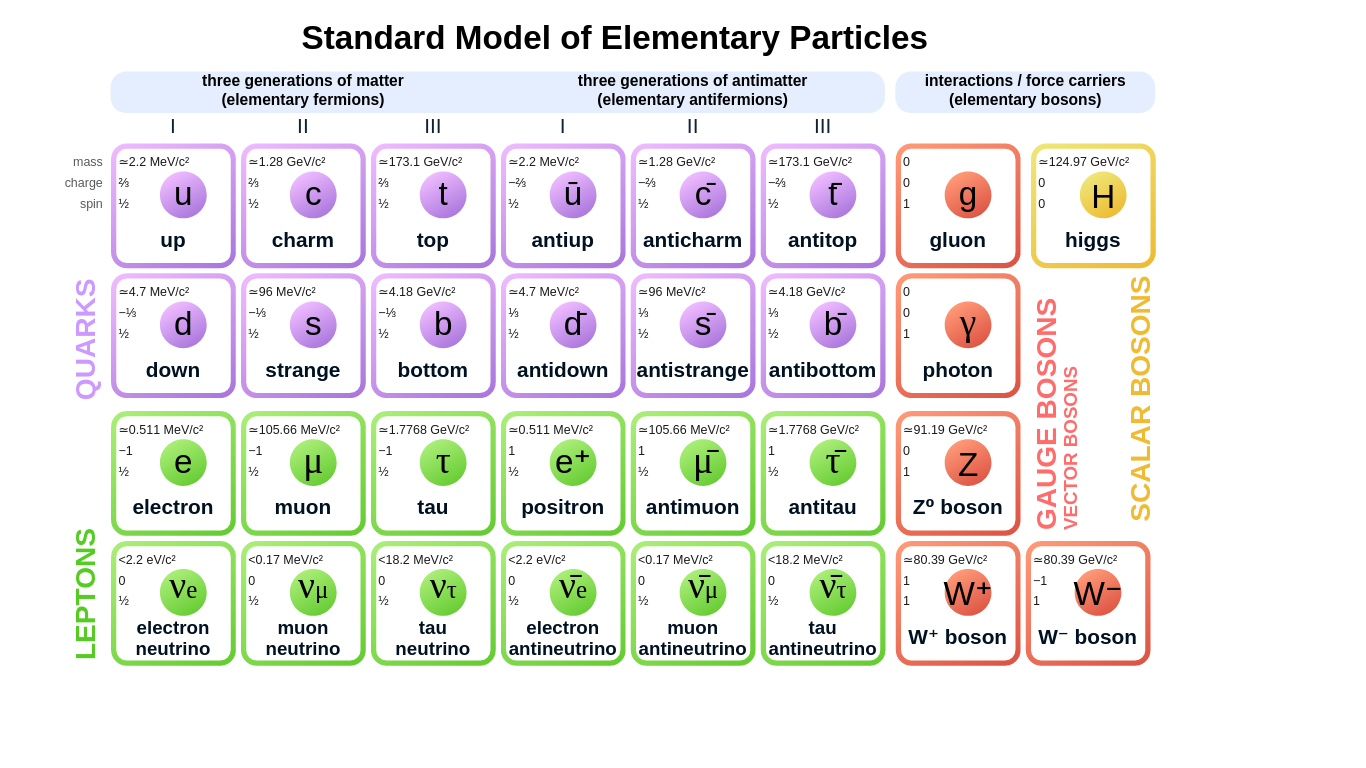
\includegraphics[scale=0.35]{chapter1/sm.png} 
\centering
\caption{Fermions and Bosons in the Standard Model,~figure adopted from~\cite{enwiki:1045150258}.}
\label{Fermions}
\end{figure}

\subsubsection{Bosons}
In standard model, vector bosons~(photons, gluons, graviton, $W$ and $Z$ boson) have integer spin~(spin=1,2) and scaler boson~(Higgs) has no spin~(spin=0). The vector bosons are mediator of interactions~(force) between elementary particles and scaler boson gives mass to other elementary particles. Boson are different from fermions as they obey Bose-Einstein distribution whereas fermions obey Fermi-Dirac distribution. Boson can exist in both states either elementary, like photons, gluons or in a combined state, like mesons.  
\subsubsection{Gluons}
Gluons mediate the strong interaction, which is responsible for the formation of hadrons. The hadrons are of two types, baryons and mesons. Baryon is composed of three quarks and meson has two quarks~(quark-antiquark)  state. Protons and neutrons are baryons, formed by the gluons and form atomic nucleus. Like quarks, gluons have a color and an anti color charge.
\subsubsection{Electroweak Bosons}
Weak bosons are of three types: $W^{+},W^{-},Z^{0}$. These bosons are the mediators of weak interaction. Unlike other bosons these are quite massive. The photon, which is a massless and charge less stable particle, which mediates the electromagnetic interaction. These four bosons are responsible for electroweak~(combined electromagnetic and weak) interaction between fundamental particles.
\subsubsection{Higgs boson}
In the Standard Model, the only massive scalar boson with zero spin is the Higgs boson,~an unstable particle with zero electric charge and no colour charge. Higgs boson decays into other particles almost immediately after it's production. The Higgs boson are the quanta of field called Higgs field which gives mass to elementary particles via mechanism called Higgs mechanism.
\begin{figure}
\centering
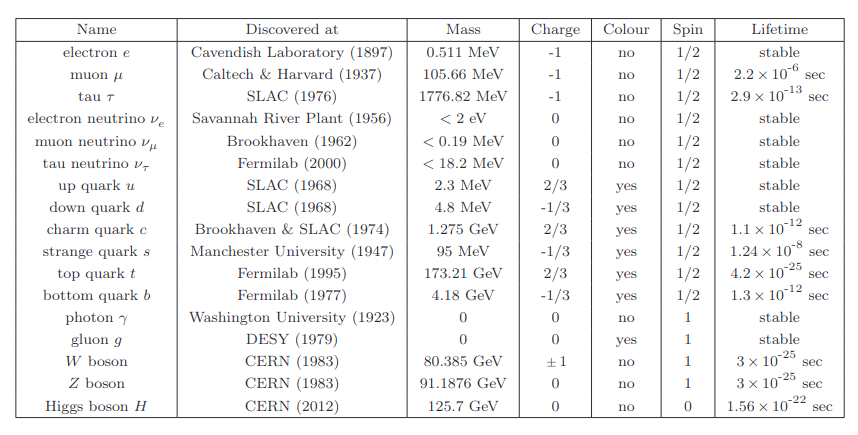
\includegraphics[scale=0.4]{chapter1/particle-sm.png}
\caption{Known Elementary particles in Standard Model. Parameters are taken from ~\cite{ParticleDataGroup:2016lqr}.}
\end{figure}
\section{Beyond Standard Model}
The theoretical predictions that try to explain the shortcomings in SM are referred to as Physics Beyond Standard Model~(BSM). The SM successfully explains particle physics phenomenology in~$\approx$ TeV scale. There are six major question in SM~\cite{Clarke:2016vnr}:
\begin{itemize}
\item Higgs Sector~(What is the nature of electro-weak symmetry breaking?)
\item Naturalness~(Is the mass of Higgs natural?)
\item Neutrino mass~(What is the mechanism by which neutrinos gain mass?)
\item Baryon Asymmetry of the Universe~(How the Universe has more baryons than anti baryons?)
\item Strong CP Problem~(Small neutron electric dipole moment?)
\item Dark Matter~(what is the nature of non-luminous but gravitationally interacting matter?)
\end{itemize}
\subsection{Grand Unification}
The Grand Unification theory~(GUT) predicts that electromagnetic, strong and weak force can merge into a single force at very high energy scale. According to Grand Unified Theory we can merge all three fundamental forces into single one called electro nuclear force. Such unified force can be broken into three fundamental forces by a Higgs like mechanism.  Grand unification models are expected at very high energy scale of about~$\approx 10^{16}~{GeV}$.
\subsection{Supersymmetry~(SUSY)}
Supersymmetry~\cite{article} predicts that each particle in SM either fermion or boson has a partner particle called superpartner. This can help us to explain why particles have mass. Symmetries are very important in modern physics, since they give a nice way to construct Lagrangian for a field or particle from which equation of motion can be found. Well-known examples of symmetries are symmetry under Lorentz transformation, translational symmetry in space-time as well as symmetry under isospin transformations. Supersymmetry is different from these symmetries in that it is invariant under transformation of bosonic field/particle to fermionic field/particle and vice versa. Supersymmetry combines fermionic field and bosonic field in a single field called a super field.\\
There are two class of particles in SM, fermions or bosons based on their spin. All Fermions have $1/2$ units of spin, while the bosons have integer spin~i.e. 0, 1, 2. According to Supersymmetry theory each particle in SM has a partner particle whose spin differs from the particle in integer multiple of 1/2. In this manner Supersymmetry brings two types of SM particles fermions and bosons together.
\subsection{String Theory}
According to String Theory the sub-atomic particles are like a vibrating one dimensional strings rather zero dimensional point particles. The mode of vibration of the string corresponds to the mass, charge and other properties of particle. These strings exist in an eleven dimensional or twelve dimensional universe. These strings can vibrate with different frequencies. These frequencies are responsible for the strings mass, charge and spin. A string can have many shapes, open like a line or closed like a circle or more complicated shapes.
\section{Elementary Particles Dynamics}
There are four fundamental forces in nature through which matter particles interacts with each other. These forces are carried by particles called mediators of force. On the basis of mediating particles these interactions are divided into several types, each one explained below, briefly.


\subsection{Quantum Electrodynamics}
In Quantum Electrodynamics~(QED) the electrically charged particles interact with each other by exchange of fields known as photon.\\
\begin{center}
\feynmandiagram [vertical=a to b] {
i1 [particle=\(e^{-}\)] -- [fermion] a -- [fermion] i2 [particle=\(e^{-}\)],
a -- [photon, edge label=\(q\)] b,
f1 [particle=\(e^{+}\)] -- [fermion] b -- [fermion] f2 [particle=\(e^{+}\)],
};
\end{center}

In above figure time flows horizontally, an electron and positron scattering mediated by a photon is shown. The anti-particle line is always directed backward in time while the particle is going forward. Pair production, Compton scattering and pair annihilation are the fundamental QED processes.  In quantum electrodynamics the force mediators could be photons, electrons or positrons. According the Feynman rule, momentum is conserved at each vertex of Feynman diagram and for the whole process also. \\
\begin{center}
\feynmandiagram [vertical=a to b] {
i1 [particle=\(e^{-}\)] -- [fermion] a -- [anti fermion] i2 [particle=\(e^{+}\)],
a -- [photon, edge label=\(\gamma\), momentum'=\(k\)] b,
f1 [particle=\(\mu^{+}\)] -- [fermion] b -- [anti fermion] f2 [particle=\(\mu^{-}\)],
};\\

\feynmandiagram [horizontal=a to b] {
i1 [particle=\(e^{-}\)] -- [fermion, very thick] a -- [fermion, opacity=0.2] i2 [particle=\(e^{+}\)],
a -- [red, fermion,  momentum'={[arrow style=red]\(k\)}] b,
f1 [particle=\(\gamma\)] -- [boson, opacity=0.2] b -- [boson, very thick] f2 [particle=\(\gamma\)],
};
\end{center}
\subsection{Quantum Chromodynamics}
Quantum chromodynamics is the theory of strong interaction between quarks and gluons, these are the fundamental particle that make up composite particles like hadrons.

Quarks have color charge and can be one of the three color charges red, blue, green. For any fundamental QCD process $q\rightarrow g+q$ the color charge of the quark can change but the flavour remains same. For example in a QCD interaction the color of up~(u) quark may change but its flavour does not change. The color charge is always conserved in any QCD interaction.
In the following Feynman diagram gluon must carry a unit of green and anti blue color charge to ensure color conservation.\\
\begin{center}
\feynmandiagram [horizontal=a to b] {
i1 [particle=\(q(g)\)] -- [fermion] a -- [fermion] i2 [particle=\(q(b)\)],
a -- [gluon, edge label=\(g\bar{b}\)] b,
f1 [particle=\(q(g)\)] -- [anti fermion] b -- [anti fermion] f2 [particle=\(q(b)\)],
};
\end{center}
Gluons have color charge unlike photons which are electrically neutral, thus the gluons can interact with other gluons.\\
The coupling constant for QCD is different from the QED. In QED at each vertex we need a factor of $\alpha$ = 1/137, because this number is very small thus we only need to consider Feynman diagrams with a small number of vertices. QCD coupling constant $\alpha_{s}$ depends upon the separation distance of the interacting particles~(we call it a running coupling constant) at very small distance the value of strong coupling constant become very small, this phenomenon in known as asymptotic freedom. Thus quarks and anti-quarks inside the proton wander like free particles, such behavior was found experimentally in deep inelastic scattering experiments~(DIS). Asymptotic freedom becomes more important in perturbation QCD theory.
\subsection{Weak Interaction}
All quarks and all leptons interact through weak force (leptons have no color charge hence can not interact though strong interaction; neutrinos are charge less, so they cannot interact through electromagnetic forces; but all quarks and leptons can interact through weak interactions.) There are two types of weak interactions: charged weak interactions which are mediated by $W$ boson and weak neutral interactions mediated by neutral $Z$ boson.\\

\begin{center}
\feynmandiagram [horizontal=a to b] {
i1 [particle=\(e^{-}\)] -- [fermion] a -- [fermion] i2 [particle=\(e^{-}\)],
a -- [boson, edge label=\(Z\)] b,
f1 [particle=\(\nu^{\mu}\)] -- [anti fermion] b -- [anti fermion] f2 [particle=\(\nu^{\mu}\)],
};\\

\feynmandiagram [horizontal=a to b] {
  a [particle=\(\mu^{-}\)] -- [fermion] b -- [fermion] f1 [particle=\(\nu_{\mu}\)],
  b -- [boson, edge label=\(W^{-}\)] c,
  f2 [particle=\(e^{-}\)] -- [anti fermion] c -- [fermion] f3 [particle=\(\nu_{e}\)],
};
\end{center}
The interactions in which the mediator is a $Z$ boson is known as neutral weak interaction.\\
The strong, electromagnetic and neutral weak interaction all share the feature that the same quark or lepton comes out when interaction occurs by an exchange of gluon, photon or $Z$ boson. In QCD the color of the quark may change but flavour of particle does not. The charged weak interactions are the only interactions that change flavor of the particles and in this sense they are the only ones capable of causing a true decay.

\begin{center}

\feynmandiagram [vertical=a to b] {
i1 [particle=\(\mu^{-}\)] -- [fermion] a -- [fermion] i2 [particle=\(\nu_{\mu}\)],
a -- [boson, edge label=\(W^{-}\)] b,
f1 [particle=\(\nu_{e}\)] -- [ fermion] b -- [fermion] f2 [particle=\(e^{-}\)],
};
\end{center}

Above Feynman diagram shows weak interaction of leptons in which a negative lepton~($e^{-}, \mu^{-},~\tau^{-}$) converts into the corresponding neutrino mediated by $W^{-}$ boson, $l^{-}\rightarrow\nu_{l}+W^{-}$.
Note in case of weak interaction of leptons, it can only convert into same generation i.e.~$e^{-}$ converts to $\nu_{e},$ and $\mu^{-}\rightarrow\mu^{-}$ with the emission or absorption of $W's$ boson, but $e^{-}$ never convert
into $\mu^{-}$ nor $\mu^{-}$ to $\nu_{e}$. Thus electroweak theory conserves the electron number, muon number, and tau number.

\begin{center}
\feynmandiagram [horizontal=a to b] {
i1 [particle=\(d\)] -- [fermion] a -- [fermion] i2 [particle=\(u\)],
a -- [boson, edge label=\(W^{-}\)] b,
f1 [particle=\(e\)] -- [anti fermion] b -- [fermion] f2 [particle=\(\nu_{e}\)],
};
\end{center}
If a quark interacts with $W^{+}$ boson it will convert into an other quark of same generation~i.e d-quark with charge -1/3 will convert into a u-quark of charge 2/3, similarly for other quarks. In such interactions the flavor of quark changes but color remain same. $W$ and $Z$ bosons also known as Intermediate vector bosons or weak bosons are the mediator of Weak Interactions. They are also called vector bosons due to their spin~(s=1). $W$ bosons have charge $\pm1$ and Z boson is electrically neutral. $W^{+}$ and $W^{-}$ are anti-particles of eachother and $Z$ boson is its own anti-particle. The life time of these bosons is very small with a half-life of about $3\times10^{-25}sec$.  

The $W$ boson is the only one which can cause nuclear transmutation by emission or absorption of leptons. The interaction with the exchange of $Z$ boson is similar to the interactions in QED. $Z$ boson can only transfer momentum or spin between interacting particles. In interaction with exchange of $Z$ boson electrically charged particles can not be emit or absorbed.

The $W$ and $Z$ boson are massive elementary particles with masses $80.4~GeV$~\cite{ddd77f409a1d4f53a9ea8bbf3f2e016d} and $91.2~GeV$~\cite{ddd77f409a1d4f53a9ea8bbf3f2e016d} respectively, due to their high mass range of weak interaction is very small. Photon is the force carrier of Electromagnetic force and has no mass thus EM interactions have infinite range. The hypothetical Graviton also has no mass, Gluons also have no mass but range of strong interaction is not infinite due to the reason called color confinement. 
\subsubsection{Decay of $W$ and $Z$ Boson:}
The $W$ and $Z$ bosons decay into lepton-anti lepton pairs and quark-antiquark pairs but these boson can not decay into top quark because its mass is higher than these bosons. In leptonic decay it decays into charged and neutral leptons and in hadronic decay into a quark and antiquark of different types with opposite electric charge.
The $W$ boson decays leptonically with a branching fraction $\frac{\Gamma_{l}}{\Gamma}= 32.12\%$ and hadronic $\frac{\Gamma_{hadron}}{\Gamma}=67.60\%$~\cite{Wboson}.\\
Similarly $Z$ boson can decay leptonically as well as hadronically with $\frac{\Gamma_{l}}{\Gamma}= 30.7\%$ and $\frac{\Gamma_{hadron}}{\Gamma}=69.2\%$ respectively. The hadronic to leptonic decay ratio for $Z$ boson is $\frac{\Gamma_{hadron}}{\Gamma_{lepton}}=20.767\%$~\cite{Zboson}



\section{Theoretical Overview of Particle Physics}
\subsection{Theory of Quantum Electrodynamics}
The problem with the non-relativistic Schrodinger equation is that,~it has first order derivative of time component and second order derivative of space components. Klein-Gordon used the relativistic energy momentum relation and wrote the Schrödinger equation in a compact way~\cite{Griffith87}.
\begin{equation}\label{KG-equation_free}
(\partial_{\mu}\partial^{\mu}+m^{2})\phi=0,
\end{equation}
In Eq.~\ref{KG-equation_free} $\partial_{\mu}=(\frac{\partial}{\partial(ct)},\overline{\nabla})$ and $\partial^{\mu}=(\frac{\partial}{\partial(ct)},-\overline{\nabla})$ with $\hbar=c=1$.
This Equation represents free particle case. Using Klein-Gordon equation for a wave function $\phi$
\begin{equation}\label{kg-probability density}
\rho=\iota(\phi^{*}\frac{\partial\phi}{\partial t}-\phi\frac{\partial\phi^{*}}{\partial t}),
\end{equation}
\begin{equation}\label{kg-probability current}
J=-\iota(\phi^{*}\nabla\phi-\phi\nabla\phi^{*}),
\end{equation}
The Equation~\ref{kg-probability density} represents probability density and Equation~\ref{kg-probability current} represents probability current.
Consider the plane wave solution for the K-G equation i.e $\phi=N\exp(\iota\overline{p}.\overline{x}\pm\iota Et)$, we get;
\begin{equation}
E=\pm\sqrt{p^{2}+m^{2}},
\end{equation}

\begin{equation}
\rho=2E|N|^{2},
\end{equation}
The problem with K-G equation is that it has negative energy solutions~($E<0$) and similarly with the probability density.

\subsubsection{Dynamics of Photon}
In electrodynamics, charge density $\rho$ and current density $J$ of electromagnetic field are determined by Maxwell's equations in vaccum, where $\overline{E}$ is the electric field and $\overline{B}$ is the magnetic field,
\begin{equation}
\overline{\nabla}.\overline{E}=\frac{\rho}{\epsilon_{0}},
\end{equation}
\begin{equation}
\overline{\nabla}\times\overline{E}=-\frac{\partial{\overline B}}{\partial{t}},
\end{equation}
\begin{equation}
\overline{\nabla}.\overline{B}=0,
\end{equation}
\begin{equation}
\overline{\nabla}\times\overline{B}=\overline{J}+\frac{\partial\overline{E}}{\partial t},
\end{equation}
The electric and magnetic fields in terms of an electromagnetic potential are given as,
\begin{equation}~\label{E_field}
\overline{E}=-\overline{\nabla}\phi-\frac{\partial{\overline{A}}}{\partial t},
\end{equation}
\begin{equation}\label{B_field}
\overline{B}=\overline{\nabla}\times\overline{A},
\end{equation}
In relativistic notation,the field tensor for $\overline{E}$ and $\overline{B}$, $F^{\mu\nu}$~\cite{Griffith-ed} is,

\begin{center}
$F^{\mu\nu}$~=~$\begin{pmatrix}
0 & -E_{x} & -E_{y} & -E_{z}\\
E_{x} & 0 & -B_{z} & B_{y}\\
E_{y} & B_{z} & 0 & -B_{x}\\
E_{z} & -B_{y} & B_{x} &0\\
\end{pmatrix}$
\end{center}
The inhomogeneous Maxwell equations can be written In terms of field tensor:
\begin{equation}
\partial_{\mu}F^{\mu\nu}~=~J^{\nu},
\end{equation}
and similarly for homogeneous Maxwell equations:
\begin{equation}
\partial_{\mu}\tilde{F}^{\mu\nu}~=~0,
\end{equation}
The $\tilde{F}^{\mu\nu}$ is called dual or antisymmetric field tensor. The Equations \ref{E_field} and \ref{B_field} can be written in relativistic notation:
\begin{equation}
F^{\mu\nu}~=~\partial^{\mu}A^{\nu}-\partial^{\nu}A^{\mu},
\end{equation}
here $A^{\mu}~=~(\phi,\overline{A})$ is the four vector potential. In terms of four vector potential the inhomogeneous Maxwell Equations can be written :
\begin{equation}
J^{\nu}~=~\partial_{\mu}.\partial^{\mu}A^{\nu}-\partial^{\nu}.\partial_{\mu}A^{\mu},
\end{equation}
In the potential formulation we can not uniquely determine $V$~(scalar potential) and $A$~(vector potential). So we transform $A^{\mu}$:
\begin{equation}
\grave{A}^{\mu}~=~A^{\mu}+\partial^{\mu}\chi,
\end{equation}
This transformation $\grave{A}^{\mu}~=~A^{\mu}+\partial^{\mu}\chi$ is called gauge transformation and $\overline{E}$ and $\overline{B}$ fields remain invariant under gauge transformation. Here $\chi$ is some scalar function of position and time. The freedom to choose any $\grave{A}^{\mu}=A^{\mu}+\partial^{\mu}\chi$ is called gauge freedom. The gauge condition can be applied to potential in the following way:
\begin{equation}
\partial_{\mu}A^{\mu}~=~0,
\end{equation}
called Lorentz condition, Maxwell equations with this Lorentz condition applied become:
\begin{equation}
\partial_{\mu}\partial^{\mu}A^{\nu}~=~J^{\nu},
\end{equation}
Maxwell equation with Lorentz gauge condition is applied. For the empty space  $J^{\nu}~=~0$ and Maxwell equation reduces to,
\begin{equation}\label{massless_photon}
\partial_{\mu}\partial^{\mu}A^{\nu}~=~0,
\end{equation}
this equation is recognised as Klein-Gordon equation for massless particles. In QED $A^{\nu}$ is the wave function of free photon, and plane wave solution for the massless photons are given by,
\begin{equation}
A^{\nu}~=~a\epsilon^{\nu}(p) e^{-\iota\overline{p}.\overline{x}},
\end{equation}

Here $\epsilon^{\nu}$ is polarization vector, by substituting this solution into Equation\ref{massless_photon} we get 
\begin{equation}
P^{\mu}P_{\mu}=0,~E~=~pc,
\end{equation}
which should be true for massless particles.
Lorentz condition $\partial_{\mu}A^{\mu}~=~0$ requires that 
\begin{equation}
P^{\mu}\epsilon_{\mu}~=~0
\end{equation}
In the Coulomb's gauge 
\begin{equation}
\epsilon^{0}~=~0
\end{equation}
These equations show that the polarization vector of photon ($\epsilon$) is perpendicular to the direction of propagation; if the direction of propagation is $z-axis$, then photon will be polarized in $xy-axis.$, thus we have only two linearly independent vectors perpendicular to $\overline{p}$; for example, if $\overline{p}$ is in the $z$ direction, we might choose;
\begin{eqnarray}
\epsilon^{1}=(1,0,0)\\
\epsilon^{2}=(0,1,0)
\end{eqnarray}
A particle with mass have $2s+1$ spin directions and massless particle has only two, independent of its spin, along its direction of motion it can only have $m_{s}~=~+s   $  or $m_{s}~=~-s$.

\subsubsection{Dynamics of Spin 1/2 Particles}
The problem with Schrodinger equation is that it cannot explain the dynamics of relativistic particles because it is quadratic in space or position coordinate but first order derivative of time parameter, and problem with the Klein-Gordon equation is that, it cannot explain the dynamics of spin 1/2 particles. To address these problems Dirac introduced Dirac equation~\cite{diracequation}.
It was known that;
\begin{equation}
H^{2}\psi~=~(\overline{p}^{2}+m^{2})\psi,
\end{equation} 
Dirac introduced;
\begin{equation}
H\psi~=~(\overline{\alpha}.\overline{p}+\beta m)\psi,
\end{equation}
Here $\alpha$ and $\beta$ are matrices with the following properties;
\begin{enumerate}
\item Eigen values~=~$\pm1$.
\item Trace~=~0.
\item$\alpha_{i},\beta$ are hermitian matrices.
\item All matrices are linearly independent.
\end{enumerate}
Thus $4\times4$ is the minimum number of  dimensions required for the Dirac matrices. Dirac matrices may be written as;
\begin{center}
$\overline{\alpha}_{i}$=$\begin{pmatrix}
0 & \overline{\sigma}_{i}\\
\overline{\sigma}_{i} & 0

\end{pmatrix}$,\\
\end{center}
\begin{center}
$\beta$=$\begin{pmatrix}
\mathbf{1} & 0\\
0 & \mathbf{1}
\end{pmatrix}.$
\end{center}
here $\overline{\sigma}_{i}$ are the $2\times 2$ Pauli matrices, we can write Dirac matrices in standard notation;
\begin{equation}
\gamma^{\mu}=(\beta,\beta\overline{\alpha});
\end{equation}
here $\gamma^{0}=\beta,\gamma^{1}=\beta\alpha_{1},\gamma^{2}=\beta\alpha_{2}$ and $\gamma^{3}=\beta\alpha_{3}$.
Dirac equation in compact notation may be written as
\begin{equation}\label{Dirac equation}
(\iota\gamma^{\mu}\partial_{\mu}-m)\psi=0.
\end{equation}
\subsubsection{Plane Wave Solution of Dirac Equation}
For a particle at rest $p=0$;~\footnote{for detail see:David Griffith's Introduction to elementary particles(second revised edition),Section 7.2}
\begin{eqnarray}
\psi_{A}(t)=e^{-\iota(\frac{mc^{2}}{\hbar})t}\psi_{A}(0),\\
\psi_{B}(t)=e^{\iota(\frac{mc^{2}}{\hbar})t}\psi_{B}(0),
\end{eqnarray}
Where $\psi_{A}$ represents a particle with positive energy and $\psi_{B}$ represents a particle with negative energy.
Here $\psi_{A}$=$\begin{pmatrix}
\psi_{1}\\
\psi_{2}
\end{pmatrix}$
and $\psi_{B}$=$\begin{pmatrix}
\psi_{3}\\
\psi_{4}
\end{pmatrix}$\\
when $p\neq0$;
\begin{eqnarray}
\psi=a e^{-\iota\frac{p.x}{\hbar}}u,\\
\psi=a e^{\iota\frac{p.x}{\hbar}}v,
\end{eqnarray}
here $u$ and $v$ are Dirac four dimensional spin matrices.
\subsubsection{Interacting Charged Fermions}
Dirac equation for free a particle:\footnote{For detail see: chapter six of Quarks and Leptons:An introductory Course by Francis Halzen and Alan D.Martin}
\begin{eqnarray}
(\gamma^{\mu}p_{\mu}-m)\psi=0,\\
(\gamma^{0}p_{0}-\overline{\gamma}.\overline{p}-m)\psi=0,\\
E\psi=(\gamma^{0}\overline{\gamma}.\overline{p}+m\gamma^{0})\psi,
\end{eqnarray}
For Interaction:
\begin{equation}
p^{\mu}\rightarrow p^{\mu}-QA^{\mu},
\end{equation}
for the case of electron
\begin{equation}
p^{\mu}\rightarrow p^{\mu}+eA^{\mu},
\end{equation}
so the Dirac equation for an electron interacting with E-M field~($A^{\mu}$)\\

\begin{eqnarray}
\gamma^{\mu}(p_{\mu}+eA_{\mu})\psi-m\psi=0,\\
E\psi=(\gamma^{0}\overline{\gamma}.\overline{p}+m\gamma^{0})\psi-e\gamma^{0}\gamma^{\mu}A_{\mu}\psi,
\end{eqnarray}
here 

\begin{equation}\label{dirac_potential}
V= e\gamma^{0}\gamma^{\mu} A_{\mu} \psi.
\end{equation}
The potential for an electron interacting with EM field. The transition amplitude for the electron from state $\psi_{i}$ to $\psi_{f}$ is 
\begin{equation}\label{Transition_amp}
T_{fi}=-\iota\int\psi_{f}^{\dagger}V\psi_{i}d^{4}x,
\end{equation}
By putting the value in Eq.~\ref{Transition_amp} from Eq.~ \ref{dirac_potential} we get:

\begin{equation}\label{Tfi}
T_{fi}=-\iota\int J^{\mu}A_{\mu}d^{4}x,
\end{equation}
here $J^{\mu}$ is four vector current:
\begin{equation}
J^{\mu}=-e\psi^{*}\gamma^{\mu}\psi,
\end{equation}
and $A_{\mu}$ is the E-M potential through which electron interacts. The source field $A_{\mu}$ must satisfy the equation
\begin{equation}
\partial_{\mu}\partial^{\mu}A^{\mu}=j^{\mu},
\end{equation}
and its solution is 
\begin{equation}
A^{\mu}=-\frac{1}{q^{2}}j^{\mu},
\end{equation}
Now Equation~\ref{Tfi} become 
\begin{equation}\label{Transition}
T_{fi}=-\iota\int J_{1}^{\mu}(-\frac{g_{\mu\nu}}{q^{2}})J_{2}^{\nu}d^{4}x,
\end{equation}
\begin{center}
\feynmandiagram [horizontal=a to b] {
i1 [particle=\(J_{1}^{\mu}(P_{A})\)] -- [fermion] a -- [fermion] i2 [particle=\(J_{1}^{\mu}(P_{C})\)],
a -- [photon, edge label=\(-\frac{g_{\mu\nu}}{q^{2}}\)] b,
f1 [particle=\(J_{2}^{\nu}(P_{D})\)] -- [anti fermion] b -- [anti fermion] f2 [particle=\(J_{2}^{\nu}(P_{B})\)],
};
\end{center}
The above Feynman diagram represents electron-electron interaction,in which photon is a mediator of force.\\
\begin{equation}\label{j1}
J_{1}^{\mu}=-e \psi_{B}^{*}\gamma^{\mu}\psi_{A},
\end{equation}
\begin{equation}\label{j2}
J_{2}^{\nu}=-e \psi_{D}^{*}\gamma^{\mu}\psi_{C},
\end{equation}
By substituting Equations~\ref{j1} and~\ref{j2} in~\ref{Transition} we get:
\begin{eqnarray}
T_{fi}=-\iota(2\pi)^{4}\delta^{4}(P_{A}+P_{c}-P_{B}-P_{D}).\mathcal{M},\\
\mathcal{M}=(-e\overline{U}_{B}\gamma^{\mu}U_{A})(-\frac{g_{\mu\nu}}{(p_{A}-p_{B})^2})(-e\overline{U}_{D}\gamma^{\mu}U_{C}),
\end{eqnarray}

$\mathcal{M}$ is called "Lorentz Invariant Transition Amplitude"

\textbf{Example}( we may write electron-muon scattering amplitude as:)\\
\begin{center}
\feynmandiagram [horizontal=a to b] {
i1 [particle=\(p(1)e\)] -- [fermion] a -- [fermion] i2 [particle=\(p(3)e\)],
a -- [photon, edge label=\(q\)] b,
f1 [particle=\(p(2)\mu\)] -- [anti fermion] b -- [anti fermion] f2 [particle=\(p(4)\mu\)],
};
\end{center}

By following Feynman rules we can write out Scattering amplitude~($\mathcal{M}$ for the above diagram):
\begin{equation}
\mathcal{M}=-\frac{g_{e}^{2}}{(p_{1}-p_{3})^{2}}[\overline{u}_{3}(p_{3})\gamma^{\mu}u_{1}(p_{1})][\overline{u}_{4}(p_{4})\gamma_{\mu}u_{2}(p_{2})]
\end{equation}
\subsection{Theory of Quantum Chromodynamics}
Quantum electrodynamics~(QED) explains the interaction between charged particles; Quantum chromodynamics~(QCD) describes the interaction between coloured particles; The mediator of electromagnetic interactions are photon and strong interactions are mediated by gluons which also massless particle. The coupling constant for the electromagnetic interaction is given by
\begin{equation}
g_{e}=\sqrt{4\pi\alpha}
\end{equation}
and coupling constant for the strong force is set by strong coupling constant
\begin{equation}
g_{s}=\sqrt{4\pi\alpha_{s}}
\end{equation}

Quarks can be labeled with different colour quantum number, red~(r), blue~(b) and green~(g), therefore to describe the colour of quarks we must have an additional term in the Dirac spinor which gives the colour factor of these quarks.
For red:
\begin{equation}
c=\begin{pmatrix}
1\\
0\\
0
\end{pmatrix}
\end{equation}
for blue:
\begin{equation}
c=\begin{pmatrix}
0\\
1\\
0
\end{pmatrix}
\end{equation}
and for green:
\begin{equation}
c=\begin{pmatrix}
0\\
0\\
1
\end{pmatrix}
\end{equation}

Each gluon carries one unit of colour and one unit of anti-colour then, there should be nine species of gluons. In term of SU(3) symmetry these nine states constitutes a 'colour octet' and a 'colour singlet'.\footnote{For detail see chapter 8 of 'Introduction to Elementary Particles' by David Griffith's}
Gluons are also massless spin 1 particles; similarly as for the photon, $\epsilon^{\mu}$ is the polarisation vector of gluon which is perpendicular to the momentum of gluon:
\begin{equation}
\epsilon^{\mu}p_{\mu}=0
\end{equation}

And Coulomb gauge condition gives

\begin{equation}
\epsilon^{0}=0
\end{equation}

\subsubsection{Quark anti-quark Interaction}
In quark and an antiquark interaction, both have different flavors, the interaction amplitude is given by:
\begin{center}
\feynmandiagram [vertical=a to b] {
i1 [particle=\(p(1)c(1)\)] -- [fermion] a -- [fermion] i2 [particle=\(p(3)c(3)\)],
a -- [photon, edge label=\(q\)] b,
f1 [particle=\(p(4)c(4)\)] -- [fermion] b -- [fermion] f2 [particle=\(p(2)c(2)\)],
};
\end{center}

\begin{equation}
\mathcal{M}=\iota[\overline{u}(3)c_{3}^{\dagger}](-\iota\frac{g_{s}}{2} \lambda^{\alpha}\gamma^{\mu})[u(1)c_{1}](\frac{\iota g_{\mu\nu}\delta_{\alpha\beta}}{q^{2}})\times[\overline{\nu}(2)c_{2}^{\dagger}](-\iota\frac{g_{s}}{2} \lambda^{\beta}\gamma^{\nu})[\nu(4)c_{4}]
\end{equation}
Thus

\begin{equation}
\mathcal{M}=-\frac{g_{s}^{2}}{4q^{2}}[\overline{u}(3)\gamma^{\mu}u(1)][\overline{\nu}(2)\gamma_{\nu}\nu(4)][c_{3}^{\dagger}\lambda^{\alpha}c_{1}][c_{2}^{\dagger}\lambda^{\alpha}c_{4}]
\end{equation}


Here $g_{e}$ is replaced by $g_{s}$, and the extra term, which is called color factor.\\
\begin{center}
$f=\frac{1}{4}(c_{3}^{\dagger}\lambda^{\alpha}c_{1})(c_{2}^{\dagger}\lambda^{\alpha}c_{4})$
\end{center}
The color factor for the octet configuration is -1/6 and for the singlet configuration is -4/3. Thus the quark-antiquark potential are
\begin{center}
$V_{q\overline{q}}=-\frac{4\alpha_{s}\hbar c}{3r}$\\
$V_{q\overline{q}}=\frac{\alpha_{s}\hbar c}{6r}$
\end{center}
for color singlet and color octet configuration respectively. 

\subsubsection{Quark Quark Interaction}
For the interaction between quark-quark the invariant amplitude can be written as:
\begin{equation}
\mathcal{M}=-\frac{g_{s}^{2}}{4q^{2}}[\overline{u}(3)\gamma^{\mu}u(1)][\overline{u}(4)\gamma_{\mu}u(2)][c_{3}^{\dagger}\lambda^{\alpha}c_{1}][c_{4}^{\dagger}\lambda^{\alpha}c_{2}],
\end{equation}

The colour factor for this interaction is given by:
\begin{center}
$f=\frac{1}{4}(c_{3}^{\dagger}\lambda^{\alpha}c_{1})(c_{4}^{\dagger}\lambda^{\alpha}c_{2})$
\end{center}
The color factor for the triplet configuration is -2/6 and for the sextet configuration is 1/3. Thus the quark-antiquark potential
\begin{center}
$V_{q\overline{q}}=-\frac{2\alpha_{s}\hbar c}{3r}$,\\
$V_{q\overline{q}}=\frac{\alpha_{s}\hbar c}{3r}$,
\end{center}
for color triplet and color sextet configuration respectively. 

\subsubsection{Asymptotic Freedom}
In QED, the electron charge is directly related to momentum transfer of the interaction $q$.~\footnote{Equation 8.91 'introduction to Elementary Particles' by David Griffith's }
In QCD the running coupling constant is
\begin{equation}\label{alpha1}
\alpha_{s}(q^{2})=\frac{\alpha_{s}(\mu^{2})}{1+[\frac{\alpha_{s}(\mu^{2})}{12\pi}](11n-2f)\ln(\frac{q^{2}}{\mu^{2}})},
\end{equation}
here $n$ is the number of color(3) and $f$ is the number of flavour(6). $\alpha_{s}$ is inversely proportional to $q^{2}$ and at short distance or high $q^{2}$ the $\alpha_{s}$ becomes very small and the strong force becomes relatively weak, this is also called asymptotic freedom.
The coupling strength increase as we increase the distance between two
quarks~(antiquarks) and strong force becomes very large. If we try to
separate two quarks then new quark-antiquark pairs are formed and process
of hadronisation occurs. That's why the quarks are always confined inside hadrons and phenomenon is called “quark confinement”, that is why no single quark or gluon could be observed.
In QCD long distance or low $q^{2}$~i.e.~$q^{2}=0$ is not allowed, because at this scale $\alpha_{s}$ becomes very large, and perturbative QCD calculation can not be applied. For QCD perturbation expansions, we must set a reference scale where $\alpha_{s}$ is small enough that perturbative expansion can be done. Equation~\ref{alpha1} is expressed in term of $\alpha_{s}(\mu^{2})$ so that  $\alpha_{s}(\mu^{2})<< 1$, the running coupling constant can be expressed in terms of a
single parameter:
\begin{equation}
\alpha_{s}(q^{2})=\frac{12\pi}{(11n-2f)ln(\frac{q^{2}}{\Lambda^{2}})}  (q^{2}>>\Lambda^{2}),
\end{equation}
\subsubsection{Running Coupling}
The coupling strength for QED, QCD and Electro weak~(EW) processes are energy scale dependent. The pair production of electrically charged virtual particles leads to vacuum polarisation around charged fermions and consequently a distance-dependent shielding of their fundamental electric charge. This causes running coupling constant $g_{e}$ to increase with the energy scale of the interaction $q^{2}$, and decreasing length-scale. The running of QCD and EW coupling constants follow the opposite trend, at least up to the symmetry breaking scale. The equivalent effect for colour charge, quark pair production and gluon self-coupling contributions (cubic and quartic), effect the range of QCD interactions. If as in nature, $2N_{f}-11N_{c}\neq 0$ $(N_{f} = 6, N_{c} = 3)$ then quarks will experience asymptotic freedom such that $g_{s}$ increases with length-scale and with decreasing $Q^{2}$. As a result of the running of the strong coupling strength, at low energies $q^{2}$ the perturbative approximation are invalid. The bare quarks will produce $qq$ pairs from the vacuum to exist as colour charge-neutral states in a process known as confinement. These colourless states are known as hadrons which include $q\overline{q}$ (mesons) and $qqq$/$ \overline{q}\overline{q}\overline{q}$(baryons)
\begin{figure}
\centering
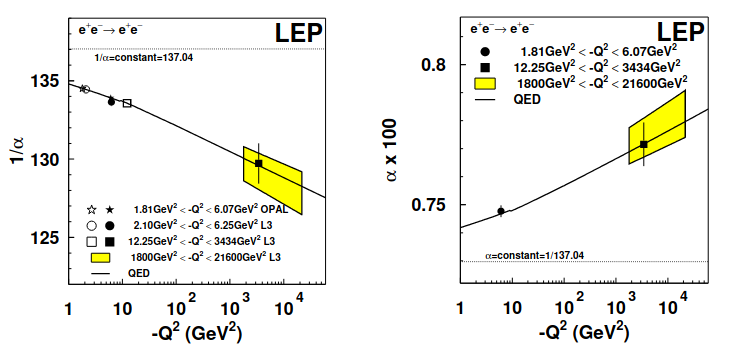
\includegraphics[scale=0.5]{chapter1/alphas1.png}
\caption{Trend of QED running coupling constant with $Q^{2}$~(left), QCD running coupling constant with $Q^{2}$~(right),~figure adopted from~\cite{ACHARD200526}.}
\end{figure}
\begin{figure}[h!]
\centering
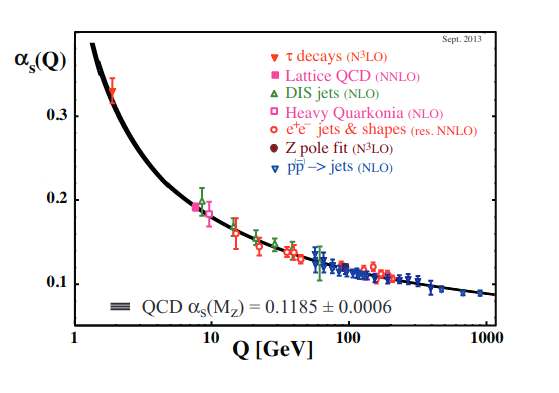
\includegraphics[scale=0.6]{chapter1/alphs1.png}
\caption{The change in the vale of $\alpha_{S}$ with the energy scale Q and the current world average value is illustrated,~Figure taken from~\cite{denterria2015highprecision}}
\end{figure}

\subsection{Theory of Weak Interactions}
Weak interaction are mediated by (as photons for QED and gluons for QCD) the $W$ and $Z^{0}$ bosons and these mediators are extremely heavy. Experimentally $M_{w}=80.387~\pm~0.016~GeV$~\cite{PhysRevD.98.030001} and $M_{z}=91.188~\pm~0.0031~GeV$~\cite{PhysRevD.98.030001}.

We know that the massless photons and gluons have two polarization states after imposing Lorentz condition and Coulomb gauge condition but particles with mass and spin one, are allowed to have three polarization states~$m_{s}=(-1,0,1)$, Thus for the $W$ and $Z$ boson the completeness relation is quite different and propagator factor no longer remain same but becomes,$\frac{\iota g_{\mu\nu}}{Mc^{2}}$ here we assume $q^{2}<<(Mc^{2})$.
\subsubsection{Charged Weak Interaction}
\begin{center}
\feynmandiagram [vertical=a to b] {
i1 [particle=\(e(p1)\)] -- [fermion] a -- [fermion] i2 [particle=\(\nu_{e}p(3)\)],
a -- [boson, edge label=\(W\)] b,
f1 [particle=\(\mu p(4)\)] -- [anti fermion] b -- [anti fermion] f2 [particle=\(\nu_{\mu}p(2)\)],
};
\end{center}
Considered the process,
$\nu_{\mu}+e^{-}\rightarrow\mu^{-}+\nu_{e}$
The amplitude for this interaction is
\begin{equation}
\mathcal{M}=\frac{g_{W}^{2}}{8(M_{w}c^{2})}[\overline{u}(3)\gamma^{\mu}(1-\gamma^{5})u(1)][\overline{u}(4)\gamma_{\mu}(1-\gamma^{5})u(2)],
\end{equation}
Here $\gamma^{\mu}$ alone represents vector coupling whereas $\gamma^{\mu}\gamma^{5}$ would be an axial vector. When we mix a vector to an axial vector then we are bound to violate the parity conservation, that is what happens in weak interactions. Here $g_{w}=\sqrt{4\pi\alpha_{w}}$ and its value is 0.653, and hence the weak fine structure constant is $\alpha_{w}=\frac{1}{29.5}$. This coupling constant is roughly 5 times larger than that of QED but weak interaction are feeble because of massive mediators $W$ and $Z$ bosons.

\subsubsection{Decay of Neutron}
\begin{center}
\feynmandiagram [vertical=a to b] {
i1 [particle=\(n(p1)\)] -- [fermion] a -- [fermion] i2 [particle=\(p(p3)\)],
a -- [boson, edge label=\(W\)] b,
f1 [particle=\(e(p4)\)] -- [anti fermion] b -- [fermion] f2 [particle=\(\nu_{e}(p2)\)],
};
\end{center}

The above Feynman diagram shows the beta decay of neutron, by applying Feynman calculus we find that the neutron life time $\tau=\frac{1}{\Gamma}=1318~s$, as the experimental neutron lifetime is $885.7\pm0.8$~\cite{serebrov2019neutron} seconds. The problem arises due to fact that we treat the proton and neutron as a point particles like leptons, which interact with the $W$ boson. We don't know, what kind of structure protons and neutrons have and what kind of interactions are going on inside proton~i.e.~(valence quarks interaction with gluon, quark pairs formed by gluons, hadronisation) but all  the finalized activity conserves charge. This problem arises becuse we don't know how quarks couple with the vector bosons.
\subsubsection{Neutral Weak Interaction}
\begin{center}
\feynmandiagram [vertical=a to b] {
i1 [particle=\(e(p1)\)] -- [fermion] a -- [fermion] i2 [particle=\(e(p3)\)],
a -- [boson, edge label=\(Z\)] b,
f1 [particle=\(\overline{\nu}_{\mu}(p4)\)] -- [fermion] b -- [fermion] f2 [particle=\(\overline{\nu}_{\mu}(p2)\)],
};
\end{center}

The above Feynman diagram shows $\overline{\nu_{\mu}}+e\rightarrow\overline{\nu_{\mu}}+e$ process mediated by $Z$ boson.
The vertex factor for the $Z^{0}$ boson is not so simple;
\begin{equation}
\frac{-\iota g_{z}}{2}\gamma^{\mu}(c_{v}^{f}-c_{A}^{f}\gamma^{5})
\end{equation}

Where $g_{z}$ is the neutral coupling constant, and the coefficient, $c_{v}^{f}$ and $c_{A}^{f}$ depend on the particular quark or lepton involved. All these parameters are determined by single parameter called $\theta_{W}$ the 'weak mixing angle'. The weak and electromagnetic coupling constant are related:
\begin{equation}
g_{e}=\frac{g_{e}}{sin\theta_{w}},    g_{z}=\frac{g_{e}}{sin_{\theta_{w}}cos_{\theta_{w}}}
\end{equation}
The experimental value of $\theta_{w}$ is 28.75. The amplitude for the above scattering at low energies~($q^{2}<<M_{z}^{2}c^{2}$) is:
\begin{equation}
\mathcal{M}=\frac{g_{z}^2}{8(M_{Z}c)^2}[\overline{u}(3)\gamma^{\mu}(1-\gamma^{5})u(1)][\overline{u}(4)\gamma_{\mu}(c_{v}-c_{A}\gamma^{5})u(2)]
\end{equation}\\

\section{Gauge Symmetry}
The lagrangian densities for the fermionic and electromagnetic fields can be written~\cite{Quarks&lepton87}\\
K-G equation:
\begin{equation}
\mathcal{L}=\frac{1}{2}(\partial_{\mu}\phi)(\partial^{\mu}\phi)-\frac{1}{2}m^{2}\phi^{2},
\end{equation}
Dirac equation:
\begin{equation}
\mathcal{L}=\iota\overline{\psi}\gamma^{\mu}\partial_{\mu}\psi-m\overline{\psi}\psi,
\end{equation}
Maxwell equation:
\begin{equation}
\mathcal{L}=\frac{-1}{4}F^{\mu\nu}F_{\mu\nu}-j^{\mu}A_{\mu},
\end{equation}

Now if we transform the field $\psi$ of the Dirac Lagrangian as $\psi\rightarrow\psi^{\prime}=e^{\iota\alpha}\psi$ where $\alpha$ is some constant. Such transformation of field is called Global gauge transformation and Lagrangian $\mathcal{L}$ remains invariant under such transformation.
To make the Lagrangian invariant under local gauge transformation $\psi\rightarrow\psi^{\prime}=e^{\iota\alpha(x)}\psi$ we have to introduce an extra term in the Dirac Lagrangian which corresponds to electromagnetic interaction and the Lagrangian becomes:
\begin{equation}
\mathcal{L}=\iota\overline{\psi}\gamma^{\mu}\partial_{\mu}\psi-m\overline{\psi}\psi+\frac{-1}{4}F_{\mu\nu}F^{\mu\nu}-j^{\mu}A_{\mu},
\end{equation}


\subsubsection{Higgs Mechanism and Higgs Boson}

The electromagnetic and weak force can be described with the same theory, thus with this unification we can say that electromagnetic and weak forces can be treated as a single force known as the electroweak force.

The unification theory correctly explains the electromagnetic and weak field and associated force carrying particles but the problem is, according to this theory all the mediators are massless but $W$ and $Z$ bosons have mass up to  100 times of mass of proton. The theory which solve this puzzle is called Higgs mechanism. Which says that $W$ and $Z$ bosons acquire mass with the interaction of invisible field called Higgs field.

To understand the electroweak interaction we have to construct Lagrangian that is invariant under the $SU(2)\times U(1)$ transformation.
But we know that $W$ and $Z$ bosons are massive and with the mass term in Electro-weak Lagrangian we must break the gauge invariance. We can write the Lagrangian for weak interaction~\footnote{For detail see chapter 14 of Quarks and Lepton: An introductory course in Modern physics by Francis Halzen Alan D.Martin}:
\begin{equation}
\mathcal{L}=\overline{\psi}\iota\gamma^{\mu}\partial_{\mu}\psi+\iota\frac{f}{2}\tau.W_{\mu}\psi-\frac{1}{4}W_{\mu\nu}W^{\mu\nu},
\end{equation}
here the last term corresponds to weak field tensor.

But we need mass for the $W$ and $Z$ boson and with the mass term Lagrangian is no more gauge invariant, so we have to break the gauge symmetry. So together with mass term in Lagrangian along with gauge symmetry we introduce a Lagrangian:
\begin{equation}
\mathcal{L}=\frac{-1}{4}B_{\mu\nu}B^{\mu\nu},
\end{equation}
where $B_{\mu\nu}=\partial_{\mu}B^{\mu}-\partial_{\nu}B^{\mu}$ and it transforms like $A^{\mu}$
\begin{equation}
B^{\mu}\rightarrow B^{\prime}{\mu}=B^{\mu}+\partial^{\mu}\Lambda,
\end{equation}
where $\Lambda$ is some scalar function and $B^{\mu}$ is some vector field. The Lagrangian becomes:
\begin{equation}
\mathcal{L}=\frac{-1}{4}B_{\mu\nu}B^{\mu\nu}+\mathcal{L}_{scaler},
\end{equation}
\begin{equation}
\mathcal{L}_{scaler}=(D_{\mu}\phi)^{*}(D^{\mu}\phi)-V(\phi^{*}\phi),
\end{equation}

\begin{equation}
D_{\mu}=\partial^{\mu}-\iota gB^{\mu},
\end{equation}
and $\phi$ is some complex field given by $\phi(x)=e^{\iota\phi(x)}(\frac{v+h(x)}{\sqrt{2}})$,and $B^{\mu}\rightarrow B^{\prime\mu}=B^{\mu}+\frac{1}{g}.\partial^{\mu}\theta$ Now  If we make a gauge transformation
\begin{equation}
\phi\rightarrow\phi^{\prime}=e^{i\theta}.\phi,
\end{equation}
\begin{equation}
B_{\mu}\rightarrow B_{\mu}^{\prime}=B_{\mu}+\frac{1}{g}\partial^{\mu}\theta,
\end{equation}
we also have a mass term in the Lagrangian which can be written as:
\begin{equation}
M_{B}=\frac{g^{2}v^{2}}{2},
\end{equation}
and energy term:
\begin{equation}
V=\lambda(\phi^{*}\phi-\frac{v^{2}}{2})^{2},
\end{equation}
thus for minimum energy of scalar field $\phi$ by setting $\frac{\partial v}{\partial \phi}=0$ we get:
\begin{equation}
<\phi>=\begin{pmatrix}
0\\
\frac{V}{\sqrt{2}}
\end{pmatrix}
\end{equation}


corresponds to vacuum. This means when we say vacuum we don't have presence of physical particles or physical fields. Then quantum fluctuation or particles can be created by  giving energy greater than $<\phi>$. Thus presence of $<\phi>$~(Higgs field) gives the mass $M_{B}$ through the interaction of $B_{\mu}$ field with $\phi$ Higgs field.
\begin{figure}[h!]
\begin{tabular}{cc}
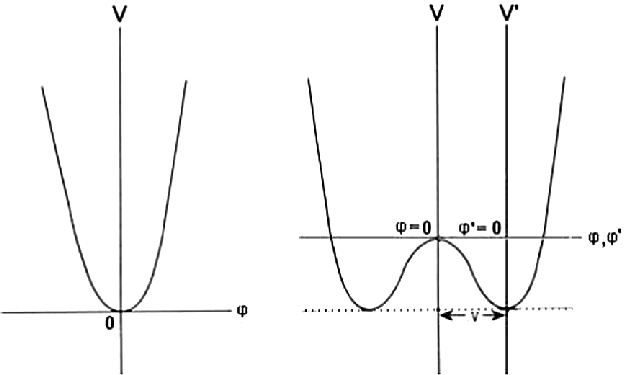
\includegraphics[scale=0.3]{chapter1/Symmetry breaking.png}
&
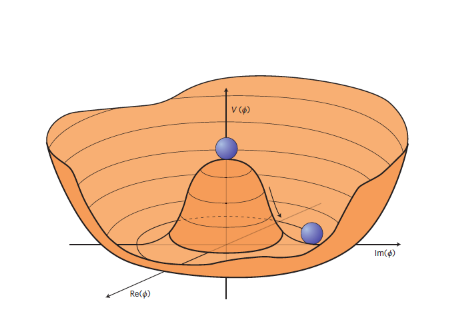
\includegraphics[scale=0.5]{chapter1/sym_break.png}
\end{tabular}

\caption{The potential V of a complex scaler field $\phi$~\cite{Ellis_2016}}
\end{figure}
The physical particles that corresponds to $\phi$ are $h$ 'Higgs Boson'. The vacuum potential configuration does not have $\phi = 0$ state and the field is said to have a non-zero vacuum expectation value $v$, Due to symmetric configuration of vacuum potential there will be two degenerate states, any vacuum state of the field will have $\phi$ = +v or $\phi$ = -v value. Thus the choice of any vacuum state breaks the symmetry of the Lagrangian, also called \textit{spontaneous symmetry breaking}.
The masses for the vector bosons can be expressed in terms of $\nu$ and the electroweak coupling constant g:
\begin{equation}
\begin{tabular}{cc}
$m_{W}=\frac{1}{2}\nu g
$&$
m_{Z}=\frac{m_{w}}{cos\theta_{W}}=\frac{1}{2}\nu\sqrt{g^{2}+g\prime^{2}}
$
\end{tabular}
\end{equation}
Where $\theta_{W}$ is defined by:
\begin{equation}
tan\theta_{W}\equiv \frac{g^{\prime}}{g}\longrightarrow sin^{2}\theta_{W}=1-\frac{m_{W}^{2}}{m_{Z}^{2}},
\end{equation}

\section{Hadron Collider Physics}
Hadrons are the bound colourless states of quarks confined by gluon interactions, of which the proton is a stable example. Collisions in high energy experiments result in the ‘hard’ or high-$Q^{2}$ scattering of accelerated particles dominating interactions between composite particles, which produce additional soft-QCD processes. This results in a perturbative high energy process and a non-perturbative low energy background present in proton-proton collisions.\\
In hadron collision experiments at a sufficiently high momentum transfer, one can approximate all partons as free particles. Thus hadron-hadron interaction can be thought of as single parton-parton interaction.~\cite{Mead:2780780}. The parton momentum can be expressed in terms of the fraction of the hadron momentum $p_{parton}=x.p_{hadron}$, where $x$ is also referred as "Bjorken scaling variable". Then, the probability of finding two parton flavors $f_{I}$ with momentum fraction $x_{i}$ interacting at an energy scale $\mu_{F}$
in a hadron-hadron collision is given by the parton distribution function (PDF) as PDF$(x_{1},f_{1}\mu_{F})$ and PDF$(x_{2},f_{2},\mu_{F})$ which will be discussed in detail in chapter~3.

In other words, at sufficiently high energies, interactions between the constituents of a proton are neglected. This allows factorisation of the perturbative calculable partonic cross section from that of the overall interaction, assuming asymptotic freedom for each possible set of initial states. Each contribution is weighted by the relevant parton distribution functions (PDFs), which act as the parameterisation of the contents of hadrons in the collisions taking place.
\begin{equation}
\sigma_{AB\rightarrow x}=\int dx_{A}dx_{B}f_{a}(x_{a},\mu_{F},\mu_{R})f_{b}(x_{b},\mu_{F},\mu_{R})\sigma_{ab}\rightarrow x
\end{equation}
The factorisation theorem provides the hadronic cross section in these terms, where $A$ and $B$ are the colliding hadrons, $a$ and $b$ are the scattered partons and $f_{a}(x_{a},Q^{2})$, $f_{b}(x_{b},Q^{2})$ are the PDFs for parton $a$ and $b$. The partonic cross section depend upon $\alpha_{s}(\mu_{R}^{2})$, where $\mu_{R}$ and $\mu_{F}$ are the re-normalisation and factorisation scale and $x$ is independent of the number of final state particles or kinematic configuration.






\chapter{The Large Hadron Collider}

The Large Hadron Collider (LHC)~\cite{Collider:1998498} is the most powerful particle accelerator that can accelerate the particles near to the speed of light. The accelerator is located  in an underground tunnel 100 metres deep, at the European Organization for Nuclear Research~(CERN), Switzerland. The length of LHC is 27-kilometre and has number of accelerators and detectors around its length as shown in Fig.~\ref{LHC_exp}.

In LHC two proton beams are accelerated and made to collide at four different collision points around the ring of LHC. LHC uses superconducting magnets which guide the particle beams. These magnets are kept at very low temperature and in ultra high vacuum. The data from the collision of beams are gathered in CERN control center and stored for the further analysis.


\section{Detectors at Large Hadron Collider}\label{1.1}
There are many experiments that are currently being performed in the LHC. In these experiments four major experiments are ATLAS, ALICE, CMS and LHCb~\cite{Mobs:2684277}. There are several other small experiments installed at LHC namely, TOTEM, MoEDAL and LHCf. 
\begin{figure}[h]
\includegraphics[scale=0.25]{chapter2/Cern_complex.jpg}
\caption{Schematic layout of the LHC experiment at CERN, figure taken from~\cite{Mobs:2684277}}
\label{LHC_exp}
\end{figure}
\subsubsection{A Toroidal LHC Apparatus~(ATLAS)}
ATLAS~\cite{Collaboration_2008atlas} is general purpose detector designed to study a wide range of particle physics including Higgs boson, top quark physics and physics beyond Standard Model. ATLAS shown in Fig.~\ref{ATLAS_VIEW} has a large magnetic system which is in the shape of doughnut. This has cylindrical shaped superconducting magnetic coils of $25~m$ long. ATLAS is the largest Collider detector ever constructed.

\begin{table}[h!]
\caption{Parameters of LHC detectors}
\centering
\begin{tabular}{|c|c|}
\hline
ATLAS&\\
\hline
Size&$46m\times26m\times26m$~(length,height,width)\\
Weight&7000 tonnes\\
Material cost&540 MCHF\\
Location&Meyrin, Switzerland\\
\hline
CMS&\\
\hline
Size&$21m\times15m\times15m$~(length,height,width)\\
Weight&$\approx13000$ tonnes\\
Material cost&500 MCHF\\
Location&Cesssy, France\\
\hline
LHCb&\\
\hline
Size&$21m\times10m\times13m$~(length,height,width)\\
Weight&$\approx6000$ tonnes\\
Material cost&75 MCHF\\
Location&Ferney-Voltaire,France\\
\hline
ALICE&\\
\hline
Size&$26m\times16m\times16m$~(length,height,width)\\
Weight&$\approx10000$ tonnes\\
Material cost&115 MCHF\\
Location&Sergy,France\\
\hline
LHCf&\\
\hline
Size&30cm long, 60m high and 10m wide\\
Weight&40kg \\
Location&Meyrin, Switzerland (near ATLAS\\
\hline
TOTEM&\\
\hline
Size&$44m$ in length having 8 detectors\\
Weight&$\approx20$ tonnes\\
Design&Roman pot, GEM detectors and\newline cathode strip chambers\\
Material cost&6.5 MCHF\\
Location& France~(near CMS)\\
\hline
\end{tabular}
\end{table}
\subsubsection{Compact Muon Solenoid~(CMS)}
CMS~\cite{Collaboration_2008cms} is also another general purpose experiment as ATLAS, but constructed with a different technical design. CMS has a large solenoided shape super magnet which can generate a field of 4~T. The CMS has a unique and compact design compared to ATLAS shown in Fig.~\ref{cms1}.


\subsubsection{Large Hadron Collider beauty~(LHCb)}
LHCb~\cite{Collaboration_2008lhcb} is designed to study of B-particles~(particles have b-quarks) to understand the asymmetry between matter and antimatter. It is shown in Fig.~\ref{lhcb}.



\begin{figure}[H]
\centering
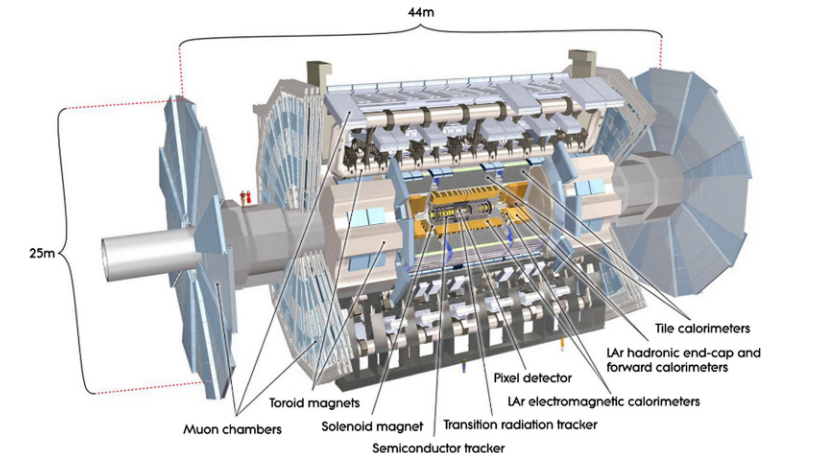
\includegraphics[scale=0.5]{chapter2/ATLAS.png}
\caption{Inner view of ATLAS detector,~figure taken from~\cite{Schott_2014}.}
\label{ATLAS_VIEW}
\end{figure} 

\begin{figure}[H]
\centering
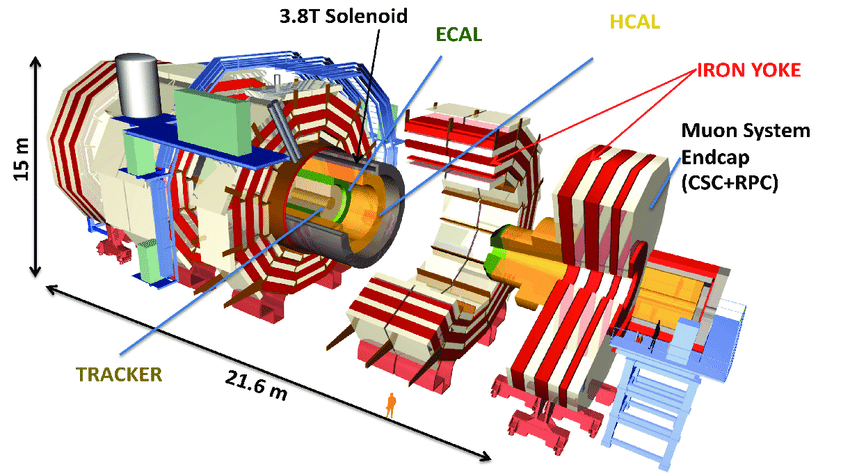
\includegraphics[scale=0.5]{chapter2/cms.png}
\caption{Schematic illustration of the CMS detector,~figure taken from~\cite{article11}.}
\label{cms1}
\end{figure}


\subsubsection{A Large Ion Collider Experiment~(ALICE)}
The ALICE~\cite{Collaboration_2008alice} is designed to study the properties of quark–gluon plasma, a rare state of matter. Quark-gluon plasma is the state of matter under very high temperature and densities in which quarks are free and not confined inside a hadron. 

\begin{figure}[H]
\centering
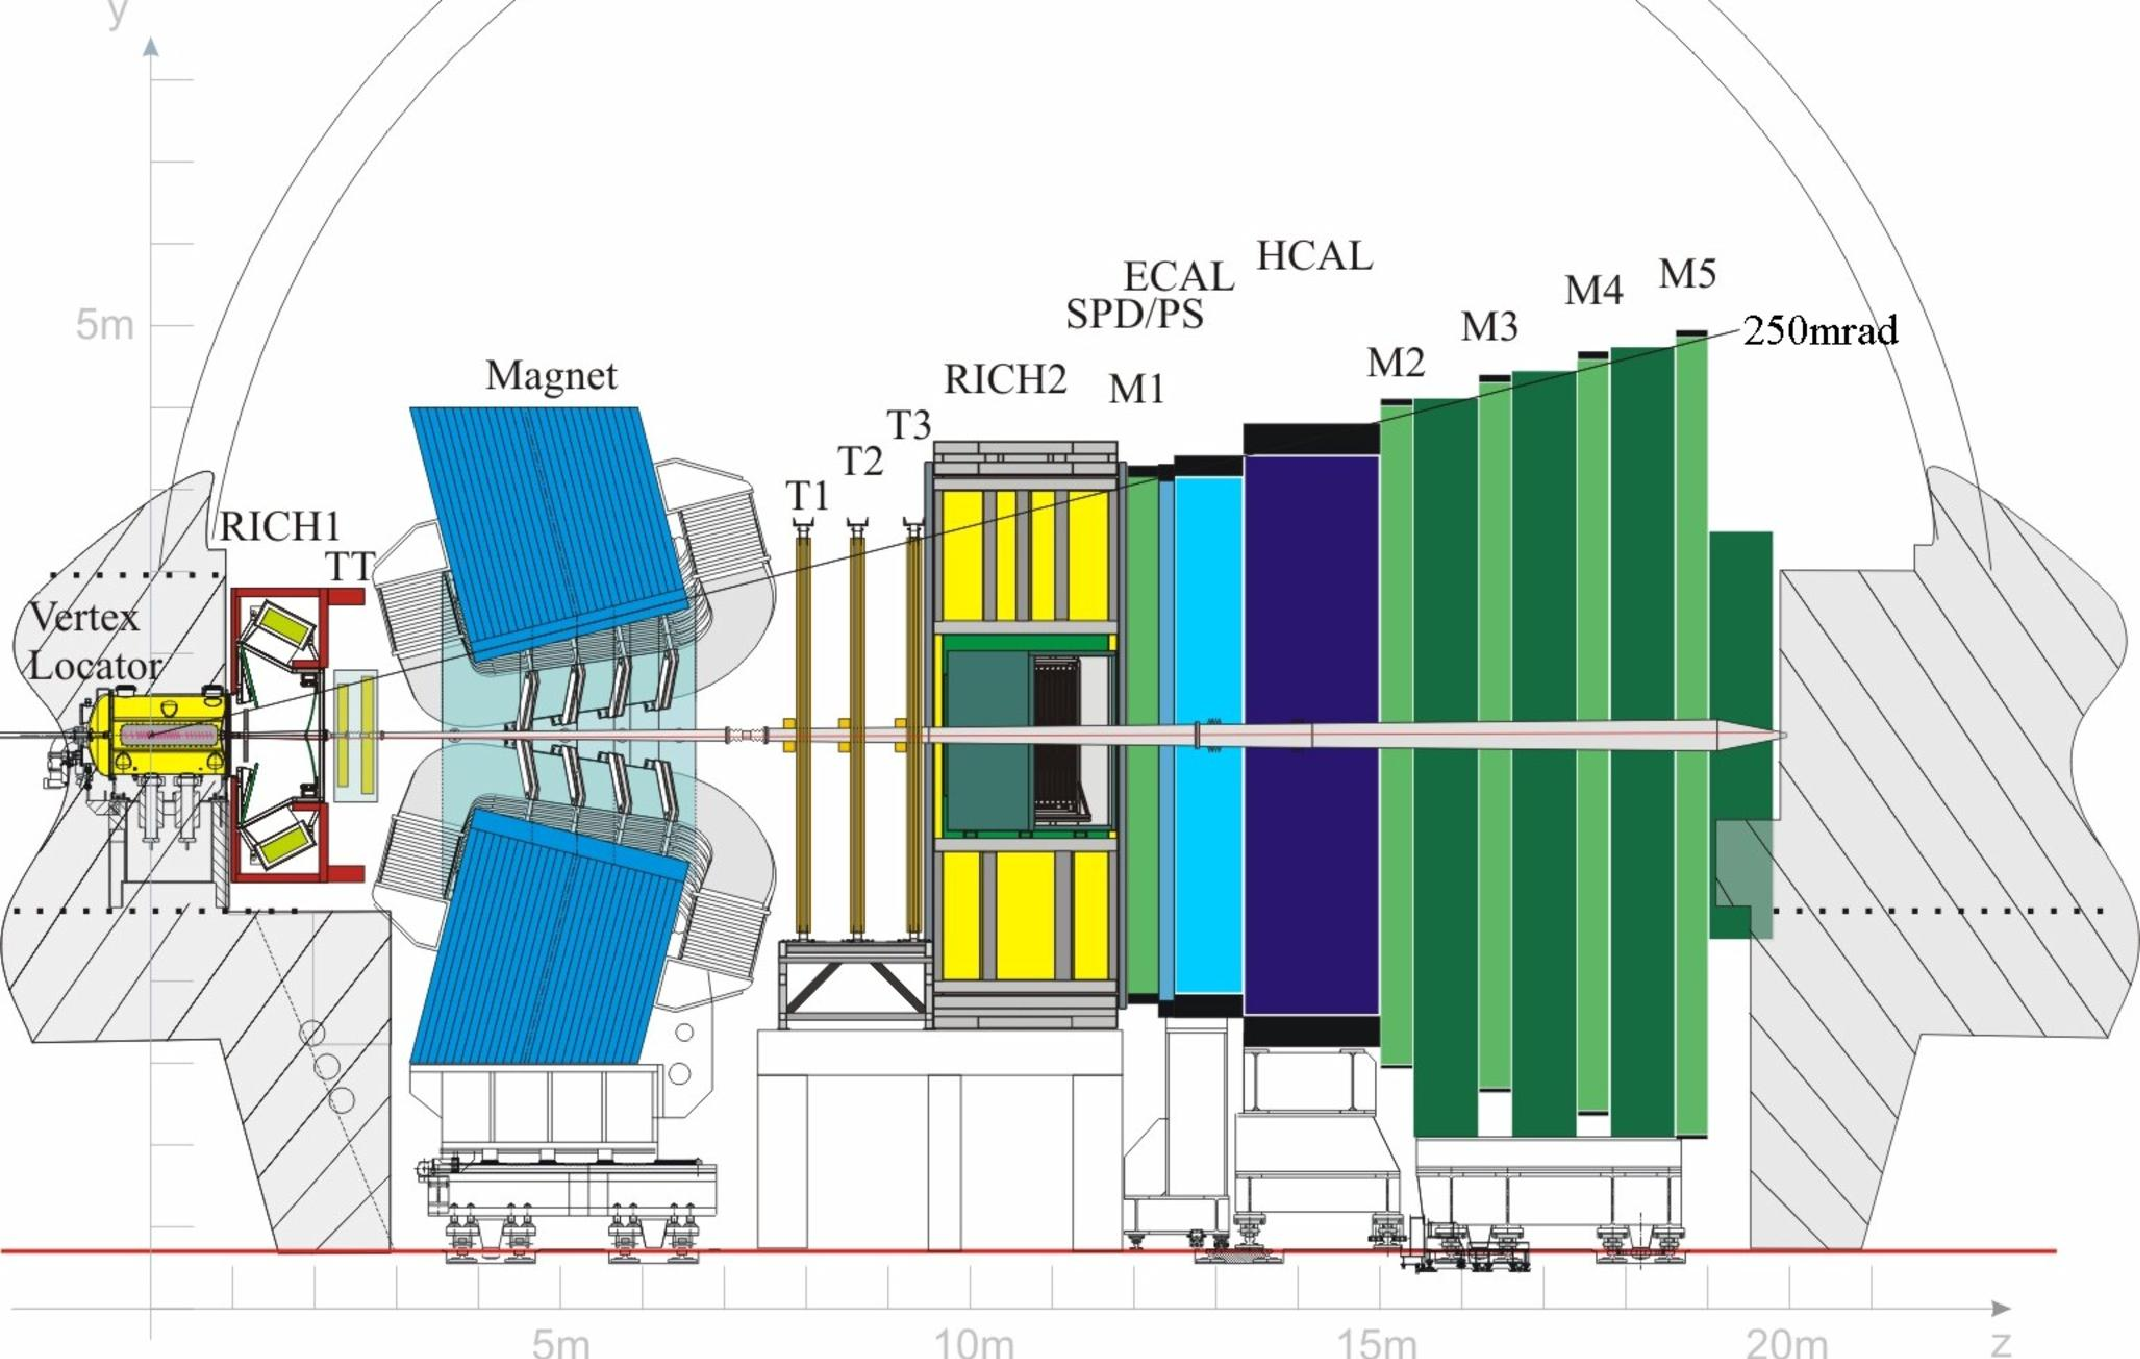
\includegraphics[scale=0.2]{chapter2/LHCb.png}
\caption{Inside view of the LHCb detector at LHC,~figure taken from~\cite{Mead:2780780}.}
\label{lhcb}
\end{figure}

\subsubsection{Large Hadron Collider Forward~(LHCf)}
The large hadron collider forward~(LHCf)~\cite{Collaboration_2008lhcf} is a small experiment that is designed to study different aspect of nuclear physics.

\subsubsection{TOTEM}
TOTEM~\cite{Collaboration_2008} is designed to measure the total cross section, elastic and diffractive scattering of the proton. TOTEM is able to detect particles that are produced very close to the beam pipe of LHC. The TOTEM is placed in a specially designed vacuum chambers called Roman pots. These Roman pots are connected to the beam pipes around LHC. There are total of 26 Roman pots in LHC which are located near CMS experiment as shown in Fig.~\ref{Totem}.

\begin{figure}[H]
\centering
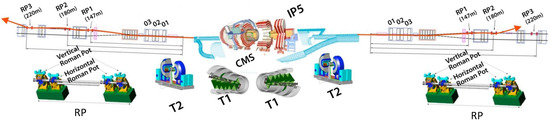
\includegraphics[scale=0.7]{chapter2/totem.jpg}
\caption{Sketch of the TOTEM and CMS experiments at the LHC~figure taken from~\cite{article}}
\label{Totem}
\end{figure}

\section{Parameters Of LHC}
\subsection{LHC Co-ordinate System}
The CMS and ATLAS detectors work using the right-handed cartesian system with center being the origin of the co-ordinates at the point where the interaction takes place. The $x-axis$ is directed towards the center of the hadron collider, the $y-axis$ is directed in the upward direction that is perpendicular to the ground whereas the third $z-axis$ is parallel to the proton beam, as shown in Fig.~\ref{co-ordinate lhc}. The polar angle, $\theta$, is the angle measured w.r.t the beam axis. The azimuthal angle, $\phi$, is the angle between the x-y planes. The distance $\Delta r$ between two particles is defined in the $\eta-\phi$ plane as
\begin{equation}
\Delta r = \sqrt{\Delta \eta^{2}+\Delta \phi^{2}}
\end{equation}
where $\Delta \eta=|\eta_{a}-\eta_{b}|$, $\Delta\phi=|\phi_{a}-\phi_{b}|$ and $\eta, \phi$ are polar and azimuthal angle of the particle tracks.
\begin{figure}[H]
\centering
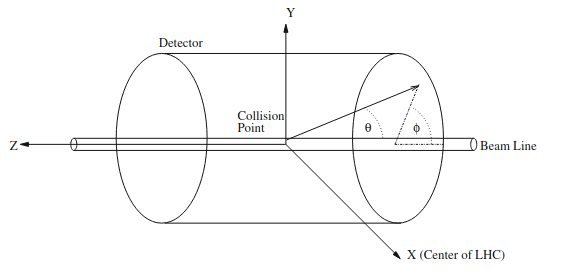
\includegraphics[scale=0.6]{chapter2/coordinate.png}
\caption{ATLAS and CMS coordinate system,~figure taken from~\cite{Schott_2014}}
\label{co-ordinate lhc}
\end{figure}
\subsection{Pseudo rapidity}
In hadron collider physics, a useful term defined as rapidity of the particle is given as
\begin{equation}
y=\frac{1}{2}ln\frac{E+p_{z}}{E-p_{z}} 
\end{equation}
where $p_{Z}$ is the momentum of particle along $z-axis$. The term pseudo rapidity '$\eta$' is derived from rapidity,~commonly measured in polar angle $\theta$ with respect to beam axis. Pseudo rapidity is defined by the equation $\eta=-\ln(\tan\frac{\theta}{2})$.
\begin{figure}[H]
\centering
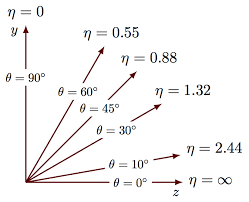
\includegraphics[scale=0.6]{chapter2/pseudorapidity.png}
\caption{Pseudo rapidity values in $1^{st}$ quadrant}
\end{figure}
where '$\theta$' is the angle between particle direction and beam direction.  The transverse momentum '$p_{T}$' is defined as the component of particle momentum in x-y plane. The transverse energy is defined as $E_{T} =
E sin\theta$.

The energy which is carried by non detectable particles is called missing energy, because these particles have no interaction through strong or electromagnetic forces, these particles are called neutrinos. In general, missing energy arises due to presence of non-detectable particles in the detector. The particle travelling in transverse direction to the beam axis have zero initial momentum, so if we have final momentum in $x$ or $y$ direction, it represents the missing transverse energy, because the total transverse momentum of initial state is zero, sum of final state particle’s transverse direction should also be zero. Missing transverse momentum~\cite{PortilloQuintero:2668716} can be defined by following equation,
\begin{equation}
\overrightarrow{E}_{T}^{missing}=-\Sigma_{i}\overrightarrow{p}_{T}^{i}
\end{equation}
Where, the index $i$ sums over all visible particles. The assumption that transverse energy and momentum are equal, holds only for particles that are massless.
The missing transverse momentum is defined as
\begin{equation}
\overrightarrow{p}_{T}^{missing}=-\Sigma_{i=1}^{N}\overrightarrow{p}_{T_{i}}
\end{equation}
In an event $N$ is the total number of final state particles. The $p_{T} $ and $p_{T}^{missing}$ are invariant under Lorentz boost along the beam direction which is $z-axis$. 
For particles of mass very smaller than their energy $(m<<E)$ the rapidity can be approximated by pseudo rapidity $\eta$.
\subsection{Luminosity}
Luminosity~\cite{Aberle:2749422} is a important parameter of the accelerator. To observe new phenomena in experimental high energy physics, we required high center of mass energy such as up to $14~TeV$, as well as large number of useful interactions. These useful interactions are used to reconstruct data for the analysis. In the study of rare events with very small cross section $\sigma$, luminosity becomes more important. The total number of interactions that an accelerator can produce is called its luminosity and it is the proportionality factor between event production rate $\frac{dR}{dt}$ and the cross section $\sigma$:
\begin{equation}\label{ins-lumi}
\frac{dR}{dt}=\mathcal{L}_{ins}.\sigma
\end{equation}
Luminosity can be defined simply by, ratio of the number of events produced~$(dN)$ in a certain time~$(dt)$ to cross section $\sigma$. 
\begin{equation}\label{ins-lumi}
\mathcal{L}_{ins}=\frac{dN}{\sigma dt}
\end{equation}
 
The unit of luminosity is $cm^{-2}s^{-1}$. The rate of collisions also relate to instantaneous luminosity $\mathcal{L}_{ins}$ as:
\begin{equation}\label{in_lumi}
N=\mathcal{L}_{ins}\times\sigma
\end{equation}
Where $\sigma$ is cross section of expected process. Equation~\ref{in_lumi} shows that the instantaneous luminosity cannot be kept stable during the data taking~\cite{Waqas:2779481}. $\mathcal{L}$ decreases due to loss of protons in bunches, which leads to decrease in collision rate. Therefore, another useful quantity in detector physics integrated luminosity~$\mathcal{L}_{int}$ is introduced by integrating the instantaneous luminosity over time, having units inverse barns denoted by $b^{-1}$ (per $cm^{2}$). It is used to measure how much data is recorded by LHC and CMS.\\
The data acquisition system  of detector is not always 100~$\%$ efficient due to which the amount of data recorded by a detector is usually smaller than the amount of data delivered, and not all the data is good enough for analysis purpose, as some of the subsystems may be in an error state that corrupt the data recorded or other unexpected behaviour of the LHC or CMS may have interrupted the data recording. The total amount of data used in an analysis can be much smaller than the total amount of data delivered. Fig.~\ref{CMS_lumi} shows the predicted increase in luminosity of CMS detector with center of mass energy.
\begin{figure}[H]
\centering
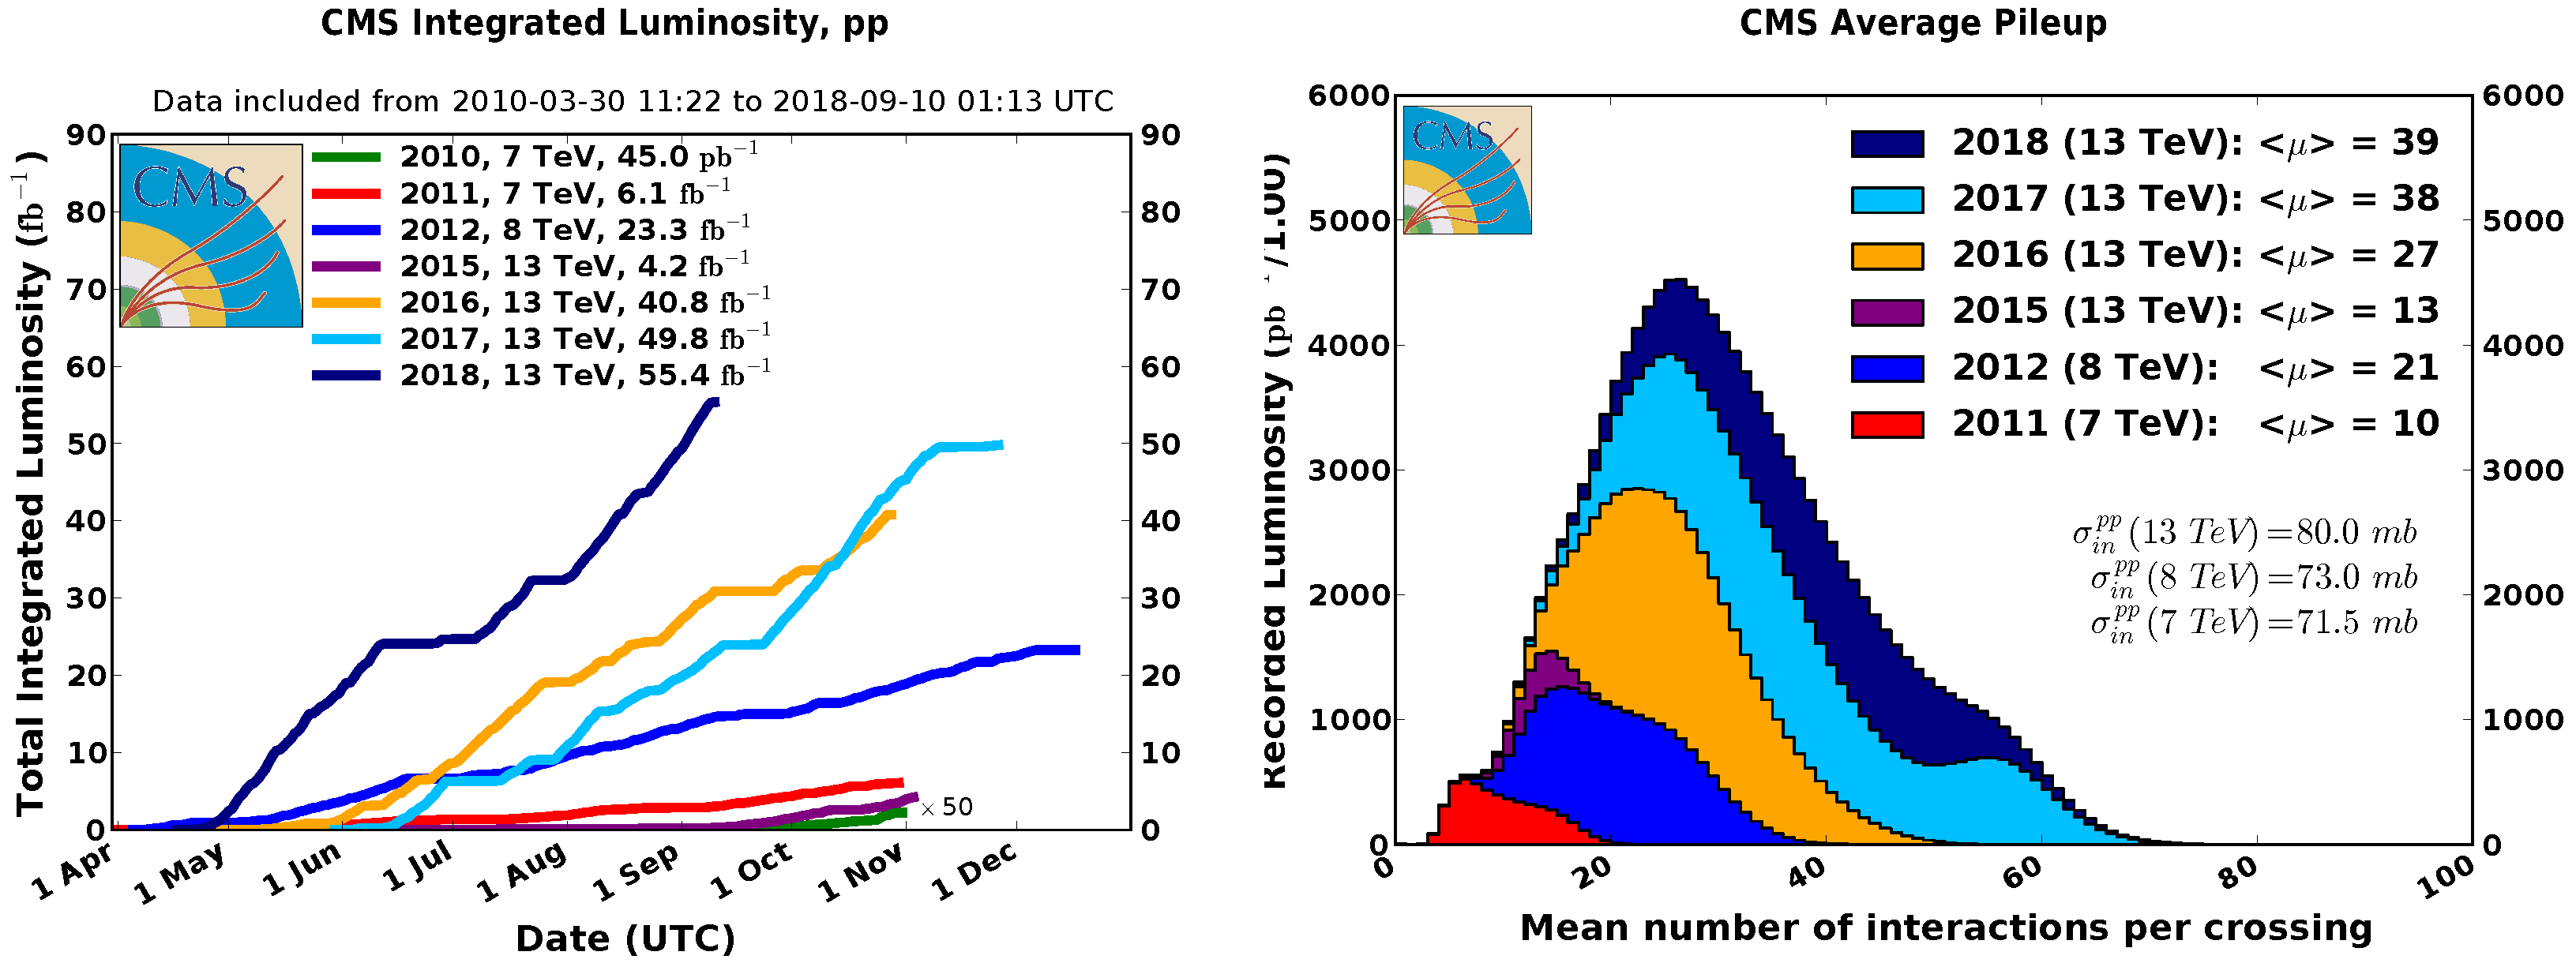
\includegraphics[scale=1]{chapter2/cms-lumi.png}
\caption{$\mathcal{L}_{int}$ delivered to CMS versus data taking period for pp collisions at different LHC energies. The distribution of $<\mu>$ versus luminosity recorded by CMS for the 2011~-~2012 and 2015~-~2018 data taking period~figure adopted from~\cite{Aberle:2749422}. }
\label{CMS_lumi}
\end{figure}
\subsection{Pile-up (PU)}
Another important parameter of the accelerator is pileup. During a bunch crossing multiple proton-proton interactions can occur which are referred to as pileup. These interactions are proportional to the event cross section times luminosity. There are two types of pileups:
\begin{itemize}
\item in-time PU comes from the collisions happening in the same bunch crossing.
\item out-of-time PU comes from the collisions from the previous bunch crossings whose signal has not yet been recorded by the detector.
\end{itemize}
In-time PU is calculated by the number of primary vertices ($N_{PV}$ ) while out-of-time PU is parametrized by the mean number of interactions per bunch crossing ($\mu$). In 2012 an average of 21 pileup interactions was observed at $8~TeV$. This increased in 2016 due to the higher luminosity and cross section at $13~TeV$, to about 27 interactions on average. 


\subsection{Beam Spot}
This spot is the brightest region where the two beams travelling in opposite direction are brought into collision. It is an important and an essential parameter for the computation of different parameters which are used in further data analysis. It is very necessary to measure beam spot very accurately and precisely, especially the beam spot width, the value of beam spot width is further used by computation procedure of different observables. It is also a reference point for studying the track performance.

\section{CMS Detector}
The Compact Muon Solenoid (CMS)~\cite{Collaboration_2008cms}, as the name represents is compact due to small size when compared to ATLAS detector, muon is a fundamental particle detected by CMS, and solenoid for the large superconducting magnet. The side view of CMS detector is shown in Fig.~\ref{CMS_sideview}. The scientific goals of CMS experiment are same as for the ATLAS. After the discovery of Higgs boson, the study of Higgs boson properties in detail and search for the physics beyond the Standard Model are the main goals of CMS experiment. CMS has a different technical solution, especially its magnetic system design.\\
The CMS detector built $100m$ underground in France countryside, near the village of Cessy. One of the main goals to built CMS experiment was the search of Higgs boson that is responsible of electroweak symmetry breaking. This goal was achieved in $2012$ by the discovery of scaler boson named "SM Higgs Boson"~\cite{Chatrchyan_2012}. CMS experiment covers many aspects of proton-proton collisions at very high center of mass energy i.e.~($14~TeV$) of the LHC. 
Some of the main characteristics of CMS are as follows:
\begin{itemize}
\item CMS provides a better muon identification and momentum measurement over wide range of angle.
\item CMS tracking system provides good identification of the charged particles.
\item A wide geometric coverage, better electromagnetic energy resolution.
\end{itemize}
\subsection{Structure of CMS}
The CMS detector has a long cylinder of length $21.6~m$ with a diameter of $15~m$ and weight $12500~tons$. It is designed to operate at a center-of-mass energy of $14~TeV$ and a luminosity of $10^{34}~cm^{-2}s^{-1}$. The CMS uses superconducting solenoid magnet that surrounds all the inner detectors. CMS is equipped with different types of silicon tracker,~i.e., silicon pixel and strip tracker, lead-tungstate~$(PbWO_4)$ Electromagnetic Calorimeter and a brass scintillator sampling Hadronic Calorimeter. An iron yoke which holds both superconducting solenoid and muon detector.\\ 
CMS has also right handed coordinate system, with the origin at the interaction point of beam inside the detector. CMS has cylindrical symmetry, it is convenient to use cylindrical co-ordinates $(r,\theta,\phi)$ shown in figure~\ref{cms-polar}.\\
The CMS structure can be summarized as below:
\begin{itemize}
\item The interactions between bunches of particles take place at the core of the apparatus with a maximum instantaneous luminosity of $21~nb^{-1}s^{-1}$ achieved in LHC RUN 2.
\item The inner part of detector is silicon tracker which extend from interaction point to $|r|<1.2m$, covering $|\eta|$ range $<2.5$.
\item The Electromagnetic calorimeter~(ECAL) extends over $1.2m < r < 1.8m$ and covers pseudo-rapidity range $|\eta|<1.3$.
\item The Hadronic Calorimeter~(HCAL) covers $1.8~m < r <2.9~m$ by covering $|\eta|<5$.
\item The superconducting solenoid magnet provides a magnetic field of $4~T$ along the beam direction, which bends the charged particles trajectories in order to measure their momentum. The solenoid surrounds all the inner detectors and extends from $2.9~m < r < 3.8~m$ over $|\eta|<1.5$. 
\item The muon system is the outer most part of the CMS detector. It is extended from $4~m < r < 7.4~m$ and covers $|\eta|<2.4$.
\end{itemize}
\begin{figure}[H]
\centering
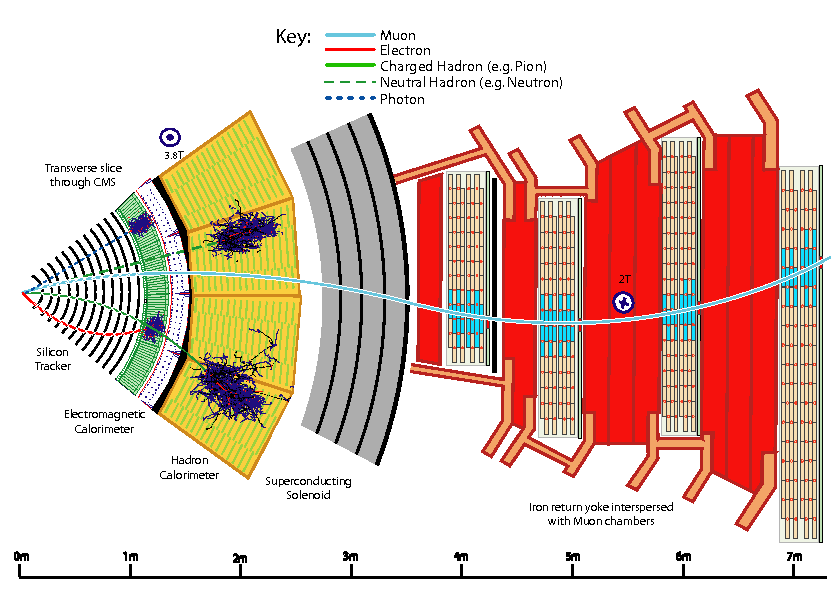
\includegraphics[scale=0.5]{chapter2/CMS_cutview.png}
\caption{Cut view of CMS detector, the distance of different components from center is illustrated in figure taken from~\cite{Davis:2204863}}
\label{CMS_sideview}
\end{figure}

\begin{figure}[H]
\centering
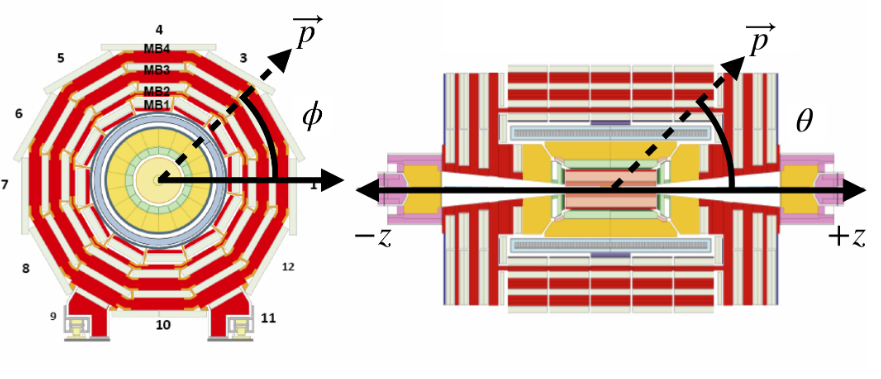
\includegraphics[scale=0.48]{chapter2/cms-coordinate.png}
\caption{Polar coordinates used by CMS. Figure taken from reference~\cite{Collaboration_2010}.}
\label{cms-polar}
\end{figure}


\subsection{CMS Tracker}
The tracker is located very close to the interaction point as shown in Fig.~\ref{CMS_schematic} hence it receives the largest number of particles produced. The tracker is designed to measure highest resolution of charged particles trajectories with transverse momentum up to $1~GeV$ in a range $|\eta|=2.5$. At LHC 
design luminosity of about $10^{34}~cm^{-2}s^{-1}$, the tracker records roughly 100 tracks per bunch crossing,~i.e., for every $25~ns$. So it is necessary to choose the construction material carefully to resist high radiation and particle flux.
\begin{figure}
\centering
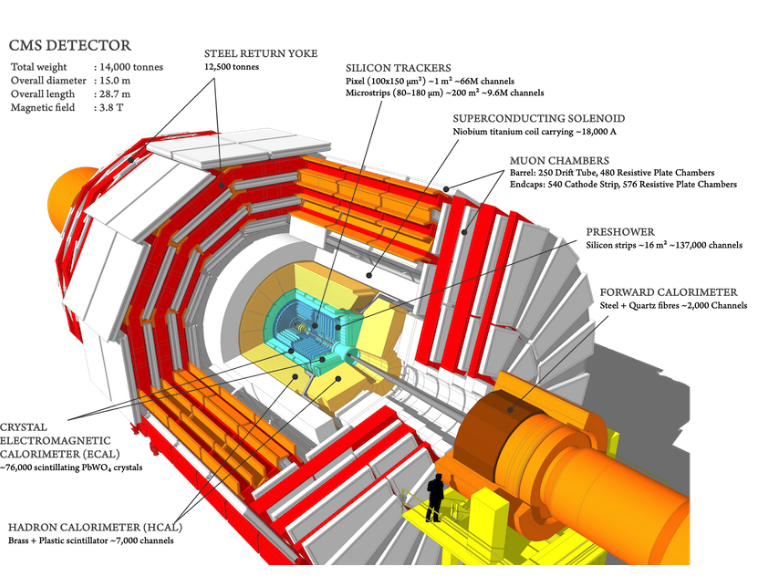
\includegraphics[scale=0.5]{chapter2/cms-schematic.png}
\caption{Schematic view of CMS detector. Figure taken from~\cite{Layter:343814}.}
\label{CMS_schematic}
\end{figure}

\subsection{Electromagnetic Calorimeter~(ECAL)}
The ECAL~\cite{CERN-LHCC-97-033} sits in between the tracker and Hadron Calorimeter~(HCAL). It is designed to detect and measure the energy of photons, electrons and positrons with great precision. There are three partitions in ECAL: Barrel, End caps and Pre shower. The ECAL barrel~(EB) has $61200$ $PbWO_{4}$ crystals, in a cylindrical shape design that begins at a radius of 1.29~m  and covers the range $|\eta| < 1.479$. The barrel has a number of module and super module. The barrel region is complemented by $7324$ crystals that are mounted on two end caps located at 314~cm from the vertex and cover the range $1.47 < |\eta| < 3.0$.\\
The pre shower detector is placed in front of the end cap crystal and covers a range of $1.653 < |\eta| < 2.6$. It discriminates the electromagnetic shower formed by the photons, coming from the neutral pion decay. It also helps to identify the position of electrons and photons. The layout of ECAL can be seen in Fig.~\ref{ecal1}.

\subsection{Hadron Calorimeter~(HCAL)}
The Hadron Calorimeter~\cite{collaboration_2011} is designed for the study of many processes, which include energy and direction of hadronic jets, reconstruction of the hadron decays and missing transverse energy in the events. There are four modules of HCAL, the hadron barrel~(HB), hadron calorimeter end caps~(HE), the outer calorimeter~(HO), and the forward calorimeter~(HF).\\
The hadron barrel~(HB) shown in Fig.~\ref{hcal1} sits in between ECAL and superconducting magnetic coil at a distance $1.77~m < r < 2.95~m$. The hadron calorimeter end caps~(HE) cover the solid angle between $ 1.3 < |\eta| < 3$. The hadron barrel~(HB) calorimeter measures $860~cm$ in length with inner and outer radius of $177~cm$ and $295~cm$ respectively. HB is divided into two half-barrel HB+ and HB-. The end caps of HE cover range $1.3 < \eta < 3.0$. The HB+ and HB- have thirty six identical wedges. Each wedge is constructed from flat steel and brass plate and is aligned parallel to beam axis. The HE is also radially divided into 14 rings. The HO of HCAL is made with plastic scintillator in several layers and the most outer part of HCAL is HO which is $11.2~m$ away from the  collision point. 
\begin{figure}[H]
\centering
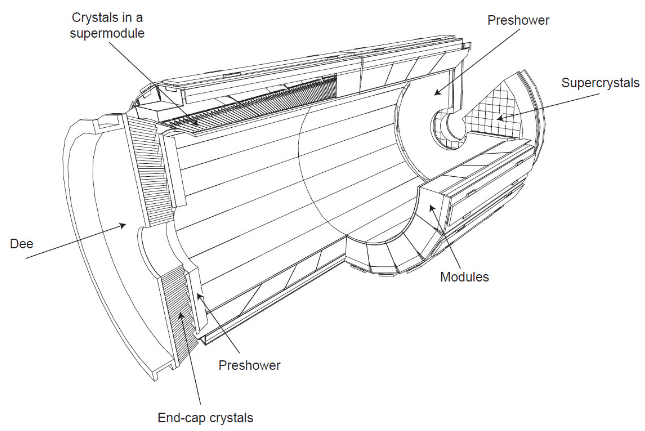
\includegraphics[scale=0.5]{chapter2/Ecal1.png}
\caption{CMS ECAL layout,~figure taken from~\cite{Collaboration_2008cms}.}
\label{ecal1}
\end{figure}
\begin{figure}[H]
\centering
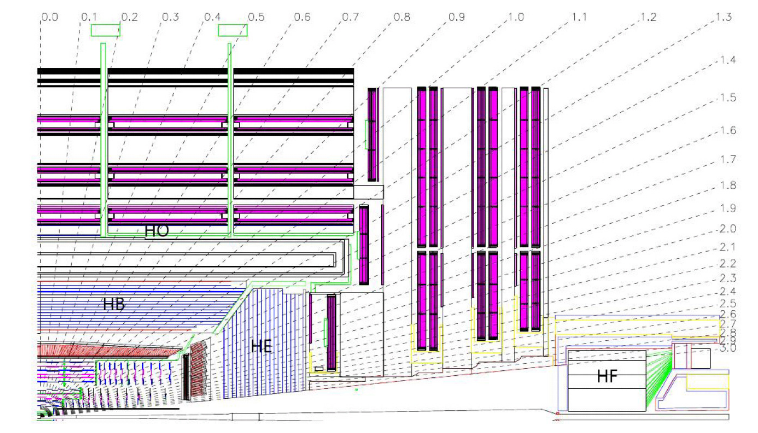
\includegraphics[scale=0.5]{chapter2/Hcal1.png}
\caption{Layout of CMS HCAL,~figure taken from~\cite{Collaboration_2008cms}.}
\label{hcal1}
\end{figure}

\subsection{Magnetic System of CMS}
The distinct feature of CMS is its superconducting magnet~\cite{Klyukhin:2773274} designed to provide magnetic field of $4~T$ in a region of length $12.5~m$ and $6~m$ in width, one of the biggest solenoid ever made.\\
In CMS detector we need high magnetic field to bend particle trajectories which is obtained by combination of different magnets made by NbTi cables. The energy stored at an operating temperature of $4.6~K$ and at full current is $\approx$ ~$2.6~GJ$. The magnetic flux of these coils is returned through an iron yoke weighing $10,000~tons$. It is shown in Fig.~\ref{CMS_magnet}. 

\begin{figure}[H]
\centering
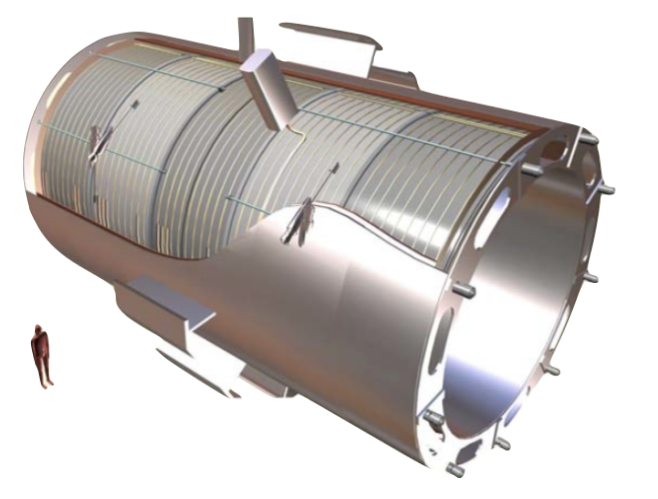
\includegraphics[scale=0.5]{chapter2/magnetic-cms.png}
\caption{View of CMS superconducting solenoid. Figure adopted from~\cite{Collaboration_2008cms}.}
\label{CMS_magnet}
\end{figure} 

\subsection{CMS Muon System}
The CMS muon system~\cite{Sirunyan_2018} is specially designed to detect muons with high transverse momentum. Its main function is to identify muon, measurement of its momentum and triggering.\\
The muon system of CMS is divided into three independent subsystems, which consist of three gaseous particle detectors, the drift tube system, cathode strip chambers and the resistive plate chambers.\\
\subsubsection{Drift Tube Chamber}
The barrel region of CMS muon system is instrumented with drift tube~(DT) chambers covering the pseudo-rapidity range up to $|\eta|~=~1.2$. The DT chambers arranged into five iron wheels, each wheel have four concentric ring called stations. The function of these stations is to measure the muons coordinates in the transverse plane as well as its $z$ direction.\\
The detector of this chamber is a drift tube of rectangular shape of size $ 13\times42~mm^{2}$ and having length $2-4~m$. The whole volume is filled with gas mixture of $85\%$ argon and $15\%$ carbon dioxide.\\
\subsubsection{Cathode Strip Chamber}
The cathode strip chamber is installed at the end cap of CMS muon system. This chamber is designed especially to identify muons in the region $0.9 < |\eta| <  2.4$. The chamber is divided into four stations for each end cap, perpendicular to the beam pipe and separated by the flux return plate as can be seen in Fig.~\ref{csc1}.\\ 
\begin{figure}[H]
\centering
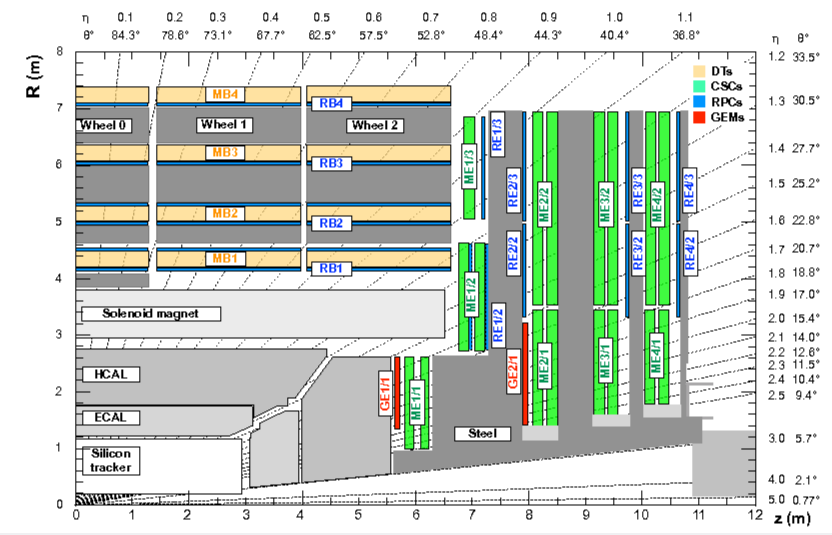
\includegraphics[scale=0.5]{chapter2/csc1.png}
\caption{CMS muon detector system. Figure adopted from~\cite{Sirunyan_2018}.}
\label{csc1}

\end{figure}
The cathode strip chamber is filled with $40\%$ argon and $50\%$ carbon dioxide as active gas and remaining $10\%$ with carbon tetrafluoride. This chamber is arranged in four disks called stations, each of which has two rings divided into eighteen or thirty six CSCs. These stations are equipped with sensitive wires which provide muon recognition.

\subsubsection{Resistive Plate Chamber}
The resistive plate chambers~(RPC) are installed at both barrel and end cap regions. They are also gaseous detector. The RPCs are made of four Bakelite planes coated with graphite which act as the electrode and two gas gaps of $2mm$.\\

\subsection{CMS Trigger System}
LHC provides proton-proton and heavy ions collisions at a very high rate as shown in Fig.~\ref{recoreder_lumi}. High particle density in each bunch corresponds to an event rate of 40 MHz with 20 head-on collisions per event, thus interaction rate exceeds 1~GHz. Such a high data stream cannot be handled with current available technology. Therefore, CMS experiment uses a dedicated trigger system. The trigger system selects possible events of interest among all the simultaneous events occurring.\\
The trigger system~\cite{Khachatryan_2017} is divided into two main stages:\\
\begin{enumerate}
\item Level-1 trigger~(L1) system consists mainly of programmable electronic components.
\item High Level Trigger~(HLT) system is fully software based.
\end{enumerate} 
The L1 trigger preselects events of interest in order to be further analysed by the HLT. L1 trigger is responsible for the identification of different leptons, quark jets and missing transverse energy. It consists of three main subsystems:
\begin{itemize}
\item Calorimeter Trigger
\item Muon Trigger
\item Global Trigger
\end{itemize}  

\begin{figure}[H]
\centering
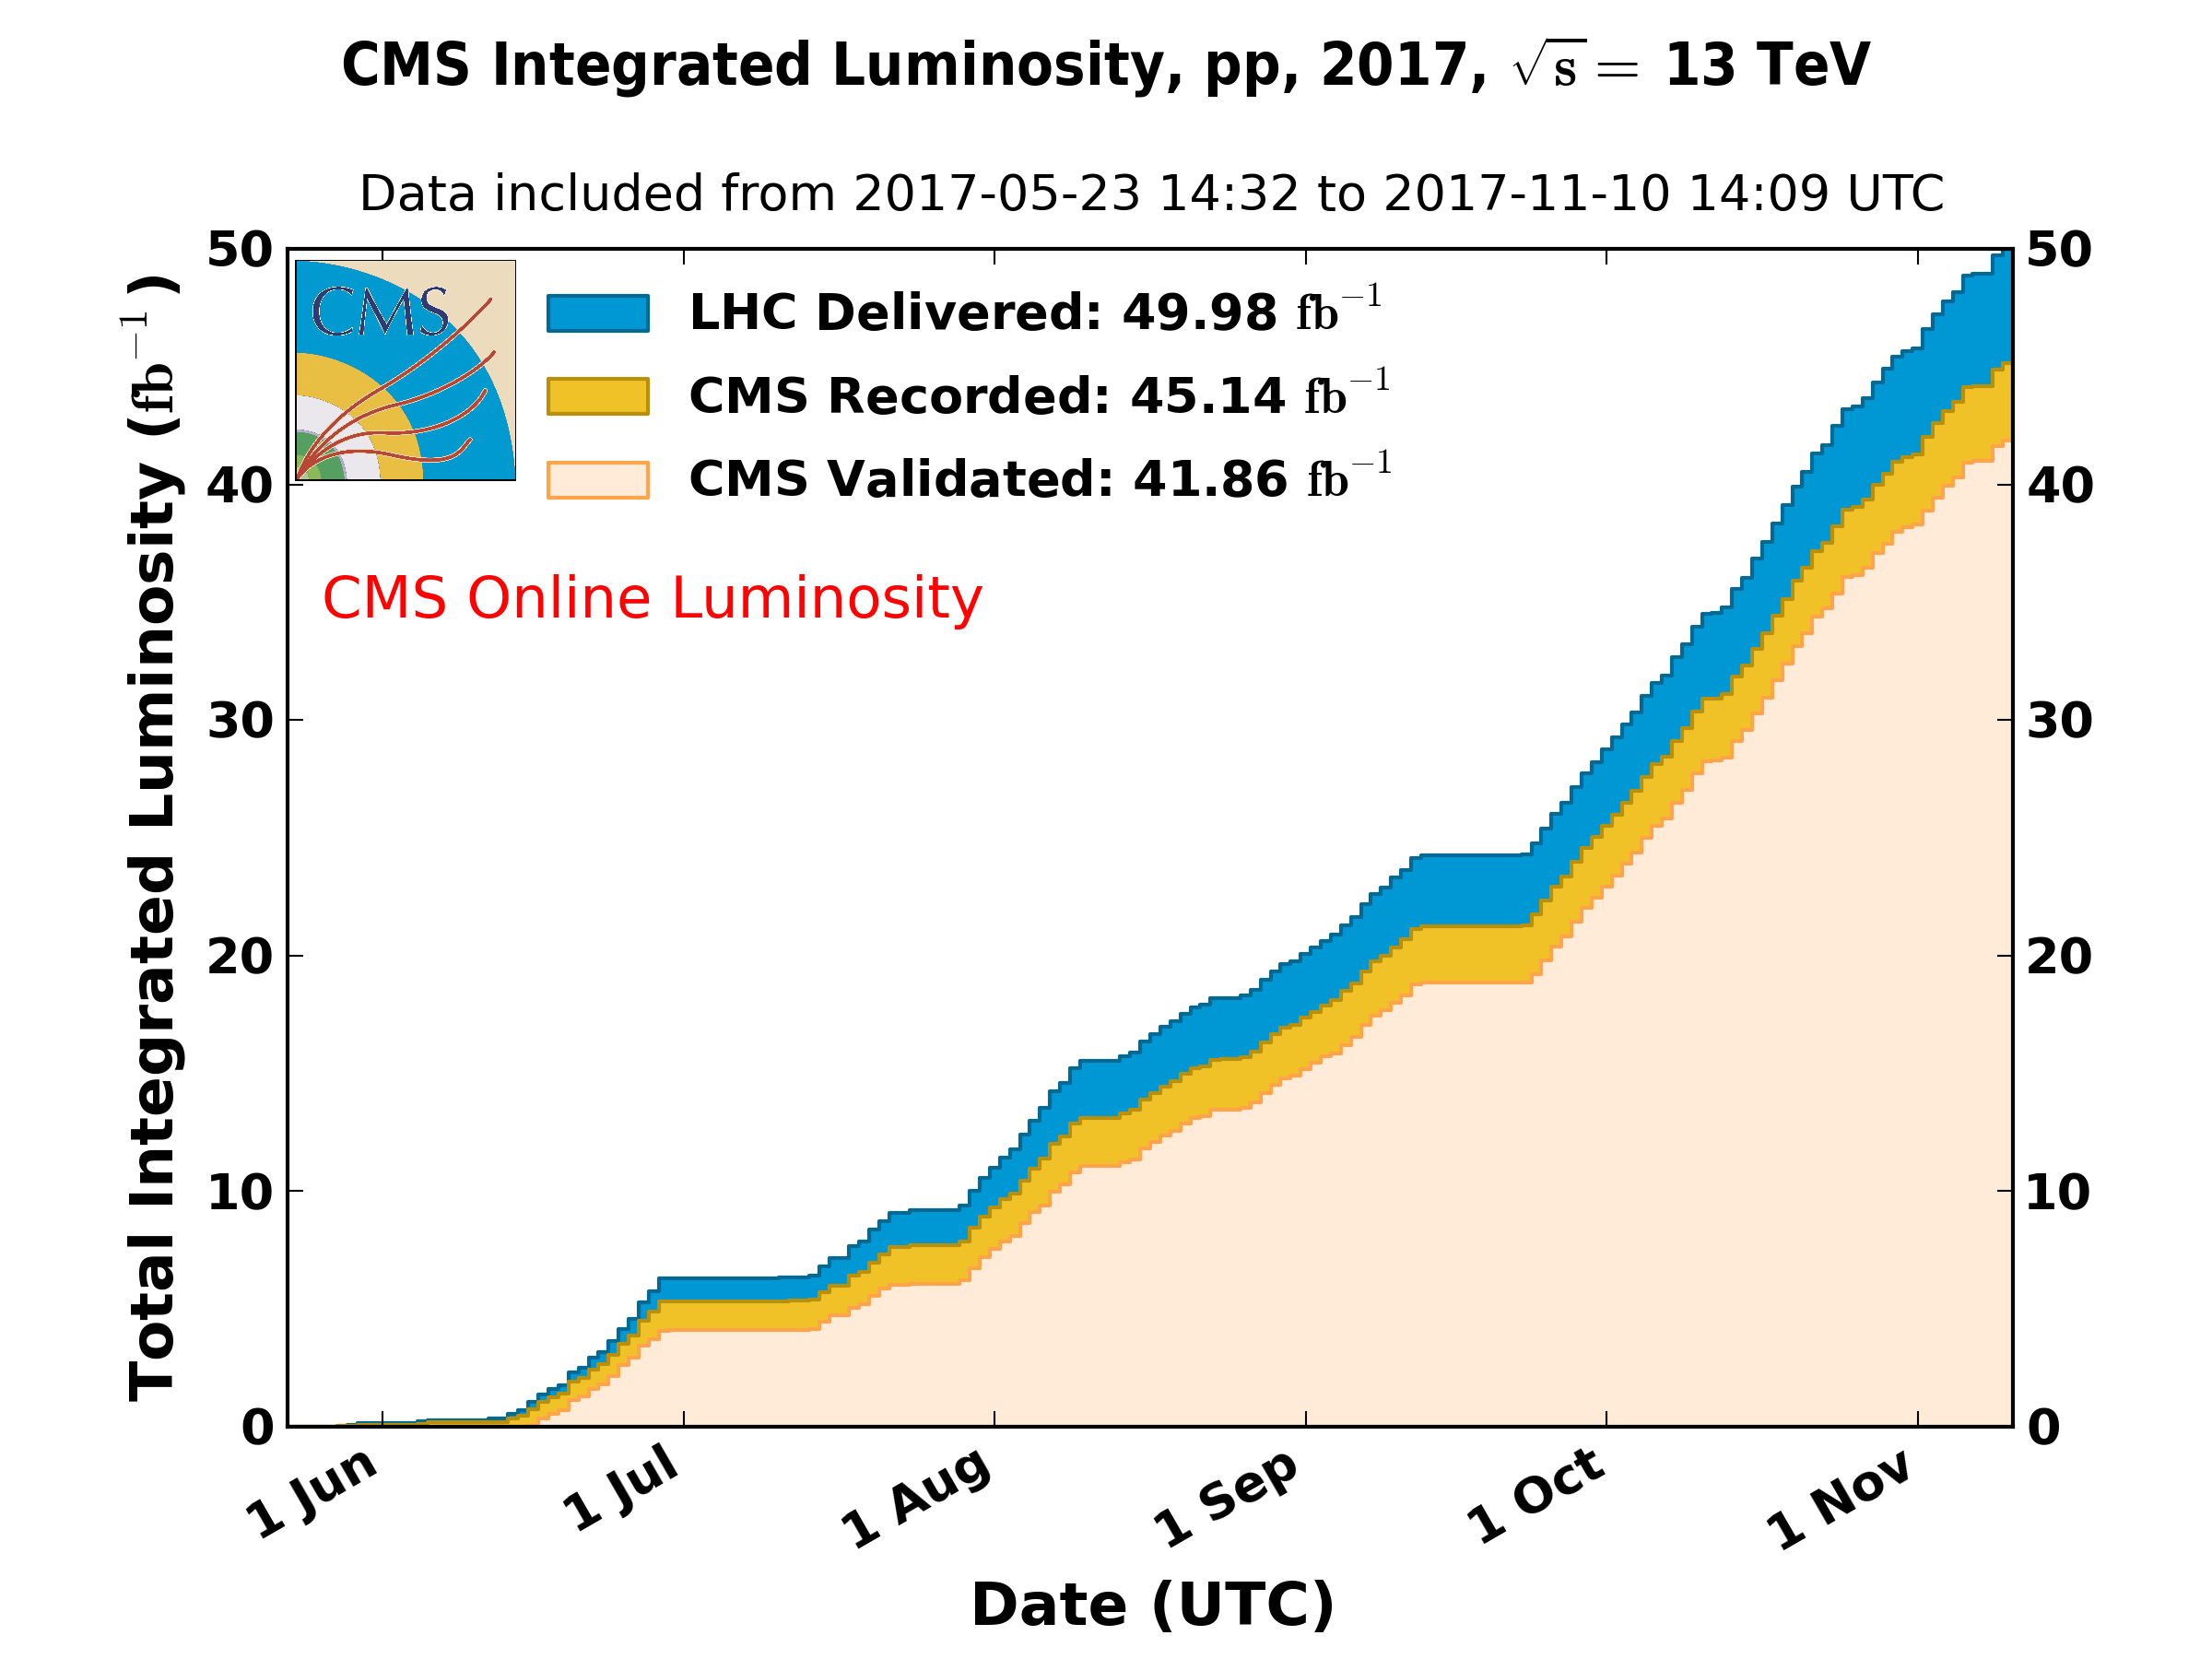
\includegraphics[scale=0.5]{chapter2/cms luminosity.png}
\caption{CMS recorded luminosity at $13~TeV$.}
\label{recoreder_lumi}
\end{figure} 


The event selection at the \textbf{HLT}~\cite{Cittolin:578006} is similar to that used in the offline processing. HLT reconstructs the leptons, jets and applys the identification criteria in order to select only those events which are of possible interest for data analysis. A view of the CMS L1 trigger is shown in Fig.~\ref{cms-trigger}.

\begin{figure}[H]
\centering
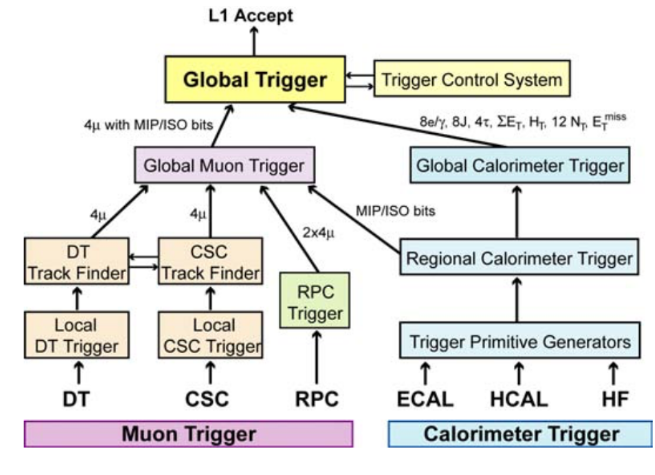
\includegraphics[scale=0.5]{chapter2/cms-trigger.png}
\caption{The L1 trigger system of CMS,~figure taken from~\cite{Collaboration_2008cms}.}
\label{cms-trigger}
\end{figure} 





\chapter{Theory of Single Vector Bosons}
The vector boson production cross section measurement during hadron collision, provides a deep understanding of quantum chromodynamics (QCD) and electroweak (EW) processes. The production of $W$ and $Z$ bosons are best examples of hard scattering processes at Large Hadron Collider. Theoretical predictions in perturbative chromodynamics are available at next-to-next-to-leading order~(NNLO)~\cite{PhysRevD.51.44, VANNEERVEN199211}.
 
The cross sections of $Z$ and $W$ boson and their ratios are experimentally measured by the ATLAS and CMS detector at the Large Hadron Collider~(LHC) in  proton-proton collisions at various center of mass energies. This thesis presents theoretically predicted cross section of the $W$ and $Z$ boson production cross section in a proton proton collision at $\sqrt{s}=13~TeV$~\cite{2016601}.

\section{Significance of $W$ and $Z$ Boson Production Cross Section}
The $W$ and $Z$ electroweak bosons were discovered at UA1~\cite{UA1:1983crd} and UA2~\cite{UA2:1983mlz}, and their detailed measurements have been done at electron-positron and hadron Collider. LEP~(Linear electron-positron) performed many accurate measurements for the study of these vector bosons, with a precision of $1~\%$~\cite{guageboson}. At Large hadron colliders, single vector boson production has been performed  at various center of mass~(C.O.M) energies i.e. $\sqrt{0.63}~TeV$ at the CERN S$p\overline{p}$S~(Super Proton Anti proton Synchrotron) by UA1 and UA2, at $\sqrt{1.8}~TeV$ at the Tevatron by CDF~(Collider Detector at Fermi lab)~\cite{PhysRevLett.62.1005} and  at $\sqrt{1.96}~TeV$ by D0~(DZero)~\cite{PhysRevLett.100.102002}. There are large number of $W$ and $Z$ events produced in Large Hadron Collider, which help us to measure production cross section of these bosons easily, roughly around 140,000 events for $Z\rightarrow ee$ and 500,000 $W\rightarrow e\nu$ events are recorded with $2.2~fb^{-1}$ of data. Measurements of production cross section of vector bosons at the $Sp\overline{p}S$ and the Tevatron are very important, as these measurements provide data for the development of leading-order~(LO) and next-to-leading order~(NLO) theoretical predictions and results of these measurements are also used for comparison with data at the LHC. LHC provides measurement of $W$ and $Z$ boson at higher energy regimes, so we can improve our  theory of perturbative Quantum Chromodynamics~(QCD). The results at higher energy regime also provide more constraints on the parton distribution function~(PDF) along with improvement in electroweak precision measurements, i.e mass of charged vector boson $W$ and $sin^{2}\theta$. These new measurements of vector bosons at LHC provide deep insight for the study of new physics including measurement of Higgs boson parameters, top quark physics and physics beyond the standard model.\\
Increase in energy at LHC benefits for the predictions of perturbative QCD, Fig.~\ref{fig1} illustrates these benefits.  We can reach further lower Bjorken $x-$value for any process, e.g the production of $Z$ vector boson shown here. With these new energy regimes we can reach more low $x$ region as compared to SPS and Tevatron experiments. This may improve statistical and systematic uncertainties. Millions of vector boson events have been detected at CMS and ATLAS experiments. These new detectors can measure electrons up to to $|\eta|<4.9$ and jets to $|\eta|<4.4$ and a large fraction of low-$x$ events can be reconstructed by the LHC detectors.   


\section{Theory of Single Vector Boson Production}
The theoretical predictions used for comparison of $W$ and $Z$ boson production cross section have been improved. The theoretical predictions in perturbative QCD theory are available up to next-to-next-to-leading order~(NNLO). Theoretical predictions at next-to-leading order(NLO) for the production cross section of vector boson in association with jets exist for five partons in the final state. The uncertainties in  theoretical prediction  are comparable with experimental uncertainties. We will discuss about different types of theoretical uncertainties in last section of this chapter.
\begin{figure}{h!}
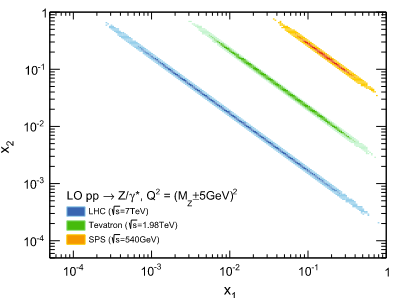
\includegraphics[scale=1]{chapter3/bjorkenx.png}
\caption{Correlation of LHC, Tevatron and SPS hadron Collider between the $x$ values of the interaction of two partons~\cite{Schott_2014}}.
\label{fig1}
\end{figure}
 
\subsection{Cross Section Calculation}
There are two energy regimes for the calculation of production cross section in proton-proton collisions at Large Hadron Collision(LHC)
\begin{itemize}
\item High-energy regime also called short distance regime
\item Low-energy regime also called long distance regime
\end{itemize}
In perturbative QCD there are two terms in the factorization theorem: one is $\hat{\sigma}_{q\overline{q}}\rightarrow n$ at short-distances for the parton-parton interaction and other is for large distances and explain the internal structure of proton. In case of very large momentum transfer $q$ in the interaction of parton, the interactions can be evaluated with perturbative QCD theory. The long-distance term or for low momentum transfer $q$, where perturbative QCD theory can not be applied, parton density function~(PDFs) describes the proton structure. These PDFs Functions can be written as $f_{\frac{a}{A}}(x,Q^{2})$ for the parton $a$ in the proton $A$, in which $x=\frac{p_{a}}{p_{A}}$ is shared momentum fraction for parton $a$ from proton's momentum and $Q^{2}$ is the energy scale of the scattering process.\\
The long-distance physics or physics at low momentum transfer and short distance physics or physics at high momentum transfer in parton-parton interaction, is separated by a scale called factorization scale $\mu_{F}=Q$~\cite{Mukhi:2019yrf}.
The cross section in the interaction of proton-proton is expressed by  
\begin{equation}
\sigma_{p_{A}p_{B}\rightarrow n}=\Sigma_{q}\int dx_{a}dx_{b}f_{\frac{a}{A}}(x_{a},Q^{2})\times f_{\frac{b}{B}}(x_{b},Q^{2})\hat{\sigma}_{ab\rightarrow n}
\end{equation}   
\begin{figure}[h!]
\centering
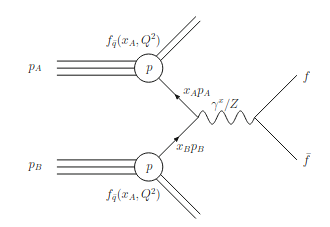
\includegraphics[scale=0.7]{chapter3/pdf.png}
\caption{Schematic of proton-proton collision at LHC.}
\label{p-p-collision}
\end{figure}
as shown in Figure~\ref{p-p-collision}. $f_{\frac{a}{A}}$ denotes the PDF of parton $a$ and $f_{\frac{b}{B}}$ is for parton $b$ in protons $A$ and $B$ respectively. All quark flavours are included in the sum and integration is performed over momentum fraction of parton $a$, $x_{a}$ and momentum fraction of parton $b$, $x_{b}$.\\
If we include the QCD corrections, then parton-parton cross section in term of $\alpha_{s}$ is,
\begin{equation}\label{qcd-correct}
\sigma_{p_{A}p_{B}\rightarrow n}=\Sigma_{q}\int dx_{a}dx_{b}f_{\frac{a}{A}}(x_{a},Q^{2})f_{\frac{b}{B}}(x_{b},Q^{2})\times[\hat{\sigma}_{0}+\alpha_{s}(\mu_{R}^{2})\hat{\sigma}_{1}+....]_{ab\rightarrow n}
\end{equation}
In Equation~\ref{qcd-correct},~ $\sigma_{1}$ is the correction in parton-parton cross section of order one, and $\sigma_{0}$ is the base-level parton-parton cross section. Therefore reference scale for the running strong coupling constant $\alpha_{s}(\mu_{R}^{2})$ is set by $\mu_{R}$~(re-normalisation scale). The re-normalisation scale~\cite{Mukhi:2019yrf} is set to eliminate the ultraviolet divergences in finite order cross section calculations.

\subsection{Parton Distribution Functions}

The quantum numbers of a hadron are determined by valance quarks. For example proton has two up quarks~($u_{v}$) and one down quark~($d_{v}$) and neutron has one up quark~($u_{v}$) and two down quarks~($d_{v}$). Along with these valance quarks, there are many quarks and anti quarks inside hadrons due to presence of gluons.
Deep Inelastic Scattering~(DIS)~experiments are best to probe the internal structure of nucleons, in which lepton acts as a probe by transferring four momentum $|q|$ to the nucleon in the collision. Electron-proton DIS experiment at SLAC in 1966 was the first evidence for the parton structure inside nucleons.\\
The resolving power of probe in DIS is~$\approx~\frac{\hbar}{|q|}$, and the level of structure that can be revealed is increased with $|q|$~i.e. we can get a resolution of $0.002~fm$ at $|q|=~100~GeV$, which is enough to probe the internal structure of proton.\\
The momentum distribution function of parton within nucleons is simply called Parton Distribution Function~(PDF). The PDF gives the probability~(normalised to the number of partons)~of finding the parton with momentum fraction $x$ at an energy scale $Q^{2}=-q^{2}$. DIS experiments show that at low $Q^{2}$ the three valance quarks are more and more dominant. For the high $Q^{2}$ values there will be many quark-antiquark pairs with low momentum fraction $x$. The result of DIS experiments show that, $\approx50\%$ of nucleon's momentum is carried by quarks and antiquarks and remaining is carried by gluons, momentum fraction carried by gluons is increased with $Q^{2}$. 
QCD predicts how parton distribution changes with $Q^{2}$ energy scale and these predictions are governed by the QCD evolution equation DGLAP in perturbative QCD domain, that is where the value of $\alpha_{s}(Q^{2})$ is much smaller than one. There are different levels of approximations for DGLAP equation, relative to the power of $\alpha_{s}(Q^{2})$ in the perturbative domain, named as Leading-Order~(LO),~i.e. first order in $\alpha_{s}(Q^{2})$, Next-to-Leading-Order~(NLO) and Next-to-Next-to-Leading-Order~(NNLO). The Parton Distribution Function~(PDF) has an essential role in calculation of cross section. A PDF  $f_{i}(x,~\mu_{F},~\mu_{R})$ gives the probability of finding a parton $i$ with a momentum fraction $x$ with factorisation and re-normalisation scale $\mu_{F}$, and $\mu_{R}$, where $\mu_{F}$ is also called the probed scale of scattering experiment. The factorisation and re-normalisation~\cite{Mukhi:2019yrf} scale parameters $\mu_{F}$ and $\mu_{R}$ are used to prohibit infrared and ultraviolet divergences. For the hard scattering processes these scales are of the order of momentum scale~i.e. for the Drell-Yan process~\cite{Peng:2016ebs} these scales have typical value which implies $\mu_{F}=\mu_{R}=m_{Z}$. Usually both scales are equal. For the prediction of cross sections these scale are varied simultaneously within $0.5Q<\mu_{F},\mu_{R}<2.0Q$, where $Q$ is the probe scale of the scattering process.\\
Perturbative QCD theory cannot predict the actual mathematical form of PDF $f_{i}(x,~\mu_{F})$, it gives $Q^{2}$ dependence but cannot predict dependence of parton distributions function on $x$ at given $Q^{2}$. Data from Deep inelastic scattering experiments~(DIS), are the main source of PDF determination. \\
For PDFs fit to data, a starting scale is chosen where perturbative QCD predictions can be applied, and we assume many functional forms of the PDFs.  Parametrisation of the PDF $f_{i}(x,\mu_{F})$ takes the form 
\begin{equation}
f-{i}(x,~\mu_{F})=a_{0}x^{a1}(1-x)^{a_{2}}P(x,~a_{3},~a_{4},~...)
\end{equation}   
In which $P$ is a polynomial function and $a_{j}$ is experimentally measured fit value that can not be theoretically predicted. In second step, we choose factorisation scheme, this scheme modeled how heavy quarks are treated, and an order of perturbation theory to be used. 
\begin{figure}[h!]
\centering
\begin{tabular}{c}
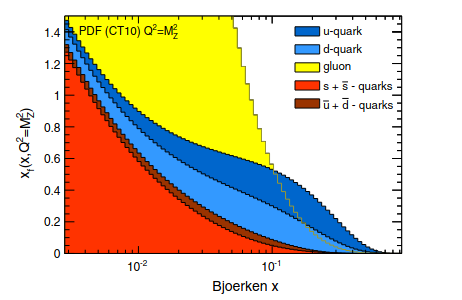
\includegraphics[scale=0.8]{chapter3/cteq-pdf.png}\\

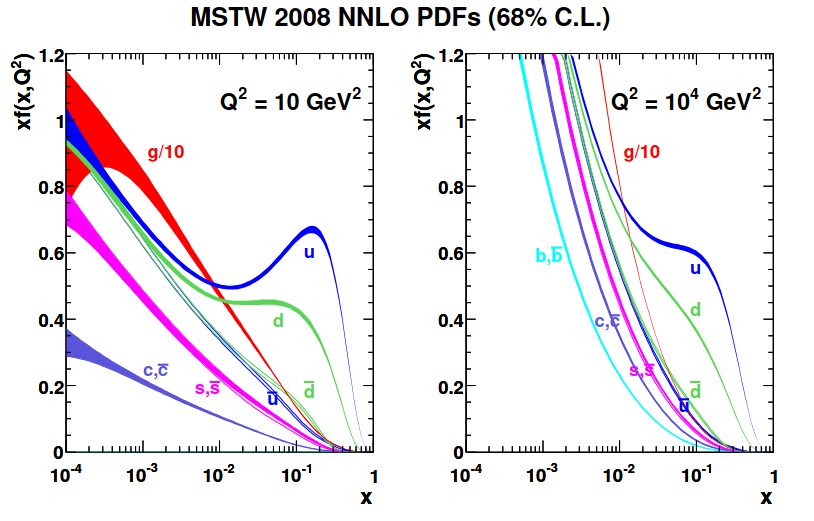
\includegraphics[scale=0.5]{chapter3/pdf1.png}
\end{tabular}
\caption{Parton Distribution Function evaluated at $Q^{2}=m_{Z}^{2}$~\textit{top}~\cite{Schott_2014}, MSTW 2008 NNLO PDFs at $Q^{2} = 10 GeV^{2} $and $Q^{2} = 10^{4} GeV^{2}$~\textit{bottom}~\cite{Martin_2009}}
\label{pdf-fit}
\end{figure}

There are several groups who performed PDFs fitting. The results of CTEQ~\cite{Nadolsky_2008}, MSTW~\cite{Martin_2009}, ABKM~\cite{Alekhin_2010} and NNPDF~\cite{Ball:2011us} collaborations some of which are shown in Fig.~\ref{pdf-fit}, use all available data for their fits. There are several assumptions and model uncertainties on which PDF approach and fitting is based.\\
There are different multi purpose event generators, which include all the theoretical aspects of the proton-proton collision. These events generators use different theoretical models which include, shower model for initial and final MPI model~\cite{Blok_2016} and hadronisation and final decay model. Some frequently used generators are PYTHIA~\cite{Sj_strand_2008}, HERWIG~\cite{Corcella_2001}, SHERPA~\cite{Gleisberg_2009} and POWHEG~\cite{Oleari_2010}. These generators have all aspects of Standard Model and new physics. The detail of each generator, and what it can do can be found in~\cite{Schott_2014}. 

\section{Measurement of Cross Section at The LHC}
Experimentally, the production cross section is measured by the following equation:
\begin{equation}
\sigma_{V}^{inc}=\frac{N_{signal}}{\epsilon.BR.\int \mathcal{L}dt}
\end{equation}
where $N_{signal}=N_{data}-N_{bkg}$ which is number of signal events, $N_{data}$ is the number of selected events from data and $N_{bkg}$ are the background events. The factor $\epsilon$ depends on determination of criteria for the signal selection. To specify the decay channel of $W$ and $Z$ boson branching ratio factor~(BR) is used. Integrated luminosity $\int \mathcal{L}dt$, tells about the size of data sample used.\\
The $\epsilon$ is defined as :
\begin{equation}
\epsilon=\frac{N_{reco.}^{selected}}{N_{gen.}^{all}}
\end{equation}
\begin{equation}
\epsilon=\frac{N_{reco.}^{selected}}{N_{gen.}^{selected}}.\frac{N_{gen.}^{selected}}{N_{gen.}^{all}}
\end{equation}
\begin{equation}
\epsilon=C.A
\end{equation}
where $N_{reco.}^{selected}$ are events selected at the reconstruction level and $N_{gen.}^{all}$ is the number of all generated events. $A$ represents fiducial acceptance factor and $C$ is for detector-induced correction factor. Ratio of the number of selected events at generator level~($N_{gen.}^{selected})$ to the total number of generated events~($N_{gen.}^{all}$)~ is called fiducial acceptance. The main source of uncertainties in the fiducial acceptance are scale and PDF uncertainties.\\
The detector correction factor $C$ is ratio of~($N_{reco.}^{selected}$) from data sample to the number of selected events~($N_{gen.}^{selected}$) from Monte Carlo. The dominant uncertainties in the detector correction factor are experimental sources.
The fiducial cross-section, defined as:
\begin{equation}
\sigma_{V}^{fid}=\frac{N_{data}-N_{bkg}}{C.BR.\int \mathcal{L}dt}=\sigma_{V}^{inc}.A
\end{equation}  
\section{Event Selection for Vector Bosons}
\subsubsection{ATLAS}
Events for $Z$ boson, i.e., $Z~\rightarrow~l^{+}l^{-}$ required Di lepton invariant mass of $66~GeV<~m_{ll}<116~GeV$. Muons must be in $|\eta|<2.4$ with $p_{T}(min.)~>~20~GeV$. Electrons are required to fulfill $1.52~<~|\eta|~<~2.4$ with $E_{T}(min.)>20GeV$.\\
$W$ boson decays to an energetic lepton and corresponding neutrino, neutrinos cannot be detected hence leads to missing transverse energy. Thus the mass of $W$ boson cannot be reconstructed due to this missing energy. The invariant mass projection to the transverse plane, defined as
\begin{equation}
m_{T}=\sqrt{2.p_{T}^{l}.p_{T}^{\nu}.(1-cos(\phi^{l}-\phi^{\nu}))}
\end{equation} 
can be reconstructed, where $p_{T}^{l}$ is lepton transverse momentum and $p_{T}^{\nu}$ is neutrino transverse momentum, $\phi^{l}$ and $\phi^{\nu}$ are azimuthal angles for lepton and neutrino respectively. For the $W$ boson events selection at ATLAS required one reconstructed, single lepton with $E_{T}^{miss.}$ of $25~GeV$ and $m_{T}(min.)~>~50~GeV$. Selection for the $Z$ boson by ATLAS is shown in Fig.~\ref{ATLAS_sel}
\begin{figure}[H]
\begin{tabular}{cc}

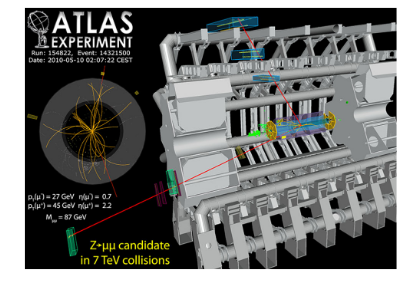
\includegraphics[scale=0.5]{chapter3/atlas.png}
&
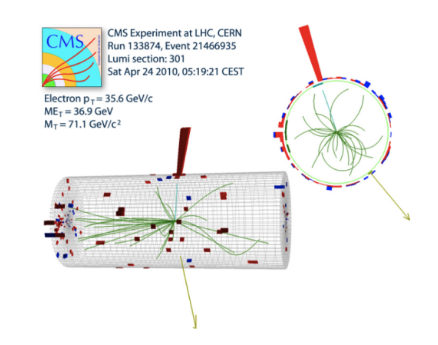
\includegraphics[scale=0.5]{chapter3/cms-w.png}
\end{tabular}
\caption{$Z\rightarrow \mu\mu$ in ATLAS detector~(left)~and $W\rightarrow e\nu$ in CMS detector~(right)~\cite{Schott_2014}.}
\label{ATLAS_sel}
\label{W-event}
\end{figure}
 
\subsubsection{CMS}
For $Z\rightarrow \mu\mu$, oppositely charged muons are required for $|\eta|<2.1$ and transverse momentum requirement of $p_{T}>20GeV$. For the electron decay channel $Z\rightarrow ee$, $|\eta|<1.44$ and $E_{T}>20$ GeV are required.\\
The selection criterion for $W$ boson events, required single electron with $E_{T}>25~GeV$ and $|\eta|<2.5$ or single muon with $p_{T}>25~GeV$ and $|\eta|<2.1$. A typical $W\rightarrow e\nu$ event in the CMS detector is shown in Fig.~\ref{W-event}. Tables \ref{Atlas_tab} and \ref{Cms_tab} show the kinematic cuts used by CMS and ATLAS.

\begin{table}[h!]
\centering
\caption{Kinematic cuts for CMS analysis~\cite{2011} at $7~TeV$ for leptonic channel of $Z$ and $W$ boson respectively.}
\begin{tabular}{|lp{5cm}p{5cm}|}
\hline
CMS&&\\
Electron-channel&$Z\rightarrow l^{+}l^{-}$ & $W\rightarrow l^{\pm}\nu$\\
\hline
&$E_{T}(e^{+})>25GeV$&one $ e^{\pm}$ with $E_{T}>25GeV$\\
&$E_{T}(e^{-})>25GeV$&$|\eta_{e^{\pm}}|<1.44$\\
&$|\eta_{e^{\pm}}|<1.44$&\\
&$60~GeV<m_{ee}<120~GeV$&\\
Muon-channel&&\\
\hline
&$p_{T}(\mu^{+})>25GeV$&one $ e^{\pm}$ with $p_{T}>25GeV$\\
&$p_{T}(\mu^{-})>25GeV$&$|\eta_{\mu^{\pm}}|<2.1$\\
&$|\eta_{\mu^{\pm}}|<2.1$&\\
&$60~GeV<m_{\mu\mu}<120~GeV$&\\
\hline
\end{tabular}
\label{Atlas_tab}
\end{table}

\begin{table}[h!]
\centering
\caption{Kinematic cuts for ATLAS analysis~\cite{Aad_2016} at $13~TeV$ for the leptonic channel of $Z$ and $W$ boson respectively.}
\begin{tabular}{|lp{5cm}p{5cm}|}
\hline
ATLAS&&\\
Electron-channel&$Z\rightarrow l^{+}l^{-}$ & $W\rightarrow l^{\pm}\nu$\\
\hline
&$E_{T}(e^{+})>25GeV$&$p_{T}^{(e^{\pm})}>25GeV$\\
&$E_{T}(e^{-})>25GeV$&$p_{T}^{(\nu)}>25Gev$\\
&$|\eta_{e^{\pm}}|<1.37$&$|\eta_{e^{\pm}}|<1.52$\\
&$66~GeV<m_{ee}<116~GeV$&$m_{T}>50GeV$\\
Muon-channel&&\\
\hline
&$p_{T}(\mu^{+})>25GeV$&$p_{T}^{(\mu^{\pm})}>25GeV$\\
&$p_{T}(\mu^{-})>25GeV$&$p_{T}^{(\nu)}>25GeV$\\
&$|\eta_{\mu^{\pm}}|<2.4$&$|\eta_{\mu^{\pm}}|<2.4$\\
&$66~GeV<m_{\mu\mu}<116~GeV$&$m_{T}>50GeV$\\
\hline
\end{tabular}
\label{Cms_tab}
\end{table}

\begin{figure}[h!]
\centering
\begin{tabular}{c}
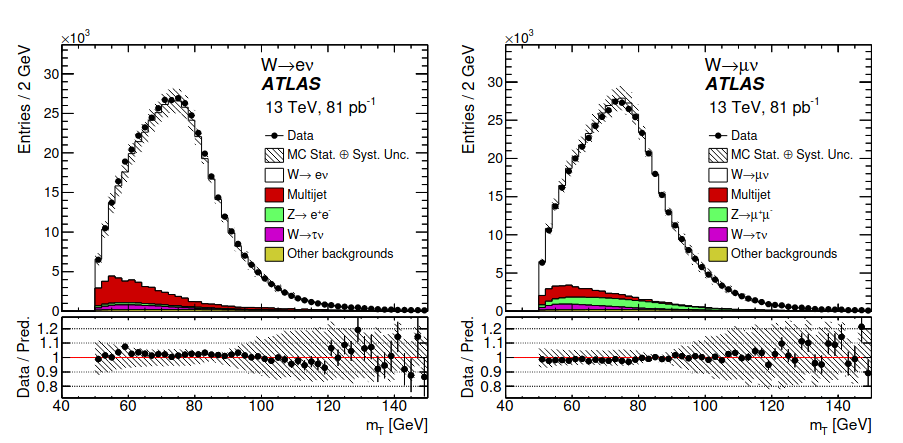
\includegraphics[scale=0.45]{chapter3/mt.png}\\

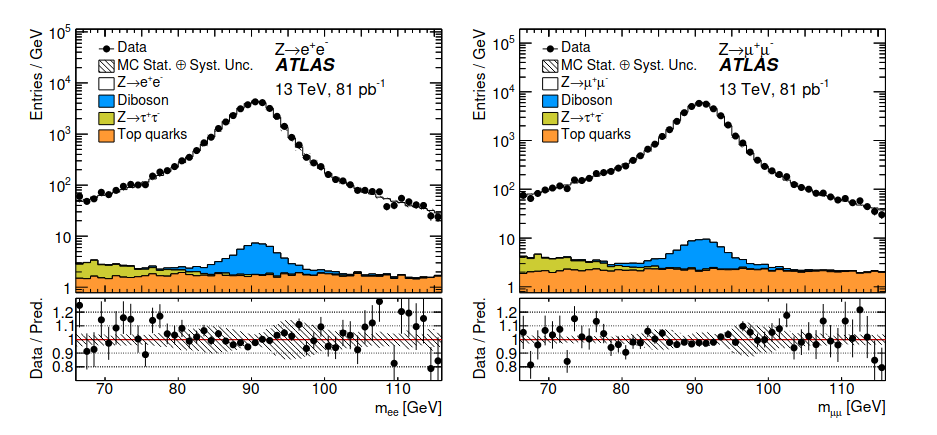
\includegraphics[scale=0.45]{chapter3/mll.png}
\end{tabular}
\caption{Transverse mass~$m_{t}$ distributions of $W\rightarrow e\nu$ and $W\rightarrow \mu\nu$ process~(top) and dilepton mass~$m_{ll}$ distribution~ (bottom)~\cite{Aad_2016}}
\label{mt_mll}
\end{figure}

The transverse mass distribution for electron and lepton channel of $W$ boson event and dilepton mass distribution for the $Z$ boson event can be seen in Fig.~\ref{mt_mll}. 
\section{Inclusive Cross Section of $W$ and $Z$ Bosons  }
For the Drell–Yan processes~\cite{Peng:2016ebs} as shown in Fig.~\ref{drell-yan}, the theoretical prediction at NNLO are known in term of $\alpha_{s}$~(strong coupling constant) for the inclusive production cross section of  the $Z$ and $W$ vector boson.\\
$Z$ bosons are produced by the quarks-antiquark annihilation, i.e. $u\overline{u}$, $d\overline{d}$ and also $s\overline{s}$. $W^{\pm}$ boson production is different from $Z$ boson because it depends on the charge of $W$, $W^{+}$ boson is produced in $u\overline{d}\rightarrow W^{+}$ process and $W^{-}$ in $d\overline{u}\rightarrow W^{-}$ process. $W^{+}$ is produced from the annihilation of $u-$valance quarks and $\overline{d}-$sea quark, $W^{-}$ from $d-$valance quark and $\overline{u}$ quark. Since there are two $u-$ quarks~(valance) and one $d-$ quark~(valance) available in the proton, therefore more $W^{+}$ bosons are expected than $W^{-}$ bosons. Thus QCD predictions can be tested precisely from the ratio of  $W^{+}$ and $W^{-}$ production as cross section ratios cancel many of the theoretical and experimental uncertainties.\\
\begin{figure}[H]
\begin{tabular}{c}
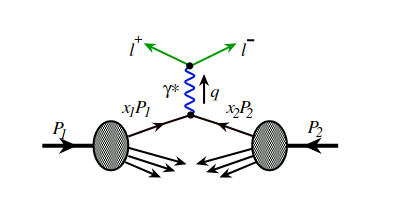
\includegraphics[scale=0.5]{chapter3/drell-yan1.png}
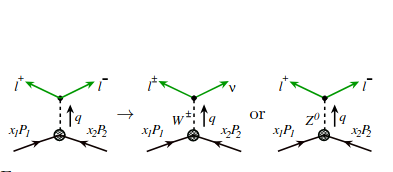
\includegraphics[scale=0.5]{chapter3/drell-yan2.png}
\end{tabular}
\caption{Graphical sketch for the generalized partonic
hard part of the Drell-Yan process~\cite{Peng:2016ebs}}
\label{drell-yan}
\end{figure}
Integrated luminosity is one of the main source of experimental uncertainties. In cross-section ratio measurement, this uncertainty is reduced, along with some other experimental and theoretical uncertainties.~Therefore along with cross-section of $W$ and $Z$ boson, cross section ratios $\frac{\sigma(W^{+}+\sigma(W^{-})}{\sigma(Z)}$ and $\frac{\sigma(W^{+})}{\sigma(W^{-})}$, have unique importance.\\
The cross-section ratio for $\sigma(W^{+}+W^{-})/\sigma(Z)$ represents the cross section dependence on the quarks-distribution functions.
 
 \begin{eqnarray}
\sigma(W^{+}+\sigma(W^{-})=u_{v}(x)+\overline{d}_{v}(x)+d_{v}(x)+\overline{u}_{s}(x)\\
\sigma(Z)=(g_{V}(u)^{2}+g_{A}(u)^{2}.u_{q}(x))+(g_{V}(d)^{2}+g_{A}(d)^{2}.v_{q}(x))
\end{eqnarray} 
with\\

\begin{equation}
u_{q}(x)=(u_{v}(x)+\overline{u}_{s}(x))
\end{equation}
\begin{equation}
v_{q}(x)=(d_{v}(x)+\overline{d}_{s}(x))  
\end{equation}
where $u_{v}(x)$ and $\overline{u}_{s}(x)$ are valance quark distributions and $u_{s}(x)$ and $d_{s}(x)$ are the respective sea-quark distributions.
If we assume that light sea quark and anti-quark have same distribution, then the PDF dependence will be reduced,~i.e, $\overline{q}(x) = q(x)$  for $q= u,d,s..$. Thus the ratio of $W$ to $Z$ boson helps us to constrain the strange quark distribution~\cite{Aad_2012}.\\
The above statement doesn't hold for cross-section ratios, such as ratio of $W^{+}$ to $W^{-}$, $W^{+}$ or $W^{-}$ to $Z$ boson. These cross section ratios have a large dependence on difference in the $u-$ and $d-$quark distribution functions, and is very sensitive to this difference in valance-quark distributions. However, for the PDFs constraints, along with inclusive cross section the differential cross section measurements are also very important. 

\subsection{Differential Production Cross Section of $W$ and $Z$ Boson:}
The differential cross section also measured at LHC with great precision, and differential cross section of vector bosons plotted versus their rapidity distribution, provides extra constraint on the PDFs.

Rapidity distribution for the process $Z\rightarrow l^{+}l^{-}$, can be directly measured from  detector data, because  four-momenta of the decaying leptons can be precisely measured and thus rapidity can be measured precisely. This will help us to constrain the PDFs of $u\overline{u}$, $d\overline{d}$, and $s\overline{s}$. The differential cross section measurement helps us to improve strange-quark PDFs. Fig.~\ref{raptdity-atlas} shows different quark/antiquark annihilation processes for different rapidity ($y_{Z}$) values.  The rapidity distribution of $Z$ boson from the annihilation of $u\overline{u}$, $d\overline{d}$ and $s\overline{s}$ processes gives additional constraints on PDFs, as well as the rapidity distribution in the central region for $s\overline{s}$ process, is important to determine its PDFs. 
ATLAS and CMS both, published differential cross section $\frac{d\sigma}{d|y_{z}|}$ for different integrated luminosities $\int\mathcal{L}dt$ in the fiducial region defined by kinematic cuts earlier.\\
The $W$ boson decays into lepton and corresponding neutrino,~i.e.,~$W^{\pm}\rightarrow l^{\pm}\nu$. The direct measurement of rapidity distribution of $W^{\pm}$ boson is not possible, because the $p_{z}$ of decayed neutrino can't be reconstructed, thus pseudo rapidity of the decay lepton $\eta_{l}$ is measured and correlated to $y_{W}$ by an indirect method.
The rapidity distribution of $W^{\pm}$ boson is sensitive to the $u\overline{d}$ and $d\overline{u}$~quark distribution as shown in Fig.~\ref{raptdity-atlas}. The $y_{Z}$ measurement helps us to constrain the PDFs of strange quark.\\
Differential cross-section measurements of the $W$ and $Z$ bosons provide important constraints for the PDFs. Fig.~\ref{ubsr-sbsr} shows the difference in  PDFs of $\overline{u}$ and $\overline{s}$ quarks with and without LHC data based on the NNPDF group.
\begin{figure}[H]
\centering
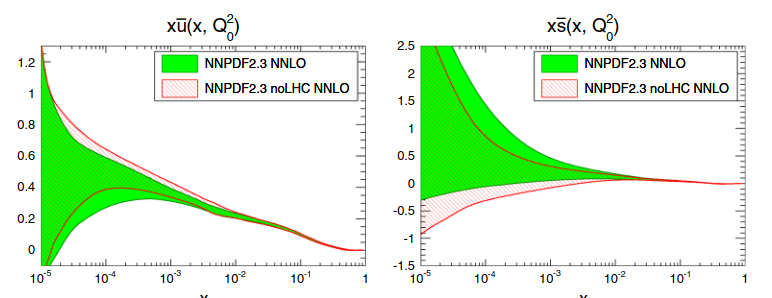
\includegraphics[scale=0.5]{chapter3/strange-quark.png}
\caption{Comparison of PDfs of $\overline{u}$ and $\overline{s}$~quark with LHC and without LHC data.~\cite{Schott_2014}. Comparison plots can also be found in~\cite{Ball_2013}.}
\label{ubsr-sbsr}
\end{figure}

\begin{figure}[H]
\centering
\begin{tabular}{c}
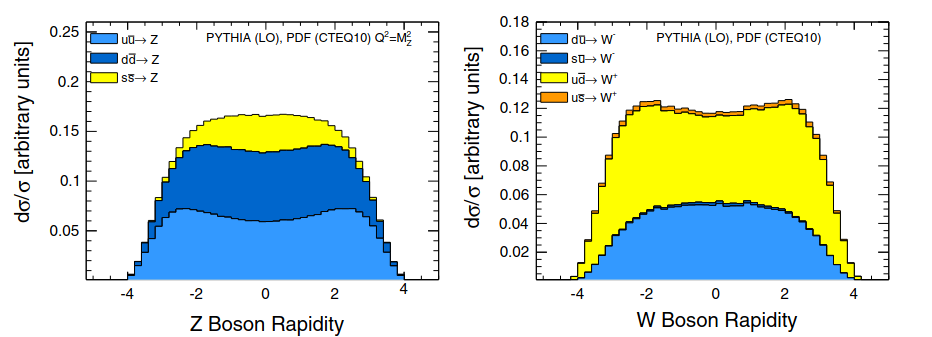
\includegraphics[scale=0.44]{chapter3/rapidity.png} \\
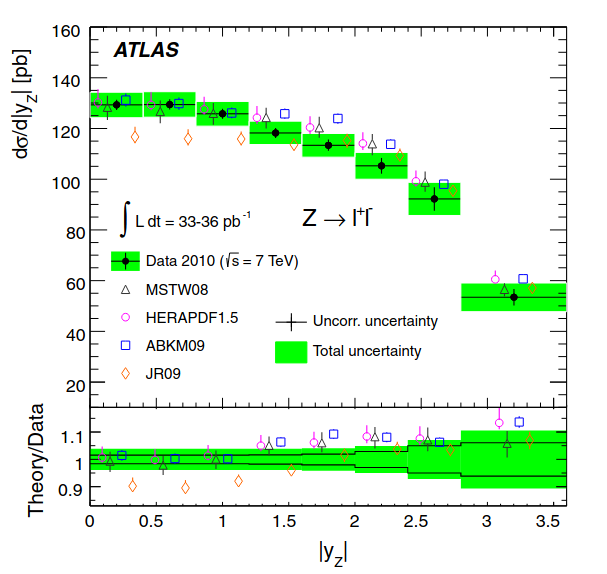
\includegraphics[scale=0.44]{chapter3/atlas-rapidity.png}
\end{tabular}
\caption{$Z$ boson rapidity distribution~(\textit{left}) and $W$ boson rapidity distribution~(\textit{right}) in 7 TeV pp collisions(\textit{top}), for $Z\rightarrow l^{+}l^{-}$ the combined $d\sigma/d|y_{Z}|$ cross-section measurement compared to NNLO theoretical predictions (\textit{bottom})~ \cite{Schott_2014}}.
\label{raptdity-atlas}
\end{figure} 


\section{Measurement of $p_{T}$ of Vector Bosons}
The $W$ boson mass at LHC can be measured by the accurate measurement and understanding of transverse momentum $p_{T}$, the $p_{T}$ distribution of product leptons of $W^{\pm}~\rightarrow~l^{\pm}\nu$ is an important parameter for $m_{W}$.\\
The $p_{T}$ distribution of electron and muon channel for the $Z\rightarrow l^{+}l^{-}$ process can be computed directly from four momentum information of resulting leptons.\\
The $p_{T}(Z)$ distribution is a important tool for the Monte-Carlo~(MC) generators, and transverse momentum of $Z$ boson helps to measure the $p_{T}(W)$, of which direct measurement is not possible.
The transverse momentum of  $W$ boson cannot be measured directly from the decayed leptons because we don't know about neutrino momentum. However, the $p_{T}~(W)$ is measured by the $p_{T}~(hadron)$ from which it was produced. The $p_{T}~(W)$ is balanced by the hadronic transverse momentum $p_{T}~(hadron)$, i.e.
\begin{equation}
p_{T}(W)=-p_{T}(had)=p_{T}(l^{\pm}+p_{T}(\nu)),
\end{equation}
where $p_{T}(had)$ is the recoil of hadron~(Fig. \ref{pt-w}),
\begin{figure}[h!]
\centering
\begin{tabular}{c}
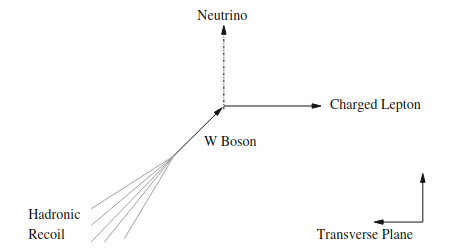
\includegraphics[scale=0.8]{chapter3/pt.png}\\
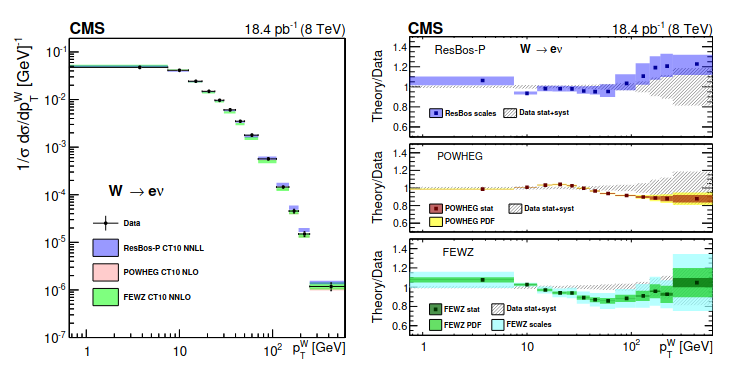
\includegraphics[scale=0.5]{chapter3/ptw.png}
\end{tabular}
\caption{Hadronic recoil illustration in $W^{\pm}~\rightarrow~ l^{\pm}\nu$ events~(\textit{top}). Differential cross sections~(Normalized) for $W$ boson as a function of $p_{T}~(W)$ for electron. Ratios of theoretical predictions to the data~(\textit{bottom}) ~\cite{Khachatryan_2017}.}
\label{pt-w}
\end{figure}
hence $p_{t}(W)$ can be measured from hadronic transverse momentum $p_{t}(hadron)$, which is due to hadronic activities in QCD interactions of hadrons. Due to several experimental uncertainties in the hadronic recoil, a theoretical model is used to define the relation between $p_{T}(had)$ and $p_{T}(W)$. Data of $Z$ boson events helps to model this theoretical model. We consider that the hadronic recoil $p_{T}~(hadron)$ is same for the $W$ and $Z$ bosons, and with different approach we can find $p_{T}~(W)$.

\section{Measured Cross Section of $W$ and $Z$ Bosons at Different C.O.M Energy}
The production cross section of $W$ and $Z$ vector bosons is measured at LHC in ATLAS and CMS experiments at different center-of-mass energies,~i.e., $7~TeV$, $8~TeV$ and $13~TeV$  with certain uncertainties~($\pm stat.\pm syst.\pm lumi.$). The measured value of cross section increased with the increase in center-of-mass energy as shown in Fig.~\ref{pred-inc}.
\begin{figure}[h!]
\centering
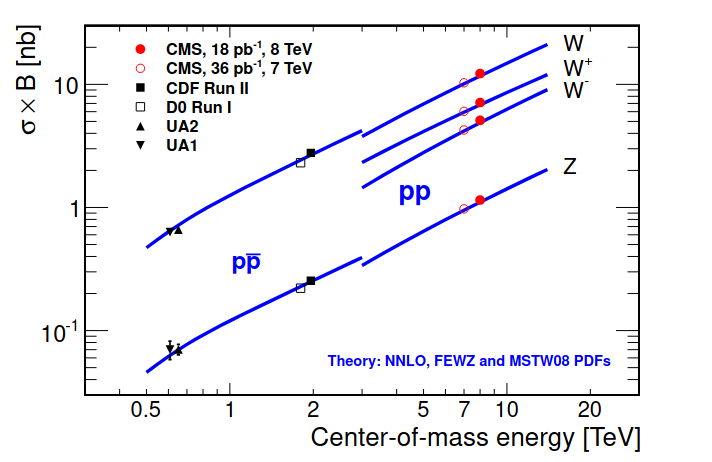
\includegraphics[scale=0.5]{chapter3/cross-sction-inc.png}
\caption{The predicted increase in cross section of vector bosons~\cite{Chatrchyan_2014}.}
\label{pred-inc}
\end{figure}
The production cross-section of $W$ and $Z$ boson, measured~$(\sigma\times BR(W\rightarrow l\nu, Z\rightarrow ll))$ and predicted at various c.o.m energies is listed in the following Tables \ref{7_1},~\ref{7_2},~\ref{8_1},~\ref{8_2},~\ref{13_1} and \ref{13_2}.


\begin{table}[H]
\caption{Measured and NNLO predicted Ratios of $W^{+}/W^{-}$ and $W^{\pm}/Z$. The measured values are at $7~TeV$ with an integrated luminosity of $36~pb^{-1}$ at CMS~\cite{2011}.}
\centering
\begin{tabular}{|l|p{6cm}|p{6cm}|}
\hline
Channel&\bf Measured Ratio&\bf Predicted Ratio (NNLO) (value$\pm$PDF)\\
\hline
\hline
$W^{+}/W^{-}$&1.418~$\pm$~0.008~$\pm$~0.02&1.43~$\pm$~0.001\\
$W^{\pm}/Z$&10.56$\pm$0.12$\pm$0.12&10.47$\pm$0.04\\
\hline
\label{7_1}
\end{tabular}

\end{table}

\begin{table}[H]
\caption{The measured total $\sigma^{tot}$ cross section for leptonic channel of $W^{-}$, $W^{+}$, $W^{\pm}$ and $Z-$boson, and predicted total cross section. The measured values with certain uncertainties~($~\pm~stat.~\pm~ syst.~\pm~ lumi.$) are at $7~TeV$ with integrated luminosity $36~pb^{-1}$ at CMS and the predictions are at NNLO~\cite{2011}.}
\centering
\begin{tabular}{|l|p{6cm}|p{6cm}|}
\hline
\bf channel&\bf Measured Cross section~[nb]&\bf Predicted Cross Section (NNLO)~[nb] (value$\pm$PDF)\\
\hline
\hline
$W^{-}$&4.34~$\pm$~0.02~$\pm$~0.11~$\pm$~0.25&4.29~$\pm$~0.11\\
$W^{+}$&6.115~$\pm$~0.02~$\pm$~0.07~$\pm$~0.24&6.15~$\pm$~0.17\\
$W^{\pm}$&10.48~$\pm$~0.03~$\pm$~0.16~$\pm$~0.43&10.44~$\pm$~0.27\\
\hline
\hline
$Z$&0.99~$\pm$~0.011~$\pm$~0.02~$\pm$~0.03&0.97~$\pm$~0.03\\
\hline
\end{tabular}
\label{7_2}
\end{table}


\begin{table}[H]
\caption{The measured total $\sigma^{tot}$ cross sections with uncertainties~($~\pm~ stat.~\pm~ syst.~\pm~ lumi.$) for lepton channels of $W^{-}$, $W^{+}$, $W^{\pm}$ and $Z-$boson, and predicted total cross section. The measured values are at $8~TeV$ with integrated luminosity $18.2~pb^{-1}$ at CMS and predictions are at NNLO~\cite{Chatrchyan_2014}.}
\centering
\begin{tabular}{|l|p{6cm}|p{6cm}|}
\hline
channel&\bf Measured Cross section~[nb]&\bf Predicted Cross section~[nb] (value$\pm$PDF)\\
\hline
\hline
$W^{-}$&5.09~$\pm$~0.02~$\pm$~0.11~$\pm$~0.18&5.06~$\pm$~0.13\\
$W^{+}$&7.11~$\pm$~0.03~$\pm$~0.14~$\pm$~0.13&7.12~$\pm$~0.20\\
$W^{\pm}$&12.21~$\pm$~0.02~$\pm$~0.55~$\pm$~0.43&12.18~$\pm$~0.32\\
\hline
\hline
$Z$&1.15~$\pm$~0.01~$\pm$~0.02~$\pm$~0.03&1.13~$\pm$~0.04\\
\hline
\end{tabular}
\label{8_1}
\end{table}

\begin{table}[H]
\caption{Measured and predicted Ratios $W^{+}/W^{-}$ and $W^{\pm}/Z$. The measured values are at $8~TeV$ with integrated luminosity $18.2~pb^{-1}$ at CMS and predictions are at NNLO~\cite{Chatrchyan_2014}.} 
\centering
\begin{tabular}{|l|p{6cm}|p{6cm}|}
\hline
Channel&\bf Measured Ratio\newline(Value$\pm$stat.$\pm$syst.)&\bf Predicted Ratio(NNLO)\newline(value$\pm$PDF)\\
\hline
\hline
$W^{+}/W^{-}$&1.395~$\pm$~0.01~$\pm$~0.020&1.418~$\pm$~0.02\\
$W^{\pm}/Z$&10.63~$\pm$~0.11~$\pm$~0.25&10.47~$\pm$~0.04\\
\hline
\end{tabular}
\label{8_2}
\end{table}

\begin{table}[H]
\caption{The measured total $\sigma^{tot}$ cross sections for the lepton channel of $W^{-}$, $W^{+}$, $W^{\pm}$, and $Z-$boson, and predicted total cross section. The measured values are at $13~TeV$ with integrated luminosity $43~pb^{-1}$ at CMS~\cite{CMS:2015ois}.}
\centering
\begin{tabular}{|l|p{6cm}|p{6cm}| }
\hline
\bf channel&\bf Measured Cross section[nb] &\bf Predicted Cross section~[nb] (NNLO) (value$\pm$PDF$\pm$scale $\pm$ other)\\
\hline
\hline
$W^{-}$&8.68~$\pm$~0.08~$\pm$~0.25~$\pm$~0.42&$8.37_{-0.21}^{+0.24}~\pm$~0.11~$\pm$~0.12\\
$W^{+}$&11.39~$\pm$~0.09~$\pm$~0.34~$\pm$~0.55&$11.33_{-0.27}^{+0.24}~\pm$~0.15~$\pm$~0.16\\
$W^{\pm}$&20.07~$\pm$~0.12~$\pm$~0.57~$\pm$~0.96&$19.7_{-0.47}^{+0.56}~\pm$~0.26~$\pm$~0.28\\
\hline
\hline
$Z$&1.92~$\pm$~0.02~$\pm$~0.06~$\pm$~0.09&1.87~$\pm$~0.05~$\pm$~0.03~$\pm$~0.03\\
\hline
\end{tabular}
\label{13_1}
\end{table}

\begin{table}[H]
\caption{Measured and predicted Ratios $W^{+}/W^{-}$ and $W^{\pm}/Z$. The measured values are at $13~TeV$ with integrated luminosity $43~pb^{-1}$\cite{CMS:2015ois}.} 
\centering
\begin{tabular}{|l|p{6cm}|p{6cm}|}
\hline
\bf Channel&\bf Measured Ratio\newline(Value$\pm$stat$\pm$syst)&\bf Predicted Ratio(NNLO)\newline(value$\pm$PDF)\\
\hline
\hline
$W^{+}/W^{-}$&1.31~$\pm$~0.02~$\pm$~0.03&1.35~$\pm$~0.01\\
$W^{\pm}/Z$&10.46~$\pm$~0.06~$\pm$~0.16&10.55~$\pm$~0.07\\
\hline
\end{tabular}
\label{13_2}
\end{table}

\begin{figure}[H]
\centering
\begin{tabular}{c}
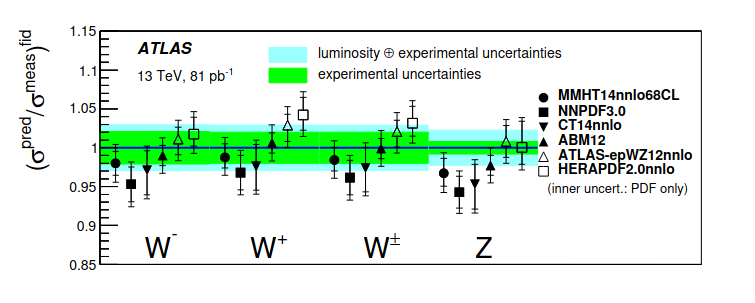
\includegraphics[scale=0.57]{chapter3/atlas13.png}\\
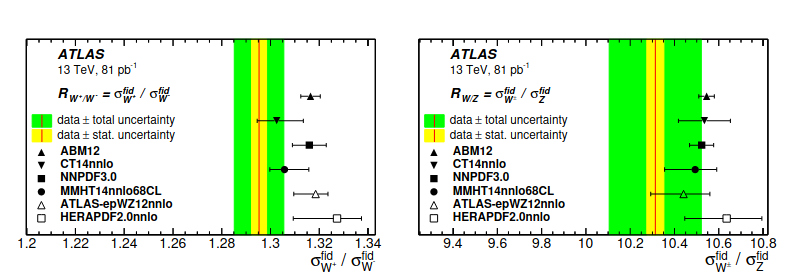
\includegraphics[scale=0.5]{chapter3/atlas13-1.png}
\end{tabular}
\caption{Ratio of Measured to predicted cross section(\textit{top}), comparison of measured and predicted cross section ratio of $W$ and $Z$ boson~(\textit{bottom}).~\cite{Aad_2016} }
\label{ratio-13tev}
\end{figure}


\begin{figure}[H]
\centering
\begin{tabular}{c}
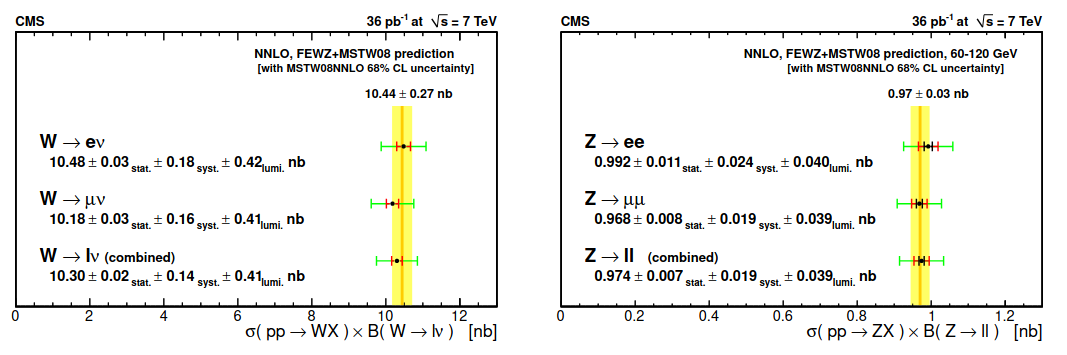
\includegraphics[scale=0.4]{chapter3/7tev1.png}\\
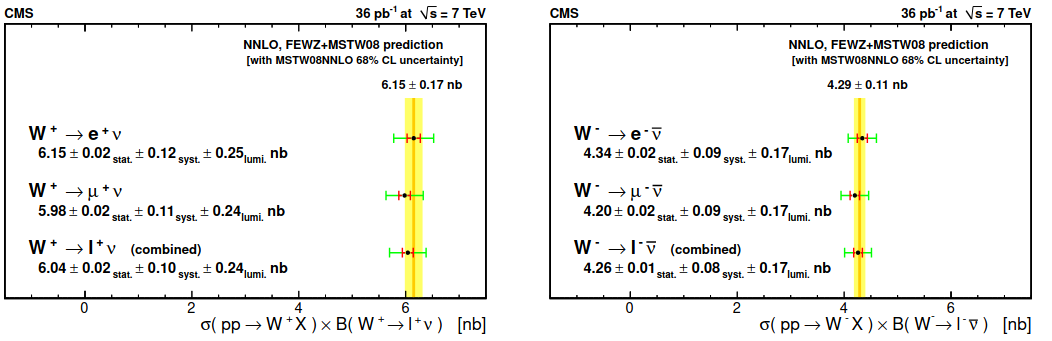
\includegraphics[scale=0.4]{chapter3/7tev2.png}\\
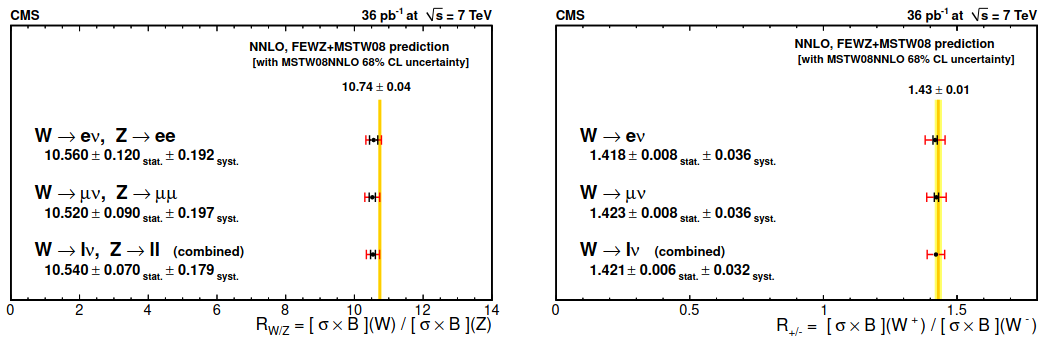
\includegraphics[scale=0.4]{chapter3/7tev3.png}
\end{tabular}
\caption{Measurements of vector boson cross section production multiplied with leptonic branching ratio~\textit{(top)}. Measurements of $W^{+}$ and $W^{-}$ production cross section times branching ratio~\textit{(middle)}. Ratio of $W^{+}$ to $Z$ and $W^{+}$ to $W^{-}$~\textit{bottom}. The yellow line showing the measured value with various experimental uncertainties at $7~TeV, 36~pb^{-1}$~\cite{2011}}
\label{7tev.data}
\end{figure}

Fig. \ref{ratio-13tev} shows the ratio of the experimentally measured and theoretically predicted cross section for the leptonic channel~($e$ and $\mu$) using various PDFs and also ratio of  production cross section of charged $W$ boson and $W^{\pm}$ boson to $Z$ boson compared to theoretical predictions with different PDF sets.

Fig.~\ref{7tev.data} shows the summary of the measurement in the electron and muon channels by CMS at $7~TeV$, and results are compared with the theoretical predictions. 


\begin{figure}[H]
\centering
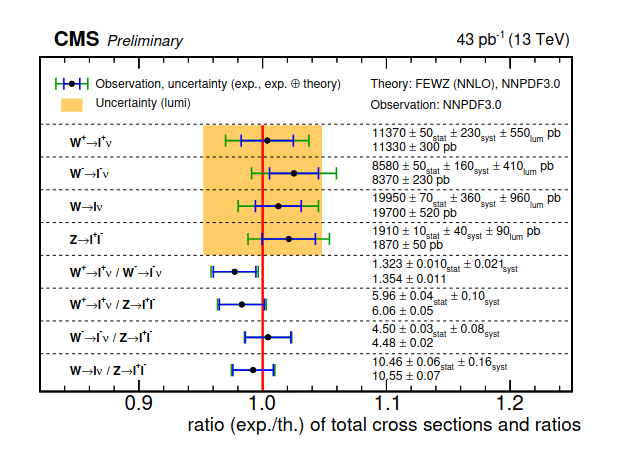
\includegraphics[scale=0.5]{chapter3/cms13.png}
\caption{The CMS measured total cross sections of $W$, $W^{+}$, $W^{-}$ and $Z$ boson times branching fraction and theoretically predicted cross section. In each column upper value represent measured cross section with uncertainties and lower value represent theoretically predicted cross section, and their ratio also.~\cite{CMS:2015ois}}       
\label{cms_comp}
\end{figure}
Figs.~\ref{cms_comp},~\ref{cms_comp1} and \ref{cms_comp2} shows the comparision of measurements at CMS with predictions by NNPDF3.0~(NNLO) at $13~TeV$.

\begin{figure}[H]
\centering
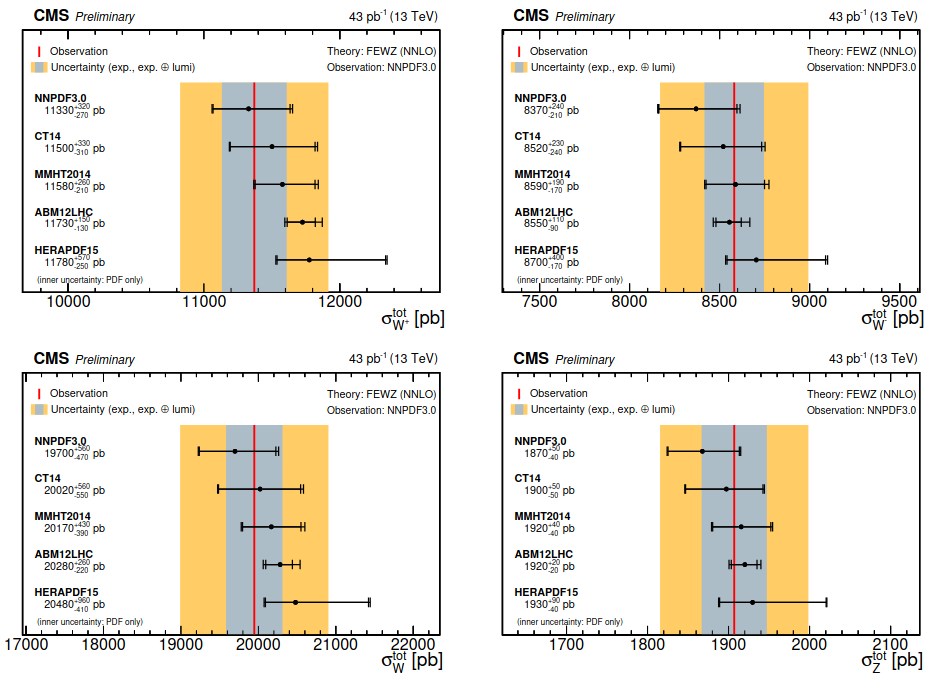
\includegraphics[scale=0.45]{chapter3/cms213.png}
\caption{Measured cross section ~(red line) and predicted cross section with different PDFs. The data points with error bars represent theoretically predicted value with various uncertainties~\cite{CMS:2015ois}}
\label{cms_comp1}
\end{figure}
\begin{figure}[H]
\centering
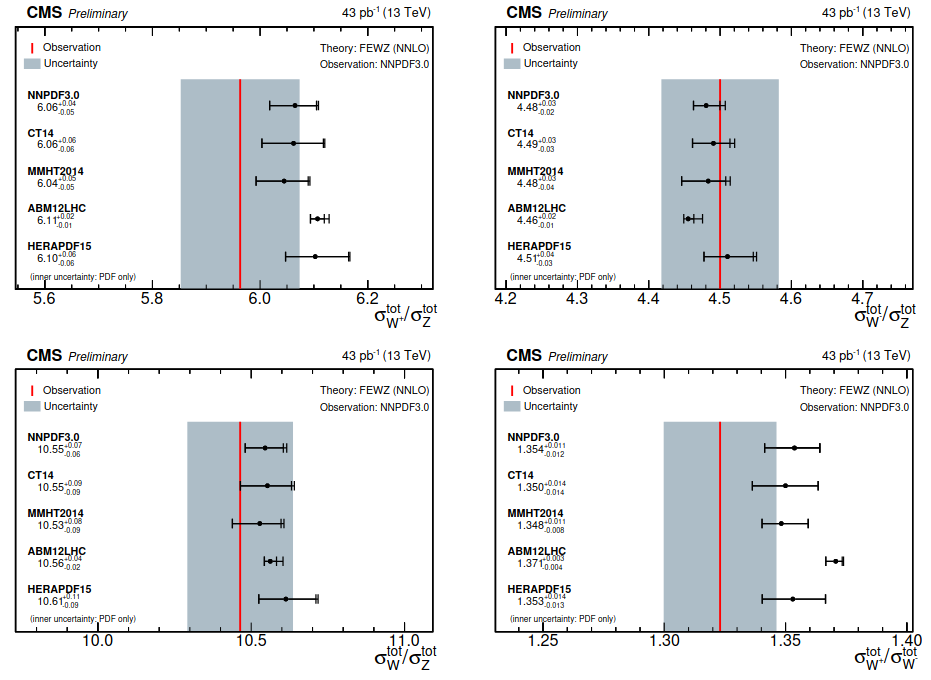
\includegraphics[scale=0.45]{chapter3/cms313.png}
\caption{Measured total  cross section ratios of vector bosons and predicted cross section ratios of vector boson with different PDFs set~\cite{CMS:2015ois}.}
\label{cms_comp2}
\end{figure}

\section{Uncertainties in the Predictions}
Imperfect knowledge of the proton parton distribution functions is the main source of uncertainties in predictions. The PDFs uncertainties can be evaluated from sum in quadrature by the difference of central PDF and Eigenvectors or error vectors of respective PDF set.\\
The uncertainties determination depends upon the given PDF set, for Monte Carlo set (NNPDF) uncertainties are determined differently from Hessian PDF  set and same for all other sets. 
\subsection{Computation of Hessian PDF uncertainties}
In hessian matrix approach the experimental uncertainties are propagated by diagonalising the $n\times n$ hessian matrix, more details can be found in~\cite{alekhin2011pdf4lhc}.

\textit{Hessian:} Consider a variable $Y$; the central value for $Y$ using central PDF is given by $Y_{0}$. $Y_{i}^{+}$ and $Y_{i}^{-}$ is the value of that variable corresponding to positive and negative direction of the error vector $i$ respectively~\cite{alekhin2011pdf4lhc}.  
\begin{eqnarray}
\Delta Y_{max}^{+}=\sqrt{\Sigma_{i=1}^{N}[max(Y_{i}^{+}-Y_{0},Y_{i}^{-}-Y_{0},0)]^{2}}\\
\Delta Y_{max}^{-}=\sqrt{\Sigma_{i=1}^{N}[max(Y_{0}-Y_{i}^{+},Y_{0}-Y_{i}^{-},0)]^{2}}
\end{eqnarray}
$\Delta Y^{+}$ is the PDF error which indicates increase in the observable $Y$, and $\Delta Y^{-}$ the PDF error indicates decrease in the observable $Y$. The sum is over all $N$ eigenvector directions.\\
\textit{Symmetric Hessian:} For the simple symmetric case where only the value of variable using central PDF $Y_{0}$ and $N$ error vector using PDF  $Y_{i}$, $(i = 1, . . . , N)$ are provided, the central value and PDF uncertainties are calculated as:
\begin{equation}
\Delta Y^{+}=\Delta Y^{-}=\Delta Y=\sqrt{\Sigma_{i=1}^{N}(Y_{i}-Y_{0})^{2}}
\end{equation}
\subsection{Computation of Monte Carlo PDF uncertainties}
For the NNPDF Monte Carlo set, a PDFs set with replicas is given. The average value for any observable $X$~(for example cross section) which depends on the PDFs sets is computed from usual formula:
\begin{equation}
<X(q)>~=~\frac{1}{N_{rep}}X_{i=1}^{N_{rep}}X(q^{i})
\end{equation}
where $N_{rep}$ is the number of replicas in the Monte Carlo PDF set. The associated uncertainty in the observable is found, according to the usual formula:
\begin{eqnarray}\label{sd}
\sigma_{X}~=~[\frac{N_{rep}}{N_{rep}-1}{\langle X(q)^{2}\rangle -\langle X(q)\rangle ^{2})}]^{1/2}\\
\sigma_{X}~=~[\frac{1}{N_{rep}-1}\Sigma_{i=1}^{N_{rep}}(X(q^{i})-\langle X(q) \rangle)^{2}]^{1/2}
\end{eqnarray}
NNPDF group provide both $N_{rep} = 100 $ and $N_{rep} = 1000$ replicas set. Equation \ref{sd} provides the 1–sigma PDF uncertainty on a general quantity which depends on PDFs.\\
Different PDFs groups provide both $68\%$ and $90\%$ confidence-level(C.L.) uncertainties. Some PDFs groups provide sets for both the $68\%$ confidence-level (C.L.) and $90\%$ C.L. Uncertainties. These uncertainties can be co-related by a factor of $1.64485$. In general we can evaluate PDFs uncertainties for both confidence level $68\%$ and $90\%$~i.e. NNPDF3.1~\cite{Watt_2011}.
\subsection{Theoretical Uncertainties}
The determination of theoretical uncertainties improves the PDFs relation to measurable quantities. The study of experimental uncertainties is much advanced than theoretical uncertainties, and only some of the theoretical uncertainties are explored in detail.\\
The determination ofstrong interactions between the quarks is the first source of theoretical uncertainty. The QCD parameters including the value of the strong coupling constant $\alpha_{s}$ and the heavy quark masses $m_{c}~(charm quarks)$ and $m_{b}~(bottom quark)$, and variation of re-normalisation $\mu_{R}$ and factorisation $\mu_{F}$ scales are the source of theoretical uncertainties.\\
Of these uncertainties, the uncertainty due to choice of strong coupling constant value $\alpha_{s}$ is explored in detail by each PDF group. The uncertainty due to choice of heavy quark masses~(charm and bottom) is also explored by some PDF groups~e.g. NNPDF3.1, Cteq18, HERA etc. The uncertainties due to variation in factorisation and re-normalisation scales are explored by NNPDF3.1.  
\subsubsection{The value of $\alpha_{s}$ ant its uncertainty}
The theoretical uncertainty due to the choice of strong coupling constant $\alpha_{s}$ value is studied and explored by each PDFs group. Different PDFs groups used different value of $\alpha_{s}$ as shown in Fig.~\ref{alpha}. The choice of $\alpha_{s}$ has clear importance for the PDFs prediction, especially for the gluons distribution.
\begin{figure}[H]
\centering
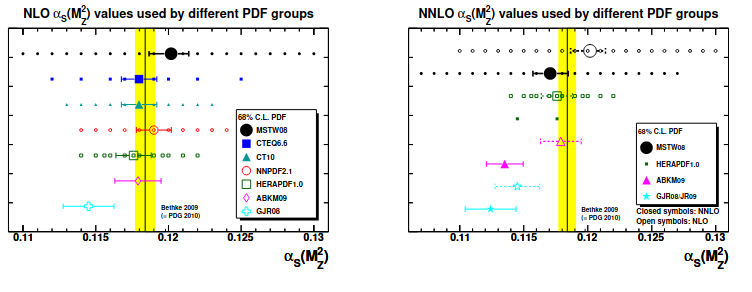
\includegraphics[scale=0.5]{chapter3/alpha.png}
\caption{The value of $\alpha_{s}$ used by different PDF groups}
\label{alpha}
\end{figure}
The values of $\alpha_{s}(m_{Z}^{2})$ and its uncertainties used by different PDFs  group are summarized in Fig.~\ref{alpha}. The world average value of $\alpha_{s}(m_{Z}^{2})$ is $\alpha_{s} = 0.1184 \pm 0.0007$~\cite{Martin_2009}.\\
The uncertainty on the value of $\alpha_{s}$, $\Delta\alpha_{s}=\pm0.001$ at $68\%$ C.L. and $\Delta\alpha_{s}=\pm0.002$ at $90\%$ C.L. has been used for the CTEQ, NNPDF studies. The predictions in the value of cross section changes with the choice of $\alpha_{s}$ value used. \\
\begin{figure}[h!]
\centering
\begin{tabular}{c}
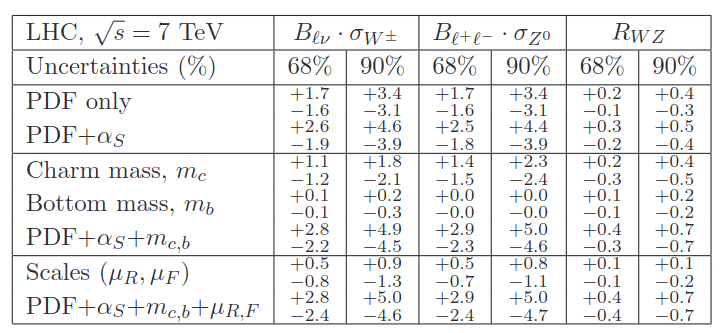
\includegraphics[scale=0.5]{chapter3/uncertain1.png}\\
\includegraphics[scale=0.5]{chapter3/uncertain2.png}
\end{tabular}
\caption{Summary of theoretical uncertainties in prediction of $W$ and $Z$ boson cross-sections at 7TeV~\cite{Watt_2011}}
\vspace{2cm}
\label{uncertain}
\end{figure}
Various theoretical uncertainties for the $7~TeV$ are shown in Fig.~\ref{uncertain}.
\subsubsection{Computation of PDF+$\alpha_{s}$ uncertainties}
If PDF uncertainty and the $\alpha_{s}(m_{Z}^{2})$ uncertainty are correlated then PDF$+\alpha_{s}$ uncertainty at $68\%$~C.L. or 1-$\sigma$ uncertainty can be calculated. First calculate the 1-$\sigma$ PDF uncertainty at fixed $\alpha_{s}$ value, and then compute 1-$\sigma$ uncertainty in $\alpha_{s}$ with PDFs fixed at their central value, 1-$\sigma$ change in $\alpha_{s}$ corresponds to the change of 0.001 in its value and 2-$\sigma$ corresponds to the change of 0.002.\\
For example, if $\Delta\sigma_{PDF}$ is the PDF uncertainty in the cross section $\sigma$ and $\Delta_{\alpha_{s}(m_{Z}^{2})}\sigma$ is the $\alpha_{s}$ uncertainty, the combined PDFs$+\alpha_{s}$ uncertainty in $\Delta_{\sigma}$ is
\begin{equation}
\Delta\sigma~=~\sqrt{\Delta\sigma_{PDF}^{2}+\Delta\sigma_{\alpha_{s}}^{2}}
\end{equation}
Different PDFs groups used different strategies for computation of PDF+$\alpha_{s}$ uncertainty.
\subsubsection{NNPDF-Combined PDF and $\alpha_{s}$ uncertainties:}
For NNPDF3.1 PDFs, PDF set are given with value $\alpha_{s}$ in the range from 0.108 to 0.124 in step of $\Delta\alpha_{s}=0.002$ and few are also given with step of 0.001, for cross section which depends on the PDFs and the strong coupling  $\sigma(PDF, \alpha_{s})$, we have\\
\begin{equation}
(\delta\sigma)_{\alpha_{s}}^{\pm}~=~\sigma(PDF^{(\pm)},\alpha_{s}^{(0)}\pm\delta_{\alpha_{s}})-\sigma(PDF^{0},\alpha_{s}^{(0)})
\end{equation}\\
where PDF$^{\pm}$ is the value for the observable obtained when the value of  $\alpha_{s}$ is varied 0.001, i.e., $\alpha_{s}^{0}~\pm~\delta_{\alpha_{s}}$. The PDF+$\alpha_{s}$ uncertainty is\\
\begin{equation}
(\delta\sigma)_{PDF+\alpha_{s}}^{\pm}~=~\sqrt{[(\delta\sigma)_{\alpha_{s}}^{\pm}]^{2}+[(\delta\sigma)_{PDF}^{\pm}]^{2}}
\end{equation}
with $(\delta\sigma)_{PDF}^{\pm}$ is the PDF uncertainty on the observable $\sigma$ with the central value of $\alpha_{s}$. Figure~\ref{crossection7tev} shows the $W^{\pm}$ and $Z^{0}$ cross section, multiplied by the leptonic branching ratio and uncertainties in cross section predictions by different PDF groups.\\
The percentage uncertainties in the NNLO predictions at 7~TeV energy for both 68$\%$ and 90$\%$ confidence levels using MSTW08 PDFs is summarized in Fig.~\ref{uncertain}~for $W$, $W^{+}$, $W^{-}$, and $Z$ bosons production cross section. The uncertainty in cross section ratios are also predicted.

\begin{figure}[H]
\centering
\begin{tabular}{c}
\includegraphics[scale=0.5]{chapter3/pdf-alpha.png}\\
\includegraphics[scale=0.5]{chapter3/pdf-alpha1.png}
\end{tabular}
\caption{$W^{\pm}$ and $Z^{0}$ total cross sections, plotted as a function of $\alpha_{S}(M_{Z}^{2})$, at NLO.~\cite{Watt_2011}}
\label{crossection7tev}
\end{figure}








 



\chapter{Results and Discussions}
\section{Work Summary}
The experimentally measured production cross section $ \sigma \times BR(W \rightarrow l \nu,Z \rightarrow ll)$ of vector bosons is compared with the theoretical predictions of $W$, $Z$, $W^{+}$ and $W^{-}$ vector boson using NNPDF3.1 PDF set. The cross sections are predicted at Leading-order~(LO), Next-to-Leading Order~(NLO) and Next-to-Next-to-Leading~(NNLO) perturbative theory. The Uncertainties in the cross-section predictions including PDF, $\alpha_{S}$, combined $PDF+~\alpha_{s}$ are measured. The uncertainty in the prediction due to the choice of perturbative QCD scale,~i.e., Factorisation scale~$\mu_{F}$ and renormalisation scale $\mu_{R}$ are also measured. These  uncertainties are measured for both confidence levels $68\%$~C.L. and $90\%$~C.L. The ratio of predicted cross sections of vector bosons are calculated with LO, NLO and NNLO. These predicted ratios are compared with the measured cross-section ratios at $68\%$~C.L. and $90\%$~C.L.
The uncertainties in predictions due to choice of strong coupling constant $\alpha_{s}$ at $13~TeV$ and $14~TeV$ are measured.\\
The kinematics of vector bosons, transverse momentum~$(p_{T})$, pseudo rapidity~($\eta$) and rapidity~(y) at LO, NLO and NNLO are predicted, with variation of QCD scale parameter, $\mu_{R}$ and $\mu_{F}$. The kinematics of decayed leptons from $W$ and $Z$ boson are also plotted.\\
For the prediction NNPDF3.1 PDF is used and for event generation we use POWHEG-V2,~MadGraph and Pythia8.
\section{NNPDF3.1 Parton Distribution Function}
A precise understanding of PDF played an important role in the discovery of Higgs boson at LHC, and also gives a clear insight for the search of new physics at LHC. The NNPDF3.1 PDF is the most recent PDF set and is an up gradation of NNPDF3.0, and is released at LO, NLO and NNLO accuracy.\\
In the following plots Fig.~\ref{nnpdflo},~Fig.~\ref{nnpdf_nlo},~Fig.~\ref{nnpdf_nnlo} and Fig.~\ref{nnpdf_nnlo1} are the Parton Distribution Functions~(PDFs) for the quarks and anti-quarks are plotted at various $\mu_{F}=Q^{2}$ for LO, NLO and NNLO.

\subsection{NNPDF3.1 PDFs}

\begin{figure}[H]
\centering
\begin{subfigure}{0.49\textwidth}
\includegraphics[height=6cm ,width=\textwidth]{chapter4/xfx10gev_lo.pdf}
\vspace*{-8mm}
\caption{}
\end{subfigure}
\begin{subfigure}{0.49\textwidth}
\includegraphics[height=6cm, width=\textwidth]{chapter4/xfx10gev_lo1.pdf}
\vspace*{-8mm}
\caption{}
\end{subfigure}
\begin{subfigure}{0.49\textwidth}
\includegraphics[height=6cm, width=\textwidth]{chapter4/xfx100gev_lo.pdf}
\vspace*{-8mm}
\caption{}
\end{subfigure}
\begin{subfigure}{0.49\textwidth}
\includegraphics[height=6cm, width=\textwidth]{chapter4/xfx100gev_lo1.pdf}
\vspace*{-8mm}
\caption{}
\end{subfigure}
\begin{subfigure}{0.49\textwidth}
\includegraphics[height=6cm, width=\textwidth]{chapter4/xfx1000gev_lo.pdf}
\vspace*{-8mm}
\caption{}
\end{subfigure}
\begin{subfigure}{0.49\textwidth}
\includegraphics[height=6cm, width=\textwidth]{chapter4/xfx1000gev_lo1.pdf}
\vspace*{-8mm}
\caption{}
\end{subfigure}
\caption{The NNPDF3.1-LO PDFs for the gluon~(g), down~(d),~up(u), strange~(s), charm~(c) and bottom~(b) quarks. (a), (b): for $Q^{2}= 10GeV^{2}$, (c), (d): for $Q^{2}=100GeV^{2}$ and (e), (f): for $Q^{2}=1000GeV^{2}$} 
\label{nnpdflo}
\end{figure}

\begin{figure}[H]
\centering
\begin{subfigure}{0.45\textwidth}
\includegraphics[height=5cm ,width=\textwidth]{chapter4/xfx10gev_nlo.pdf}
\vspace*{-8mm}
\caption{}
\end{subfigure}
\begin{subfigure}{0.45\textwidth}
\includegraphics[height=5cm, width=\textwidth]{chapter4/xfx10gev_nlo1.pdf}
\vspace*{-8mm}
\caption{}
\end{subfigure}
\begin{subfigure}{0.45\textwidth}
\includegraphics[height=5cm, width=\textwidth]{chapter4/xfx100gev_nlo.pdf}
\vspace*{-8mm}
\caption{}
\end{subfigure}
\begin{subfigure}{0.45\textwidth}
\includegraphics[height=5cm, width=\textwidth]{chapter4/xfx100gev_nlo1.pdf}
\vspace*{-8mm}
\caption{}
\end{subfigure}
\begin{subfigure}{0.45\textwidth}
\includegraphics[height=5cm, width=\textwidth]{chapter4/xfx1000gev_nlo.pdf}
\vspace*{-8mm}
\caption{}
\end{subfigure}
\begin{subfigure}{0.45\textwidth}
\includegraphics[height=5cm, width=\textwidth]{chapter4/xfx1000gev_nlo1.pdf}
\vspace*{-8mm}
\caption{}
\end{subfigure}
\begin{subfigure}{0.45\textwidth}
\includegraphics[height=5cm, width=\textwidth]{chapter4/barxfx10gev_nlo.pdf}
\vspace*{-8mm}
\caption{}
\end{subfigure}
\begin{subfigure}{0.45\textwidth}
\includegraphics[height=5cm, width=\textwidth]{chapter4/barxfx100gev_nlo.pdf}
\vspace*{-8mm}
\caption{}
\end{subfigure}
\caption{The NNPDF3.1-NLO PDFs as a function of $x$ for the gluon~(g), down~(d),~up(u), strange~(s), charm~(c) and bottom~(b) quarks and also for the corresponding anti-quarks. (a), (b): for $Q^{2}= 10GeV^{2}$, (c), (d): for $Q^{2}=100GeV^{2}$ and (e), (f): for $Q^{2}=1000GeV^{2}$, (g), (H): for anti-quarks at $10GeV^{2}$ and $100GeV^{2}$ respectively.} 
\label{nnpdf_nlo}
\end{figure}

\begin{figure}[H]
\centering
\begin{subfigure}{0.45\textwidth}
\includegraphics[height=5cm ,width=\textwidth]{chapter4/xfx10gev.pdf}
\vspace*{-8mm}
\caption{}
\end{subfigure}
\begin{subfigure}{0.45\textwidth}
\includegraphics[height=5cm, width=\textwidth]{chapter4/xfx10gev1.pdf}
\vspace*{-8mm}
\caption{}
\end{subfigure}
\begin{subfigure}{0.45\textwidth}
\includegraphics[height=5cm, width=\textwidth]{chapter4/xfx100gev.pdf}
\vspace*{-8mm}
\caption{}
\end{subfigure}
\begin{subfigure}{0.45\textwidth}
\includegraphics[height=5cm, width=\textwidth]{chapter4/xfx100gev1.pdf}
\vspace*{-8mm}
\caption{}
\end{subfigure}
\begin{subfigure}{0.45\textwidth}
\includegraphics[height=5cm, width=\textwidth]{chapter4/xfx1000gev.pdf}
\vspace*{-8mm}
\caption{}
\end{subfigure}
\begin{subfigure}{0.45\textwidth}
\includegraphics[height=5cm, width=\textwidth]{chapter4/xfx1000gev1.pdf}
\vspace*{-8mm}
\caption{}
\end{subfigure}
\begin{subfigure}{0.45\textwidth}
\includegraphics[height=5cm, width=\textwidth]{chapter4/xfx10000gev.pdf}
\vspace*{-8mm}
\caption{}
\end{subfigure}
\begin{subfigure}{0.45\textwidth}
\includegraphics[height=5cm, width=\textwidth]{chapter4/xfx10000gev1.pdf}
\vspace*{-8mm}
\caption{}
\end{subfigure}
\caption{The NNPDF3.1-NNLO PDFs as a function of $x$ for the gluon~(g), down~(d),~up(u), strange~(s), charm~(c) and bottom~(b) quarks. (a), (b): for $Q^{2}= 10GeV^{2}$, (c), (d): for $Q^{2}=100GeV^{2}$ and (e), (f): for $Q^{2}=1000GeV^{2}$, (g), (h): for $10000GeV^{2}$. The gluon PDFs are scaled down by a factor of 5 and 10.} 
\label{nnpdf_nnlo}
\end{figure}

\begin{figure}[H]
\centering
\begin{subfigure}{0.45\textwidth}
\includegraphics[height=5cm ,width=\textwidth]{chapter4/barxfx10gev.pdf}
\vspace*{-8mm}
\caption{}
\end{subfigure}
\begin{subfigure}{0.45\textwidth}
\includegraphics[height=5cm, width=\textwidth]{chapter4/barxfx10gev1.pdf}
\vspace*{-8mm}
\caption{}
\end{subfigure}
\begin{subfigure}{0.45\textwidth}
\includegraphics[height=5cm, width=\textwidth]{chapter4/barxfx100gev.pdf}
\vspace*{-8mm}
\caption{}
\end{subfigure}
\begin{subfigure}{0.45\textwidth}
\includegraphics[height=5cm, width=\textwidth]{chapter4/barxfx100gev1.pdf}
\vspace*{-8mm}
\caption{}
\end{subfigure}
\begin{subfigure}{0.45\textwidth}
\includegraphics[height=5cm, width=\textwidth]{chapter4/barxfx10000gev.pdf}
\vspace*{-8mm}
\caption{}
\end{subfigure}
\begin{subfigure}{0.45\textwidth}
\includegraphics[height=5cm, width=\textwidth]{chapter4/barxfx10000gev1.pdf}
\vspace*{-8mm}
\caption{}
\end{subfigure}
\begin{subfigure}{0.45\textwidth}
\includegraphics[height=5cm, width=\textwidth]{chapter4/qfxplot0.01.pdf}
\vspace*{-8mm}
\caption{}
\end{subfigure}
\begin{subfigure}{0.45\textwidth}
\includegraphics[height=5cm, width=\textwidth]{chapter4/qfxplot0.001.pdf}
\vspace*{-8mm}
\caption{}
\end{subfigure}
\caption{The NNPDF3.1-NNLO PDFs as a function of $x$ for the gluon~(g), down~(d),~up(u), strange~(s), charm~(c) and bottom~(b) anti-quarks.  (a), (b): for $Q^{2}= 10GeV^{2}$, (c), (d): for $Q^{2}=100GeV^{2}$ and (e), (f): for $Q^{2}=10000GeV^{2}$, (g), (h):PDF function of quarks as a function of $q$. The gluon PDFs are scaled down by a factor of 5.} 
\label{nnpdf_nnlo1}
\end{figure}  


\section{Results}
\subsection{Measurements vs Predictions}
The comparison of the measurement of the inclusive production cross section times leptonic branching ratios of $W$ and $Z$ bosons with the theoretical predictions is made. The cross sections are measured with both CMS and ATLAS data at $13TeV$ with $\mathcal{L}_{int} = 81~pb^{-1}$ in proton-proton collision. The maximum instantaneous luminosity measured was $L = 1.7\times10^{33}~cm^{-1}s^{-1}$.\\
The theoretical prediction for $W$, $Z$, $W^{+}$ and $W^{-}$ production cross section times BR($W\rightarrow l\nu,~Z\rightarrow ll$) are predicted for both $13~TeV$ and $14~TeV$ center of mass energy and we also made a comparison with the previous results obtained at $7~TeV$ and $8~TeV$. The Theoretical predictions are made using NNPDF3.1 PDF at LO, NLO and NNLO and various uncertainties in predictions are also measured.\\
The ratios of the cross sections~i.e $R_{W^{\pm}~=~\frac{\sigma_{W^{+}}}{\sigma_{W^{-}}}}$ and $R_{WZ}~=~\frac{\sigma_{W^{\pm}}}{\sigma_{Z}}$ measured at $8~TeV$ and $13~TeV$ are compared and prediction for $14~TeV$ is made.\\

\subsubsection{8~TeV}
The Tables \ref{8tev_tab} and \ref{8tev_tab1} shows the measured cross sections of $W$ and $Z$ boson times branching fraction $\sigma\times~BR(W\rightarrow l\nu,~Z\rightarrow ll)$ and theoretically predicted cross sections. The uncertainty in the measured values are due to statistical, systematic and luminosity errors. The measured values are taken from reference~\cite{Chatrchyan_2014}. 
\begin{table}[H]
\caption{The measured total $\sigma^{tot}$ cross sections for leptonic decay channels~(electron, muon) of $W^{-}$, $W^{+}$, $W^{\pm}$ and $Z$-bosons at CMS with $8~TeV, 18.2~pb^{-1}$, and predicted total cross section at $8~TeV$. The uncertainties in measurement due to statistical, systematic and luminosity error. The NNPDF3.1-NNLO PDF is used for the predictions.}
\centering
\begin{tabular}{|l|p{6cm}|p{6cm}| }
\hline
channel&\bf Measured Cross section~[nb]&\bf Predicted Cross section~[nb]\newline (value$\pm$PDF)\\
\hline
\hline
$W^{-}$&5.09~$\pm$~0.02~$\pm$~0.11~$\pm$~0.18&5.21~$\pm$~0.04\\
$W^{+}$&7.11~$\pm$0.03~$\pm$~0.14~$\pm$~0.13&7.39~$\pm$~0.06\\
$W^{\pm}$&12.21~$\pm$~0.02~$\pm$~0.55~$\pm$~0.43&12.60~$\pm$~0.08\\
\hline
\hline
$Z$&1.15~$\pm$~0.01~$\pm$~0.02~$\pm$~0.03&1.26~$\pm$~0.01\\
\hline

\end{tabular}
\label{8tev_tab}
\end{table}

\begin{table}[H]
\caption{Measured values with statistical and systematic errors and predicted Ratios $W^{+}/W^{-}$ and $W^{\pm}/Z$ at 8~TeV. For prediction NNPDF3.1-NNLO PDF is used.}
\centering
\begin{tabular}{|l|p{6cm}|p{6cm}|}
\hline
Channel&\bf Measured Ratio&\bf Predicted Ratio\newline(value$\pm$PDF)\\
\hline
\hline
$W^{+}/W^{-}$&1.40~$\pm$~0.01~$\pm$~0.02&1.42~$\pm$~0.01~\\
$W^{\pm}/Z$&10.63~$\pm$~0.11~$\pm$~0.25&10.00~$\pm$~0.11\\
\hline
\end{tabular}
\label{8tev_tab1}
\end{table}

\subsubsection{13~TeV}
Tables \ref{13_tab} and \ref{13_tab1} show the measured cross section of vector bosons and predictions at $13~TeV$ with NNPDF3.1-NNLO PDF. 
\begin{table}[H]
\caption{The measured~\cite{Aad_2016}~\cite{CMS:2015ois} total $\sigma^{tot}$ cross sections with statistical, systematic and luminosity error for the electron channel of $W^{-}$, $W^{+}$, $W^{\pm}$ and $Z-$boson, and predicted total cross section at 13~TeV. The NNPDF3.1-NNLO PDF is used for the predictions.}
\centering
\begin{tabular}{|l|p{6cm}|p{6cm}| }
\hline
channel&\bf Measured Cross section~[nb] &\bf Predicted Cross section~[nb]\newline (value$\pm$PDF$\pm\alpha_{S}$ $\pm$PDF+$\alpha_{S}$)\\
\hline
\hline
$W^{-}$&8.79~$\pm$~0.02~$\pm$~0.24~$\pm$~0.18&8.95~$\pm$~0.07~$\pm$~0.07~$\pm$~0.09\\
$W^{+}$&11.83~$\pm$~0.02~$\pm$~0.34~$\pm$~0.25&12.03~$\pm$~0.11~$\pm$~0.09~$\pm$~0.14\\
$W^{\pm}$&20.64~$\pm$~0.02~$\pm$~0.55~$\pm$~0.43&20.98~$\pm$~0.13$\pm$~0.16~$\pm$~0.20\\
\hline
\hline
$Z$&1.98~$\pm$~0.007~$\pm$~0.04~$\pm$~0.04&2.14~$\pm$~0.02~$\pm$~0.01~$\pm$~0.02\\
\hline
\end{tabular}
\label{13_tab}
\end{table}
 
\begin{table}[H]
\centering
\caption{Measured ratio with statistical ans systematic errors and predicted Ratios $W^{+}/W^{-}$ and $W^{\pm}/Z$ at 13~TeV. For prediction NNPDF3.1-NNLO PDF is used. The measured values are taken from reference~\cite{Aad_2016}}
\begin{tabular}{|l|p{6cm}|p{6cm}|}
\hline
Channel&\bf Measured Ratio&\bf Predicted Ratio\newline(value$\pm$PDF$\pm$PDF$+\alpha_{s}$)\\
\hline
\hline
$W^{+}/W^{-}$&1.295~$\pm$~0.003~$\pm$~0.01&1.34~$\pm$~0.016~$\pm$~0.02\\
$W^{\pm}/Z$&10.31~$\pm$~0.04~$\pm$~0.20&9.8~$\pm$~0.09~$\pm$~0.13\\
\hline
\end{tabular}
\label{13_tab1}
\end{table}

\subsubsection{14~TeV}
Tables \ref{14_tab} and \ref{14_tab1} shows the predicted cross section for the vector bosons at $14~TeV$ with NNPDF3.1-NNLO PDF. 
\begin{table}[H]
\centering
\caption{Predicted total cross section of $W^{-}$, $W^{+}$, $W^{\pm}$ and $Z$ boson at $14~TeV$.The NNPDF3.1-NNLO PDF is used for the predictions.}
\begin{tabular}{|l|p{6cm}|p{6cm}| }
\hline
channel&\bf Cross section~[nb] \newline (To be measured) &\bf Predicted Cross section~[nb]\newline (value$\pm$PDF$\pm\alpha_{S}$ $\pm$PDF+$\alpha_{S}$)\\
\hline
\hline
$W^{-}$&---------&9.70~$\pm$~0.08~$\pm$~0.14~$\pm$~0.16\\
$W^{+}$&---------&12.94~$\pm$~0.12~$\pm$~0.12~$\pm$~0.23\\
$W^{\pm}$&---------&22.63~$\pm$~0.15~$\pm$~0.17~$\pm$~0.22\\
\hline
\hline
$Z$&---------&2.316~$\pm$~0.02~$\pm$~0.02~$\pm$~0.02\\
\hline
\end{tabular}
\label{14_tab}
\end{table}

\begin{table}[H]
\centering
\caption{Predicted Ratios $W^{+}/W^{-}$ and $W^{\pm}/Z$ at $14TeV$. For prediction NNPDF3.1-NNLO PDF is used.} 
\begin{tabular}{|l|p{6cm}|p{6cm}|}
\hline
Channel&\bf Cross section ratios \newline (To be measured) &\bf Predicted ratios\newline(value$\pm$PDF$\pm$PDF$+\alpha_{s}$)\\
\hline
\hline
$W^{+}/W^{-}$&---------&1.33~$\pm~0.01~\pm~0.03$\\
$W^{\pm}/Z$&----------&9.77~$\pm~0.09~\pm~0.21$\\
\hline
\end{tabular}
\label{14_tab1}
\end{table}


\section{Theoretical Predictions and Uncertainties in Cross Section of $W$ and $Z$ Bosons.}
The predicted increase in measurement of cross section of $W$ and $Z$ bosons with the center of mass energy can be seen in Fig.~\ref{pre_inc}. The cross section value at $14~TeV$ yet to be measured. The Predicted cross section of $W$, $Z$, $W^{+}$ and $W^{-}$ in $pb$ are plotted with various uncertainties in predictions. These uncertainties are determined at both $68\%$ and $90\%$ C.L. The errors are determined with both Monte-Carlo replicas and Hessian error eigen vector method. The variation in predictions with the variation in QCD scale are also determined. Results are shown in Fig.~\ref{NLO_WZ} Fig.~\ref{13tev1},~Fig.~\ref{13tev2},~Fig.~\ref{13tev3} and Fig.~\ref{13tev4} 
\begin{figure}[H]
    \centering
    \includegraphics[scale=0.7]{chapter4/Com_var.pdf}
    \caption{Figure~\ref{pre_inc} shows measured cross section of ($W^{+},W^{-},Z$ and $W^{\pm}$) with the variation of center of mass energy and at $14~TeV$ value of cross section is predicted at NNLO.}
    \label{pre_inc}
\end{figure}


\begin{figure}[H]
\centering
\begin{subfigure}{\textwidth}
\includegraphics[scale=0.7]{chapter4/WCS.pdf}
\vspace*{-4mm}
\caption{}
\label{WCSNNLO}
\end{subfigure}
\caption{\ref{WCSNNLO} showing the predicted cross section of $W$ boson at 13~TeV NNLO using various Parton Distribution Function. The measured values are taken from~\cite{Aad_2016}}
\label{WCSNNLO1}
\end{figure}

\begin{figure}[H]
\centering
\begin{subfigure}{\textwidth}
\includegraphics[scale=0.7]{chapter4/ZCS.pdf}
\vspace*{-6mm}
\caption{}
\label{ZCSNNLO}
\end{subfigure}
\caption{\ref{ZCSNNLO} showing the predicted cross section of $Z$ boson at 13~TeV NNLO using various Parton Distribution Function. The measured values are taken from~\cite{Aad_2016} }
\label{WZCS}
\end{figure}

\begin{figure}[H]
\centering
\begin{subfigure}{\textwidth}
\includegraphics[scale=0.7]{chapter4/Ratiowz.pdf}
\vspace*{-6mm}
\caption{}
\label{Ratiowz}
\end{subfigure}
\caption{\ref{Ratiowz} showing the predicted cross section Ratio of $W$ and $Z$ boson at 13~TeV NNLO using various Parton Distribution Functions. The measured values are taken from~\cite{Aad_2016} }
\label{RWZ}
\end{figure}

\begin{figure}[H]
\centering
\begin{subfigure}{\textwidth}
\includegraphics[scale=0.7]{chapter4/Ratioww13.pdf}
\vspace*{-6mm}
\caption{}
\label{Ratioww}
\end{subfigure}
\caption{\ref{Ratioww} showing the predicted cross section Ratio of $W^{+}$ and $W^{-}$ boson at 13~TeV NNLO using various Parton Distribution Functions. The measured values are taken from~\cite{Aad_2016} }
\label{RWw}
\end{figure}

\begin{figure}[H]
\centering
\begin{subfigure}{0.49\textwidth}
\includegraphics[height=5.6cm, width=\textwidth]{chapter4/Wnlo13.pdf}
\vspace*{-6mm}
\caption{}
\label{wnlo}

\end{subfigure}
\begin{subfigure}{0.49\textwidth}
\includegraphics[height=5.6cm, width=\textwidth]{chapter4/Znlo13.pdf}
\vspace*{-6mm}
\caption{}
\label{znlo}
\end{subfigure}
\begin{subfigure}{0.49\textwidth}
\includegraphics[height=5.6cm, width=\textwidth]{chapter4/Wpnlo13.pdf}
\vspace*{-6mm}
\caption{}
\label{wpnlo}
\end{subfigure}
\begin{subfigure}{0.49\textwidth}
\includegraphics[height=5.6cm, width=\textwidth]{chapter4/Wmnlo13.pdf}
\vspace*{-6mm}
\caption{}
\label{wmnlo}
\end{subfigure}
\caption{\ref{wnlo} and \ref{znlo} are the NLO predictions of $W$ and $Z$ boson at $13TeV$, \ref{wpnlo} and \ref{wmnlo} are for the $W^{+}$ and $W^{-}$ bosons at $13~TeV$.}
\label{NLO_WZ}
\end{figure}


\begin{figure}[H]{\label{WZ13_14}}
\centering
\begin{subfigure}{0.49\textwidth}
\includegraphics[height=6cm ,width=\textwidth]{chapter4/W14.pdf}
\vspace*{-6mm}
\caption{}
\label{w14}
\end{subfigure}
\begin{subfigure}{0.49\textwidth}
\includegraphics[height=6cm, width=\textwidth]{chapter4/W13.pdf}
\vspace*{-6mm}
\caption{}
\label{w13}
\end{subfigure}
\begin{subfigure}{0.49\textwidth}
\includegraphics[height=6cm, width=\textwidth]{chapter4/Z14.pdf}
\vspace*{-6mm}
\caption{}
\label{z14}
\end{subfigure}
\begin{subfigure}{0.49\textwidth}
\includegraphics[height=6cm, width=\textwidth]{chapter4/Z13.pdf}
\vspace*{-6mm}
\caption{}
\label{z13}
\end{subfigure}
\begin{subfigure}{0.49\textwidth}
\includegraphics[height=6cm, width=\textwidth]{chapter4/Rwz14.pdf}
\vspace*{-6mm}
\caption{}
\label{rwz14}
\end{subfigure}
\begin{subfigure}{0.49\textwidth}
\includegraphics[height=6cm, width=\textwidth]{chapter4/Rwz13.pdf}
\vspace*{-6mm}
\caption{}
\label{rwz13}
\end{subfigure}
\caption{In Figure:~\ref{w14}~\ref{w13} are the NNLO predictions of $W$ boson production cross section at $13~TeV$ and $14~TeV$ with $68\%$ C.L. uncertainties. \ref{z14}~\ref{z13} are the $Z$ boson production cross section and \ref{rwz14}~\ref{rwz13} are the predicted ratio of $W$ and $Z$ boson production cross section at $13TeV$ and $14TeV$. The vertical error bars on prediction represent: inner~(PDF),~middle~($\alpha_{s}$),~outer~(PDF+$\alpha_{s}$~combined) error.} 
\label{13tev1}
\end{figure}


\begin{figure}[H]
\centering
\begin{subfigure}{0.49\textwidth}
\includegraphics[height=6cm ,width=\textwidth]{chapter4/Wp14.pdf}

\caption{}
\label{w+14}
\end{subfigure}
\begin{subfigure}{0.49\textwidth}
\includegraphics[height=6cm, width=\textwidth]{chapter4/Wp13.pdf}
\caption{}
\label{w+13}
\end{subfigure}
\begin{subfigure}{0.49\textwidth}
\includegraphics[height=6cm, width=\textwidth]{chapter4/Wm14.pdf}

\caption{}
\label{w-14}
\end{subfigure}
\begin{subfigure}{0.49\textwidth}
\includegraphics[height=6cm, width=\textwidth]{chapter4/Wm13.pdf}

\caption{}
\label{w-13}
\end{subfigure}
\begin{subfigure}{0.49\textwidth}
\includegraphics[height=6cm, width=\textwidth]{chapter4/Rww14.pdf}

\caption{}
\label{Rww14}
\end{subfigure}
\begin{subfigure}{0.49\textwidth}
\includegraphics[height=6cm, width=\textwidth]{chapter4/Rww13.pdf}

\caption{}
\label{Rww13}
\end{subfigure}
\caption{In Figure \ref{w+14}~\ref{w+13} are the NNLO predictions of $W^{+}$ boson production cross section at $13~TeV$ and $14~TeV$ with $68\%$ C.L. uncertainties. \ref{w-14}~\ref{w-13} are the $W^{-}$ boson production cross section and \ref{Rww14}~\ref{Rww13} are the predicted ratio of $W^{+}$ and $W^{-}$ boson production cross section at $13TeV$ and $14TeV$. The vertical error bars on prediction represent: inner~(PDF),~middle~($\alpha_{s}$),~outer~(PDF+$\alpha_{s}$~combined) error. } 
\label{13tev2}
\end{figure}

\begin{figure}[H]
\centering
\begin{subfigure}{0.49\textwidth}
\includegraphics[height=5cm ,width=\textwidth]{chapter4/W14_90.pdf}
\vspace*{-8mm}
\caption{}
\label{w14_90}
\end{subfigure}
\begin{subfigure}{0.49\textwidth}
\includegraphics[height=5cm, width=\textwidth]{chapter4/W13_90.pdf}
\vspace*{-8mm}
\caption{}
\label{w13_90}
\end{subfigure}
\begin{subfigure}{0.49\textwidth}
\includegraphics[height=5cm, width=\textwidth]{chapter4/Z14.pdf}
\vspace*{-8mm}
\caption{}
\label{z14_90}
\end{subfigure}
\begin{subfigure}{0.49\textwidth}
\includegraphics[height=5cm, width=\textwidth]{chapter4/Z13_90.pdf}
\vspace*{-8mm}
\caption{}
\label{z13_90}
\end{subfigure}
\begin{subfigure}{0.49\textwidth}
\includegraphics[height=5cm, width=\textwidth]{chapter4/Wp14_90.pdf}
\vspace*{-8mm}
\caption{}
\label{wp14_90}
\end{subfigure}
\begin{subfigure}{0.49\textwidth}
\includegraphics[height=5cm, width=\textwidth]{chapter4/Wp13_90.pdf}
\vspace*{-8mm}
\caption{}
\label{wp13_90}
\end{subfigure}
\begin{subfigure}{0.49\textwidth}
\includegraphics[height=5cm, width=\textwidth]{chapter4/Wm14_90.pdf}
\vspace*{-8mm}
\caption{}
\label{wm14_90}
\end{subfigure}
\begin{subfigure}{0.49\textwidth}
\includegraphics[height=5cm, width=\textwidth]{chapter4/Wm13_90.pdf}
\vspace*{-8mm}
\caption{}
\label{wm13_90}
\end{subfigure}
\caption{In Figure, \ref{w14_90}~\ref{w13_90} are the NNLO predictions of $W$ boson production cross section at $13~TeV$ and $14~TeV$ with $90\%$ C.L. uncertainties. \ref{z14_90}~\ref{z13_90} are the $Z$ boson production cross section and \ref{wp14_90}~\ref{wp13_90} and \ref{wm14_90}~\ref{wm13_90} showing the predicted cross section of $W^{+}$ and $W^{-}$ boson at $13~TeV$ and $14TeV$ respectively. The vertical error bars on prediction represent: inner~(PDF),~middle~($\alpha_{s}$),~outer~(PDF+$\alpha_{s}$~combined) error.} 
\label{13tev3}
\end{figure}


\begin{figure}[H]
\centering
\begin{subfigure}{0.49\textwidth}
\includegraphics[height=6cm ,width=\textwidth]{chapter4/W14_hessian.pdf}
\vspace*{-8mm}
\caption{}
\label{w14_he}
\end{subfigure}
\begin{subfigure}{0.49\textwidth}
\includegraphics[height=6cm, width=\textwidth]{chapter4/W13_hessian.pdf}
\vspace*{-8mm}
\caption{}
\label{w13_he}
\end{subfigure}
\begin{subfigure}{0.49\textwidth}
\includegraphics[height=6cm, width=\textwidth]{chapter4/Z14_hessian.pdf}
\vspace*{-8mm}
\caption{}
\label{z14_he}
\end{subfigure}
\begin{subfigure}{0.49\textwidth}
\includegraphics[height=6cm, width=\textwidth]{chapter4/Z13_hessian.pdf}
\vspace*{-8mm}
\caption{}
\label{z13_he}
\end{subfigure}
\begin{subfigure}{0.49\textwidth}
\includegraphics[height=6cm, width=\textwidth]{chapter4/Rwz_hessian.pdf}
\vspace*{-8mm}
\caption{}
\label{rwz14_he}
\end{subfigure}
\begin{subfigure}{0.49\textwidth}
\includegraphics[height=6cm, width=\textwidth]{chapter4/Rwz_hessian13.pdf}
\vspace*{-8mm}
\caption{}
\label{rwz13_he}
\end{subfigure}
\caption{In Figure, \ref{w14_he}~\ref{w13_he} are the NNLO predictions of $W^{+}$ boson production cross section at $13~TeV$ and $14~TeV$ with $90\%$ C.L. uncertainties. \ref{z14_he}~\ref{z13_he} are the $Z$ boson production cross section and \ref{rwz14_he}~\ref{rwz13_he} are the predicted ratio of $W$ and $Z$ boson production cross section at $13TeV$ and $14TeV$. These uncertainties are measured with hessian error vector method in which vertical error bars represent~inner~(PDF),~middle~($\alpha_{s}$) and~outer~(PDF+$\alpha_{s}$ combined) uncertainties.} 
\label{13tev4}
\end{figure}



\begin{figure}[H]\label{WZ13_inc}
\centering
\begin{subfigure}{0.8\textwidth}
\includegraphics[height=7cm ,width=\textwidth]{chapter4/PDF_W.pdf}
\vspace*{-8mm}
\caption{}
\label{var_cs}
\end{subfigure}
\begin{subfigure}{0.8\textwidth}
\includegraphics[height=7cm, width=\textwidth]{chapter4/PDF_Z.pdf}
\vspace*{-8mm}
\caption{}
\label{var_cs1}
\end{subfigure}
\caption{The predicted increase in production cross section of $W$ and $Z$ vector boson with the choice of $\alpha_{s}(M_{Z}^{2})$ at $13~TeV$.}
 \end{figure}

\begin{figure}[h!]{\label{w+w-_inc}}
\centering
\begin{subfigure}{0.8\textwidth}
\includegraphics[height=5.5cm, width=\textwidth]{chapter4/var_cswp_13.pdf}
\vspace*{-8mm}
\caption{}
\label{var_cs2}
\end{subfigure}
\begin{subfigure}{0.8\textwidth}
\includegraphics[height=5.5cm, width=\textwidth]{chapter4/var_cswm_13.pdf}
\vspace*{-8mm}
\caption{}
\label{var_cs3}
\end{subfigure}
\caption{The predicted increase in production cross section of $W^{+}$ ,$W^{-}$ vector boson with the choice of $\alpha_{s}(M_{Z}^{2})$ at $13~TeV$.}
 \end{figure}

\subsubsection{Variation In Cross Section With QCD Scale}
The predicted increase in cross section values of $W$ and $Z$ boson with the change in value of strong coupling constant $\alpha_{s}$ at $13~TeV$ and $14~TeV$ is shown in Fig.~\ref{var_cs}~\ref{var_cs1}~\ref{var_cs2}~\ref{var_cs3}. The variation in the predicted cross section with the change of factorization~($\mu_{F}$) and re-normalisation~($\mu_{R}$) scale simultaneously at $13~TeV$ and $14~TeV$ is shown in Fig.~\ref{comp},~\ref{comp1},~\ref{comp2} and \ref{comp3}.

\begin{figure}[H]
\centering
\begin{subfigure}{0.8\textwidth}
\includegraphics[height=7cm ,width=\textwidth]{chapter4/Comp13_68.pdf}
\vspace*{-8mm}
\caption{}
\label{rfw}
\end{subfigure}
\begin{subfigure}{0.8\textwidth}
\includegraphics[height=7cm, width=\textwidth]{chapter4/CompZ13_68.pdf}
\vspace*{-8mm}
\caption{}
\label{rfz}
\end{subfigure}
\caption{The predicted change in cross section of $W$ and $Z$ boson with the change in factorisation~$\mu_{R}$ and re-normalisation~$\mu_{F}$. \ref{rfw}~\ref{rfz} with $68\%$~C.L. at $13~TeV$ } 
\label{comp}
\end{figure}

\begin{figure}[H]
\centering
\begin{subfigure}{0.8\textwidth}
\includegraphics[height=5cm ,width=\textwidth]{chapter4/comp_wp13.pdf}
\vspace*{-8mm}
\caption{}
\label{varwp13}
\end{subfigure}
\begin{subfigure}{0.8\textwidth}
\includegraphics[height=5cm, width=\textwidth]{chapter4/comp_wm13.pdf}
\vspace*{-8mm}
\caption{}
\label{varwm13}
\end{subfigure}
\begin{subfigure}{0.8\textwidth}
\includegraphics[height=5cm, width=\textwidth]{chapter4/RwzRF_68.pdf}
\vspace*{-8mm}
\caption{}
\label{var_rat13}
\end{subfigure}
\begin{subfigure}{0.8\textwidth}
\includegraphics[height=5cm, width=\textwidth]{chapter4/RwwRF_68.pdf}
\vspace*{-8mm}
\caption{}
\label{var_rat131}
\end{subfigure}
\caption{In figure~\ref{varwp13} and\ref{varwm13} shows the predicted change in cross section of $W^{+}$ and $W^{-}$ boson with the change in factorisation~$\mu_{R}$ and re-normalisation~$\mu_{F}$ scale and~\ref{var_rat13} and~\ref{var_rat131} are the cross section ratio of $W$ to $Z$ and $W^{+}$ to $W^{-}$  boson. The vertical error bars on prediction represent: inner~(PDF),~middle~($\alpha_{s}$),~outer~(PDF+$\alpha_{s}$~combined) error.}
\label{comp1}
\end{figure}


\begin{figure}[H]
\centering
\begin{subfigure}{0.8\textwidth}
\includegraphics[height=5cm ,width=\textwidth]{chapter4/Comp14_68.pdf}
\vspace*{-8mm}
\caption{}
\label{var_14-1}
\end{subfigure}
\begin{subfigure}{0.8\textwidth}
\includegraphics[height=5cm, width=\textwidth]{chapter4/Comp14_90.pdf}
\vspace*{-8mm}
\caption{}
\label{var_14-2}
\end{subfigure}
\begin{subfigure}{0.8\textwidth}
\includegraphics[height=5cm, width=\textwidth]{chapter4/CompZ14_68.pdf}
\vspace*{-8mm}
\caption{}
\label{var_14-3}
\end{subfigure}
\begin{subfigure}{0.8\textwidth}
\includegraphics[height=5cm, width=\textwidth]{chapter4/CompZ14_90.pdf}
\vspace*{-8mm}
\caption{}
\label{var_14-4}
\end{subfigure}
\caption{The predicted change in cross section of $W$ and $Z$ boson with the change in factorisation~$\mu_{R}$ and re-normalisation~$\mu_{F}$ scale at $14~TeV$. \ref{var_14-1}~\ref{var_14-3}, with $68\%~C.L.$ and \ref{var_14-2}~\ref{var_14-4} with $90\%~C.L.$. The vertical error bars on prediction represent: inner~(PDF),~middle~($\alpha_{s}$),~outer~(PDF+$\alpha_{s}$~combined) error.}
\label{comp2} 
\end{figure}



\begin{figure}[H]
\centering
\begin{subfigure}{0.48\textwidth}
\includegraphics[height=7cm ,width=\textwidth]{chapter4/compwp14.pdf}
\vspace*{-8mm}
\caption{}
\label{wp14rf}
\end{subfigure}
\begin{subfigure}{0.49\textwidth}
\includegraphics[height=7cm, width=\textwidth]{chapter4/compwm14.pdf}
\vspace*{-8mm}
\caption{}
\label{wm14rf}
\end{subfigure}
\begin{subfigure}{0.49\textwidth}
\includegraphics[height=7cm, width=\textwidth]{chapter4/Rwz14RF_68.pdf}
\vspace*{-8mm}
\caption{}
\label{rwz14rf}
\end{subfigure}
\begin{subfigure}{0.49\textwidth}
\includegraphics[height=7cm, width=\textwidth]{chapter4/Rwz14RF_90.pdf}
\vspace*{-8mm}
\caption{}
\label{rwz14rf1}
\end{subfigure}
\begin{subfigure}{0.49\textwidth}
\includegraphics[height=7cm, width=\textwidth]{chapter4/Rww14RF_68.pdf}
\vspace*{-8mm}
\caption{}
\label{rww14rf}
\end{subfigure}
\begin{subfigure}{0.49\textwidth}
\includegraphics[height=7cm, width=\textwidth]{chapter4/Rww14RF_90.pdf}
\vspace*{-8mm}
\caption{}
\label{rww14rf1}
\end{subfigure}
\caption{In figure \ref{wp14rf}~\ref{wm14rf} showing the cross section of $W^{+}$ and $W^{-}$ boson with different QCD scales at $68\%C.L.$ uncertainties. \ref{rwz14rf}~\ref{rwz14rf1} represent the predicted change in cross section ratio of $W$ and $Z$ boson with QCD scales and \ref{rww14rf}~\ref{rww14rf1} for the $W^{+}$ and $W^{-}$ boson similarly.} 
\label{comp3}
\end{figure}


\section{Kinematics of $W$ and $Z$ Boson}
In this section generator level kinematic distributions of $W^{+}$, $W^{-}$ and $Z$ boson is presented, for LO, NLO and NNLO predictions. The kinematics are plotted at 13 and 14~TeV with QCD scale variation. The kinematics of decaying leptons from the $W\rightarrow l\nu$ and $Z\rightarrow ll$ process are also presented.
\subsection{Transverse Momentum and Pseudo Rapidity Distribution}
Figs. \ref{dist},~\ref{dist2},~\ref{dist3} and \ref{dist4} show the generator level distribution of kinematics of $W$ and $Z$ bosons at $13~TeV$ and $14~TeV$
\begin{figure}[H]
\centering
\begin{subfigure}{0.49\textwidth}
\includegraphics[height=5cm ,width=\textwidth]{chapter4/Wpt_rf1_14.pdf}
\vspace*{-8mm}
\caption{}
\label{pt141}
\end{subfigure}
\begin{subfigure}{0.49\textwidth}
\includegraphics[height=5cm, width=\textwidth]{chapter4/Wppt_rf1_13.pdf}
\vspace*{-8mm}
\caption{}
\label{pt131}
\end{subfigure}
\begin{subfigure}{0.49\textwidth}
\includegraphics[height=5cm, width=\textwidth]{chapter4/Wmpt_rf1_14.pdf}
\vspace*{-8mm}
\caption{}
\label{pt142}
\end{subfigure}
\begin{subfigure}{0.49\textwidth}
\includegraphics[height=5cm, width=\textwidth]{chapter4/Wmpt_rf1_13.pdf}
\vspace*{-8mm}
\caption{}
\label{pt132}
\end{subfigure}
\begin{subfigure}{0.49\textwidth}
\includegraphics[height=5cm, width=\textwidth]{chapter4/Zpt_rf1_14.pdf}
\vspace*{-8mm}
\caption{}
\label{pt143}
\end{subfigure}
\begin{subfigure}{0.49\textwidth}
\includegraphics[height=5cm, width=\textwidth]{chapter4/Zpt_rf1_13.pdf}
\vspace*{-8mm}
\caption{}
\label{pt133}
\end{subfigure}
\caption{In figure~\ref{pt141},~\ref{pt142},~\ref{pt143} are the theoretically predicted transverse momentum distribution of $W^{+}$, $W^{-}$ and $Z$ boson at $14~TeV$ with LO, NLO, and NNLO.\ref{pt131},~\ref{pt132},~\ref{pt133} for the $13~TeV$ for NLO and NNLO.}  
\label{dist}
\end{figure}

\begin{figure}[H]
\centering
\begin{subfigure}{0.49\textwidth}
\includegraphics[height=6cm ,width=\textwidth]{chapter4/Wpeta_rf1_14.pdf}
\vspace*{-8mm}
\caption{}
\label{eta141}
\end{subfigure}
\begin{subfigure}{0.49\textwidth}
\includegraphics[height=6cm, width=\textwidth]{chapter4/Wpeta_rf1_13.pdf}
\vspace*{-8mm}
\caption{}
\label{eta131}
\end{subfigure}
\begin{subfigure}{0.49\textwidth}
\includegraphics[height=6cm, width=\textwidth]{chapter4/Wmeta_rf1_14.pdf}
\vspace*{-8mm}
\caption{}
\label{eta142}
\end{subfigure}
\begin{subfigure}{0.49\textwidth}
\includegraphics[height=6cm, width=\textwidth]{chapter4/Wmeta_rf1_13.pdf}
\vspace*{-8mm}
\caption{}
\label{eta132}
\end{subfigure}
\begin{subfigure}{0.49\textwidth}
\includegraphics[height=6cm, width=\textwidth]{chapter4/Zeta_rf1_14.pdf}
\vspace*{-8mm}
\caption{}
\label{eta143}
\end{subfigure}
\begin{subfigure}{0.49\textwidth}
\includegraphics[height=6cm, width=\textwidth]{chapter4/Zeta_rf1_13.pdf}
\vspace*{-8mm}
\caption{}
\label{eta133}
\end{subfigure}
\caption{In figure~\ref{eta141},~\ref{eta142},~\ref{eta143} are the generator level theoretically predicted pseudo rapidity distribution of $W^{+}$, $W^{-}$ and $Z$ boson at $14~TeV$ with LO, NLO, and NNLO.\ref{eta131},~\ref{eta132},~\ref{eta133} for the $13~TeV$ for NLO and NNLO.}  
\label{dist2}
\end{figure}

\begin{figure}[H]
\centering
\begin{subfigure}{0.49\textwidth}
\includegraphics[height=6cm ,width=\textwidth]{chapter4/Wwppt_rf2_14.pdf}
\vspace*{-8mm}
\caption{}
\label{rf2pt1}
\end{subfigure}
\begin{subfigure}{0.49\textwidth}
\includegraphics[height=6cm, width=\textwidth]{chapter4/Wwpeta_rf2_14.pdf}
\vspace*{-8mm}
\caption{}
\label{rf2eta1}
\end{subfigure}
\begin{subfigure}{0.49\textwidth}
\includegraphics[height=6cm, width=\textwidth]{chapter4/Wwmpt_rf2_14.pdf}
\vspace*{-8mm}
\caption{}
\label{rf2pt2}
\end{subfigure}
\begin{subfigure}{0.49\textwidth}
\includegraphics[height=6cm, width=\textwidth]{chapter4/Wwmeta_rf2_14.pdf}
\vspace*{-8mm}
\caption{}
\label{rf2eta2}
\end{subfigure}
\begin{subfigure}{0.49\textwidth}
\includegraphics[height=6cm, width=\textwidth]{chapter4/Zpt_rf2_14.pdf}
\vspace*{-8mm}
\caption{}
\label{rf2pt3}
\end{subfigure}
\begin{subfigure}{0.49\textwidth}
\includegraphics[height=6cm, width=\textwidth]{chapter4/Zeta_rf2_14.pdf}
\vspace*{-8mm}
\caption{}
\label{rf2eta3}
\end{subfigure}
\caption{In figure~\ref{rf2pt1},~\ref{rf2pt2},~\ref{rf2pt3} are the generator level transverse momentum distribution of $W^{+}$,~$W^{-}$ and $Z$ boson at $14~TeV$ with different QCD scales.\ref{rf2eta1},~\ref{rf2eta2},~\ref{rf2eta3} are the pseudo rapidity distribution for NLO and NNLO.}  
\label{dist3}
\end{figure}

\begin{figure}[H]
\centering
\begin{subfigure}{0.49\textwidth}
\includegraphics[height=6cm ,width=\textwidth]{chapter4/WpY14.pdf}
\vspace*{-8mm}
\caption{}
\label{wpy14}
\end{subfigure}
\begin{subfigure}{0.49\textwidth}
\includegraphics[height=6cm, width=\textwidth]{chapter4/WpY13.pdf}
\vspace*{-8mm}
\caption{}
\label{wpy13}
\end{subfigure}
\begin{subfigure}{0.49\textwidth}
\includegraphics[height=6cm, width=\textwidth]{chapter4/WmY14.pdf}
\vspace*{-8mm}
\caption{}
\label{wmy14}
\end{subfigure}
\begin{subfigure}{0.49\textwidth}
\includegraphics[height=6cm, width=\textwidth]{chapter4/WmY13.pdf}
\vspace*{-8mm}
\caption{}
\label{wmy13}
\end{subfigure}
\begin{subfigure}{0.49\textwidth}
\includegraphics[height=6cm, width=\textwidth]{chapter4/ZY14.pdf}
\vspace*{-8mm}
\caption{}
\label{zy14}
\end{subfigure}
\begin{subfigure}{0.49\textwidth}
\includegraphics[height=6cm, width=\textwidth]{chapter4/ZY13.pdf}
\vspace*{-8mm}
\caption{}
\label{zy13}
\end{subfigure}
\caption{In figure~\ref{wpy14},~\ref{wpy13}~are the generator level rapidity distribution of $W^{+}$ boson at $14~TeV$ and $13~TeV$.\ref{wmy14},~\ref{wmy13}~for the  $W^{-}$ boson and \ref{zy14}~\ref{zy13}for $Z$ boson rapidity distribution.}  
\label{dist4}
\end{figure}


\section{Leptons $p_{T}$ and $\eta$ Distribution}
Figs. \ref{elec} and \ref{elec1} show the electron $p_{T}$ and $\eta$ distribution at $13~TeV$ and $14~TeV$.
\begin{figure}[H]
\centering
\begin{subfigure}{0.49\textwidth}
\includegraphics[height=6cm ,width=\textwidth]{chapter4/Ewppt_rf1_14.pdf}
\vspace*{-8mm}
\caption{}
\label{ept141}
\end{subfigure}
\begin{subfigure}{0.49\textwidth}
\includegraphics[height=6cm, width=\textwidth]{chapter4/Ewppt_rf1_13.pdf}
\vspace*{-8mm}
\caption{}
\label{ept131}
\end{subfigure}
\begin{subfigure}{0.49\textwidth}
\includegraphics[height=6cm, width=\textwidth]{chapter4/Ewmpt_rf1_14.pdf}
\vspace*{-8mm}
\caption{}
\label{ept142}
\end{subfigure}
\begin{subfigure}{0.49\textwidth}
\includegraphics[height=6cm, width=\textwidth]{chapter4/Ewmpt_rf1_13.pdf}
\vspace*{-8mm}
\caption{}
\label{ept132}
\end{subfigure}
\begin{subfigure}{0.49\textwidth}
\includegraphics[height=6cm, width=\textwidth]{chapter4/Ezpt_rf1_14.pdf}
\vspace*{-8mm}
\caption{}
\label{ept143}
\end{subfigure}
\begin{subfigure}{0.49\textwidth}
\includegraphics[height=6cm, width=\textwidth]{chapter4/Ezpt_rf1_13.pdf}
\vspace*{-8mm}
\caption{}
\label{ept133}
\end{subfigure}
\caption{In figure~\ref{ept141},~\ref{ept142},~\ref{ept143} are the generator level transverse momentum distribution of electron at $14~TeV$ with LO, NLO, and NNLO.\ref{ept131},~\ref{ept132},~\ref{ept133} for the $13~TeV$ for NLO and NNLO.}  
\label{elec}
\end{figure}




\begin{figure}[H]
\centering
\begin{subfigure}{0.49\textwidth}
\includegraphics[height=6cm ,width=\textwidth]{chapter4/Ewpeta_rf1_14.pdf}
\vspace*{-8mm}
\caption{}
\label{eeta141}
\end{subfigure}
\begin{subfigure}{0.49\textwidth}
\includegraphics[height=6cm, width=\textwidth]{chapter4/Ewpeta_rf1_13.pdf}
\vspace*{-8mm}
\caption{}
\label{eeta131}
\end{subfigure}
\begin{subfigure}{0.49\textwidth}
\includegraphics[height=6cm, width=\textwidth]{chapter4/Ewmeta_rf1_14.pdf}
\vspace*{-8mm}
\caption{}
\label{eeta142}
\end{subfigure}
\begin{subfigure}{0.49\textwidth}
\includegraphics[height=6cm, width=\textwidth]{chapter4/Ewmeta_rf1_13.pdf}
\vspace*{-8mm}
\caption{}
\label{eeta132}
\end{subfigure}
\begin{subfigure}{0.49\textwidth}
\includegraphics[height=6cm, width=\textwidth]{chapter4/Ezeta_rf1_14.pdf}
\vspace*{-8mm}
\caption{}
\label{eeta143}
\end{subfigure}
\begin{subfigure}{0.49\textwidth}
\includegraphics[height=6cm, width=\textwidth]{chapter4/Ezeta_rf1_13.pdf}
\vspace*{-8mm}
\caption{}
\label{eeta133}
\end{subfigure}
\caption{In figure~\ref{eeta141},~\ref{eeta142},~\ref{eeta143} are the generator level pseudo rapidity distribution of electron at $14~TeV$ with LO, NLO, and NNLO.\ref{eeta131},~\ref{eeta132},~\ref{eeta133} for the $13~TeV$ for NLO and NNLO.}  
\label{elec1}
\end{figure}






\subsection{Di-lepton Mass and Rapidity Distribution}
The plots in Figs.~\ref{dilep} and \ref{delep1} show the distribution of rapidity and Di-lepton mass from $W\rightarrow e\nu$, $Z\rightarrow ll$ events at the generator level.
\begin{figure}[H]
\centering
\begin{subfigure}{0.49\textwidth}
\includegraphics[height=6cm ,width=\textwidth]{chapter4/WpYE14.pdf}
\vspace*{-8mm}
\caption{}
\label{wpey14}
\end{subfigure}
\begin{subfigure}{0.49\textwidth}
\includegraphics[height=6cm, width=\textwidth]{chapter4/WpYE13.pdf}
\vspace*{-8mm}
\caption{}
\label{wpey13}
\end{subfigure}
\begin{subfigure}{0.49\textwidth}
\includegraphics[height=6cm, width=\textwidth]{chapter4/WmYE14.pdf}
\vspace*{-8mm}
\caption{}
\label{wmey14}
\end{subfigure}
\begin{subfigure}{0.49\textwidth}
\includegraphics[height=6cm, width=\textwidth]{chapter4/WmYE13.pdf}
\vspace*{-8mm}
\caption{}
\label{wmey13}
\end{subfigure}
\begin{subfigure}{0.49\textwidth}
\includegraphics[height=6cm, width=\textwidth]{chapter4/ZEY14.pdf}
\vspace*{-8mm}
\caption{}
\label{zey14}
\end{subfigure}
\begin{subfigure}{0.49\textwidth}
\includegraphics[height=6cm, width=\textwidth]{chapter4/ZEY13.pdf}
\vspace*{-8mm}
\caption{}
\label{zey13}
\end{subfigure}
\caption{In figure~\ref{wpey14},~\ref{wpey13}~are the generator level rapidity distribution of electron for $W^{+}$ boson event at $14~TeV$~and~$13TeV$, \ref{wmey14},~\ref{wmey13} for $W^{-}$ and ~\ref{zey14},~\ref{zey13} for the $Z$ boson event.}  
\label{dilep}
\end{figure}


\begin{figure}[H]
\centering
\begin{subfigure}{0.49\textwidth}
\includegraphics[height=6cm ,width=\textwidth]{chapter4/Mll_rf1_14.pdf}
\vspace*{-8mm}
\caption{}
\label{mll14}
\end{subfigure}
\begin{subfigure}{0.49\textwidth}
\includegraphics[height=6cm, width=\textwidth]{chapter4/Mll_rf1_13.pdf}
\vspace*{-8mm}
\caption{}
\label{mll13}
\end{subfigure}
\begin{subfigure}{0.49\textwidth}
\includegraphics[height=6cm, width=\textwidth]{chapter4/Mll_rf2_14.pdf}
\vspace*{-8mm}
\caption{}
\label{mll142}
\end{subfigure}
\begin{subfigure}{0.49\textwidth}
\includegraphics[height=6cm, width=\textwidth]{chapter4/Mll_rf0.5_14.pdf}
\vspace*{-8mm}
\caption{}
\label{mll140}
\end{subfigure}

\caption{In figure~\ref{mll14},~\ref{mll142},~\ref{mll140} are the generator level Di-lepton transverse momentum distribution at $14~TeV$ with different QCD scales.} 
\label{delep1} 
\end{figure}


\chapter*{Conclusion}
The study of single vector boson production cross section is very important because these bosons form background events for many important processes in Standard Model, specially events involving Higgs boson and Top quark. The precise measurement of vector boson gives deep insight to understand quantum chromodynamics~(QCD) and electroweak~(EW) processes.\\
We performed a detail study of $W$ and $Z$ vector boson production cross section~i.e.~$\sigma\times BR(W\rightarrow l\nu, Z\rightarrow ll)$. The measured results of vector boson production cross section at $7~TeV\approx~ 40pb^{-1}$, $8~TeV\approx 18.2~pb^{-1}$ and $13~TeV\approx 81~pb^{-1}$ are compared with the theoretically predicted cross sections.We find a great agreement between measured and theoretically predicted cross sections.\\
We also studied about various theoretical uncertainties in the predictions including PDF, $\alpha_{s}$, QCD scale uncertainties etc. We also find how the $W$ and $Z$ boson cross section ratios are beneficial in cancellation of certain experimental and theoretical uncertainties.\\
The Predicted kinematics of these vector bosons and corresponding leptons are measured in detail and compared with the measured results.\\
We also made theoretical prediction for vector boson production cross section at $14~TeV$ at various QCD scales. These prediction will be checked with the measurements when the data will be available. We hope that these predictions at $14~TeV$ will be comparable with the measurements as were the previous results.








\printbibliography
\end{document}














